\documentclass[a4paper,12pt]{ctexart}

\newcommand{\mytitle}[1]{{\large\bfseries\fontsize{16}{16}\selectfont #1}}
\title{\mytitle{\heiti \zihao{3} \vspace{-1.5cm}基于圆柱镜面反射的变形艺术模型研究}}
\author{}
\date{}

\pagestyle{plain}

\usepackage{indentfirst}
\usepackage{geometry}
\geometry{left=2.0cm,right=2.0cm,top=2.0cm,bottom=2.0cm}

\usepackage{amsmath}
\usepackage{amsfonts}
\usepackage{amssymb}
\usepackage{amsthm}
\usepackage{booktabs}
\usepackage{array}
\usepackage{longtable}
\usepackage{caption}
\usepackage{graphicx}
\usepackage{float}
\usepackage{subcaption}
\usepackage{setspace}
\usepackage{abstract}
\usepackage{appendix}
\usepackage{xcolor}
\usepackage{hyperref}
\usepackage{listings}
\usepackage{paralist}

\hypersetup{hidelinks}
\allowdisplaybreaks
\setcounter{secnumdepth}{3}
\setcounter{tocdepth}{2}

\ctexset{
    section={
        name={,、},
        number={\chinese{section}},
        format=\centering\heiti\zihao{-3},
        beforeskip=0.5ex,
        afterskip=0.5ex
    },
    subsection={
        format=\heiti\zihao{-4},
        beforeskip=0.5ex,
        afterskip=0.5ex
    },
    subsubsection={
        format=\heiti\zihao{-4},
        beforeskip=0.5ex,
        afterskip=0.5ex
    }
}

\captionsetup[table]{labelsep=space,belowskip=2pt,aboveskip=4pt}
\captionsetup[figure]{labelsep=space,belowskip=2pt,aboveskip=4pt}
\captionsetup{font={footnotesize}}
\setlength{\intextsep}{4pt}
\setlength{\textfloatsep}{6pt}
\setlength{\floatsep}{6pt}
\setlength{\parskip}{0.5ex}
\renewcommand{\abstractname}{\fontsize{15pt}{18pt}\heiti 摘要\\}
\renewcommand{\contentsname}{目录}
\renewcommand{\refname}{参考文献}
\renewcommand{\appendixname}{附录}
\renewcommand{\lstlistingname}{代码}

\definecolor{codegreen}{rgb}{0,0.6,0}
\definecolor{codegray}{rgb}{0.5,0.5,0.5}
\definecolor{codepurple}{rgb}{0.58,0,0.82}
\definecolor{backcolour}{RGB}{245,245,245}
\lstdefinestyle{mystyle}{
    backgroundcolor=\color{backcolour},
    commentstyle=\color{codegreen},
    keywordstyle=\color{blue},
    numberstyle=\tiny\color{codegray},
    stringstyle=\color{codepurple},
    basicstyle=\ttfamily\footnotesize,
    breakatwhitespace=false,
    breaklines=true,
    captionpos=b,
    keepspaces=true,
    numbers=left,
    numbersep=4pt,
    showspaces=false,
    showstringspaces=false,
    showtabs=false,
    tabsize=4
}
\lstset{style=mystyle}

\newtheorem{theorem}{定理}[section]

\begin{document}

\maketitle
\vspace{-0.5cm}
\setlength{\absleftindent}{0pt}
\setlength{\absrightindent}{0pt}

\begin{abstract}
\par 圆柱镜面反射变形艺术通过在平面纸张上绘制畸变图案，并借助圆柱镜面的反射呈现出正常可辨的图像。针对赛题提出的纸面设计、双有意义图案可行性以及双指定图案兼容性三个递进问题，本文建立了以单视点几何光学为核心、以双目视觉稳定性为扩展检验的圆柱镜面反射模型，并给出面向 A4 纸面设计的图案生成流程。

\par 问题一建立逆反射链模型，以虚拟像平面作为目标图像载体，通过"虚拟像点-视线-圆柱反射点-纸面交点"的映射关系，将镜面目标图像转换为纸面变形图案。在 A4 纸张边界、圆柱安全间隙和有效反射区域等约束下，对几何参数进行优化筛选，确定圆柱中心为 $(0,40)$ mm、半径 $R=22$ mm、观察点为 $(0,-200,140)$ mm、虚拟像平面为 $y=75$ mm 的推荐配置。数值结果表明，图3 方案的 A4 有效率达到 99.9\%，Jacobian 条件数为 3.08；图4 方案的有效率达到 89.3\%，条件数为 3.31，均满足实际制作要求。

\par 问题二将"双有意义"设计解释为同一反射映射下的双向可辨识问题，并引入双目视觉一致性作为感知层面的稳定性检验。当镜面图像未指定时，以花卉、罗盘、鱼形和箭头四类图案为案例，说明装饰纹样和低频轮廓更易在镜面端保持可辨识，而方向敏感型标识则构成明确的边界案例。当镜面图像已指定时，以纸面局部结构保留作为主要证据，以回采一致性作为次要校验，结合双目观察区域的仿真分析，给出双图像语义保持的条件分析。

\par 问题三从平面纸张的自由度约束出发，指出当纸面图案与镜面图像均被完全独立指定时，精确解通常难以获得。本文借鉴自由曲面显示领域的研究思路作为类比支撑，构造镜面匹配度、低频对齐度、对称性对齐度和复杂度对齐度四项等权指标，构建四维近似兼容性评分体系，并结合相图、热力图和代表性案例，将双指定图案的可行性判定转化为可计算、可解释的证据链。

\par 最后，利用回采重建、候选配置权衡分析和单参数灵敏度分析对模型进行检验。结果显示，图3 和图4 的回采重建指标分别达到 PSNR 47.75 dB、SSIM 0.99974 和 PSNR 44.87 dB、SSIM 0.99899；模型对虚拟像平面位置和中心高度较为敏感，对观察高度和观察距离则具有一定的容错空间。该建模框架有望推广至圆锥镜、球面镜等更一般的反射变形装置设计。

\par \textbf{关键词：}圆柱镜面反射\quad 逆向光线追踪\quad 变形图案设计\quad 双图像兼容性\quad 畸变控制
\end{abstract}

\newpage
\tableofcontents
\newpage

\section{问题重述}

\subsection{问题背景}
\par 变形艺术（Anamorphosis）是一类依赖特定投影关系或反射关系的视觉艺术形式。图像在普通观察条件下呈现出明显扭曲，而在给定视点和给定反射装置下又能恢复为清晰可辨的正常图像。圆柱镜面反射变形是其中最具代表性的形式之一：当纸面上的图案围绕圆柱镜布置时，观察者能够在镜面中看到被“还原”的目标图像。

\par 该过程本质上由观察者、圆柱镜面和纸面图案之间的空间几何关系决定。若要获得可制作、可观察、可验证的纸面图案，必须建立精确的反射映射模型，并同时兼顾纸张边界、镜柱尺寸、观察位置以及局部畸变等实际约束。

\subsection{问题的提出}
\par 根据题意，本文围绕以下三个问题展开研究。

\par \textbf{问题一：}建立圆柱镜面反射变形的数学模型。给定圆柱的位置、尺寸、观察点位置以及期望在镜面上呈现的虚拟图像，计算需要绘制在纸面上的变形图案，并在 A4 纸张约束下完成图3 和图4 的设计。

\par \textbf{问题二：}分析纸张图案与镜面反射图像能否同时具有可辨识意义。讨论两种情形：其一，镜面图像未指定时，如何通过几何配置使镜面结果仍具有清晰含义；其二，镜面图像已指定时，纸面图案与镜面图像同时有意义所需满足的相容条件。

\par \textbf{问题三：}研究纸张图案与镜面图像均被完全指定时的可行性问题。判断任意给定的双图像对能否借助圆柱镜面实现同步显示，并给出精确可行、近似可行及不可行的判定依据。

\section{问题分析}

\subsection{问题一的分析}
\par 问题一的核心是建立从目标镜面图像到纸面图案的逆向映射。由于镜面反射满足入射角等于反射角，因此可从目标虚拟像点反推纸面上的发光点位置。具体步骤为：先由观察点与虚拟像点的连线求得圆柱面反射点，再由圆柱法向量与反射定律确定入射方向，最终求出入射光线与纸面平面的交点。

\par 赛题要求最终图案可落在 A4 纸内并留出圆柱放置区域，因此不能只关注理论可逆性，还需把纸张边界、圆柱间隙和局部畸变水平同时纳入参数优化过程。

\subsection{问题二的分析}
\par 问题二可以理解为“编码图像”和“解码图像”是否能同时承载视觉信息。若镜面图像未指定，则问题等价于：给定纸面图案后，能否通过调整几何配置让镜面自然生成可辨识图像；若镜面图像已指定，则需要判断纸面图案和镜面图像能否作为同一反射映射的一对原像与像。

\par 因此，问题二的关键不在于再造一个新的映射，而在于研究同一映射下的可辨识性、单射性和畸变分布，并判断何时“双有意义”是几何上可持续的。此外，考虑到实际观察过程中人眼的微小晃动，引入双目视觉一致性作为感知层面的稳定性检验，可为设计提供额外的鲁棒性保障。

\subsection{问题三的分析}
\par 问题三是在问题二基础上的进一步收紧。此时纸面图案和镜面图像均被完全规定，几何参数只有有限自由度，而图像本身包含大量像素自由度，二者之间存在明显的维度不匹配。由此可以预期，独立指定的双图像对通常难以满足完全一致的反射映射关系。

\par 因而本题需要先回答“平面纸张自由度约束下精确解为何难以获得”，再进一步讨论“在容忍一定畸变时，哪些双图像对仍可能近似兼容”，并给出实用的设计判据。

\section{模型假设}

\begin{compactitem}
\item 圆柱镜面视为理想镜面，反射过程满足几何光学定律，不考虑漫反射、吸收和表面粗糙误差。
\item 圆柱为直立放置的直圆柱，其轴线平行于 $z$ 轴，底面与纸面平行。
\item 核心模型采用单一视点假设，几何推导与参数优化均基于该基准视点展开。
\item 在单一视点基础上，引入双目视觉一致性作为稳定性扩展检验：通过计算左右眼在合理瞳距范围内的成像差异，评估图案对微小视点偏移的鲁棒性，但不将其作为临床视觉科学意义上的严格约束。
\item 纸张视为理想平面，厚度忽略不计，纸面所在平面取为 $z=0$；平面约束下的自由度限制是问题三近似分析的基本出发点。
\item 虚拟像平面为与圆柱轴线平行的平面，用于承载期望的镜面图像。
\item 不考虑衍射、干涉等波动光学效应，图像质量主要由几何映射与数值采样决定。
\end{compactitem}

\section{符号说明}

\begin{table}[H]
\centering
\caption{主要符号说明}
\begin{tabular}{cl}
\toprule[1.5pt]
\textbf{符号} & \textbf{含义} \\
\midrule[1pt]
$O=(x_0,y_0)$ & 圆柱中心在纸面上的投影坐标（mm） \\
$R,H$ & 圆柱半径与高度（mm） \\
$V=(x_v,y_v,z_v)$ & 观察点坐标（mm） \\
$P_{img}=(x_i,y_{img},z_i)$ & 虚拟像平面上的目标点 \\
$P_{cyl}=(x_c,y_c,z_c)$ & 圆柱面上的反射点 \\
$P_{paper}=(x_p,y_p,0)$ & 纸面图案点 \\
$\mathbf{n}$ & 圆柱面在反射点处的单位法向量 \\
$\mathbf{d}_{out}$ & 反射光线方向 \\
$\mathbf{d}_{in}$ & 入射光线方向 \\
$\Pi_v:y=y_{img}$ & 虚拟像平面 \\
$J$ & 从虚拟像到纸面的 Jacobian 矩阵 \\
$\sigma_1,\sigma_2$ & $J$ 的奇异值 \\
$\kappa(J)$ & Jacobian 条件数，用于刻画局部形状畸变 \\
$\mathcal{M}$ & 从镜面目标图像到纸面图案的逆反射映射 \\
$\mathcal{F}$ & 从纸面图案到镜面图像的正向反射映射 \\
$I_{paper},I_{mirror}$ & 纸面图案与镜面图像 \\
$C$ & 双图像兼容性指标 \\
$V_L,V_R$ & 左、右眼观察点位置（双目检验） \\
$\Delta V$ & 瞳距偏移向量，用于双目一致性评估 \\
$\mathcal{B}$ & 双目视觉一致性度量 \\
\bottomrule[1.5pt]
\end{tabular}
\end{table}

\section{问题一的建模与求解}

\subsection{模型选择与建模思路}
\par 结合赛题要求，本文采用“虚拟像平面 + 逆向光线追踪”的建模策略。其基本思想是：先在虚拟像平面上放置期望的镜面目标图像，再从该平面上的像素点出发，按几何光学规律反推它在纸面上的来源位置。这样得到的纸面图案在选定观察点与圆柱参数下，能够经镜面反射恢复为目标图像。

\par 与直接做经验性图像扭曲相比，该思路有三个优点：一是每一步都对应明确的物理量和几何关系；二是便于引入纸面边界、圆柱尺寸等制作约束；三是可以自然地用 Jacobian 对局部拉伸和压缩进行量化评价。

\subsection{坐标系建立与圆柱面参数化}
\par 建立三维直角坐标系：以纸面为 $xy$ 平面，$z$ 轴垂直向上。圆柱轴线平行于 $z$ 轴，圆柱底面圆心投影为 $(x_0,y_0,0)$，半径为 $R$，高度范围为 $z\in[0,H]$。观察点为 $V=(x_v,y_v,z_v)$，虚拟像平面取为 $\Pi_v:y=y_{img}$。

\begin{figure}[H]
\centering
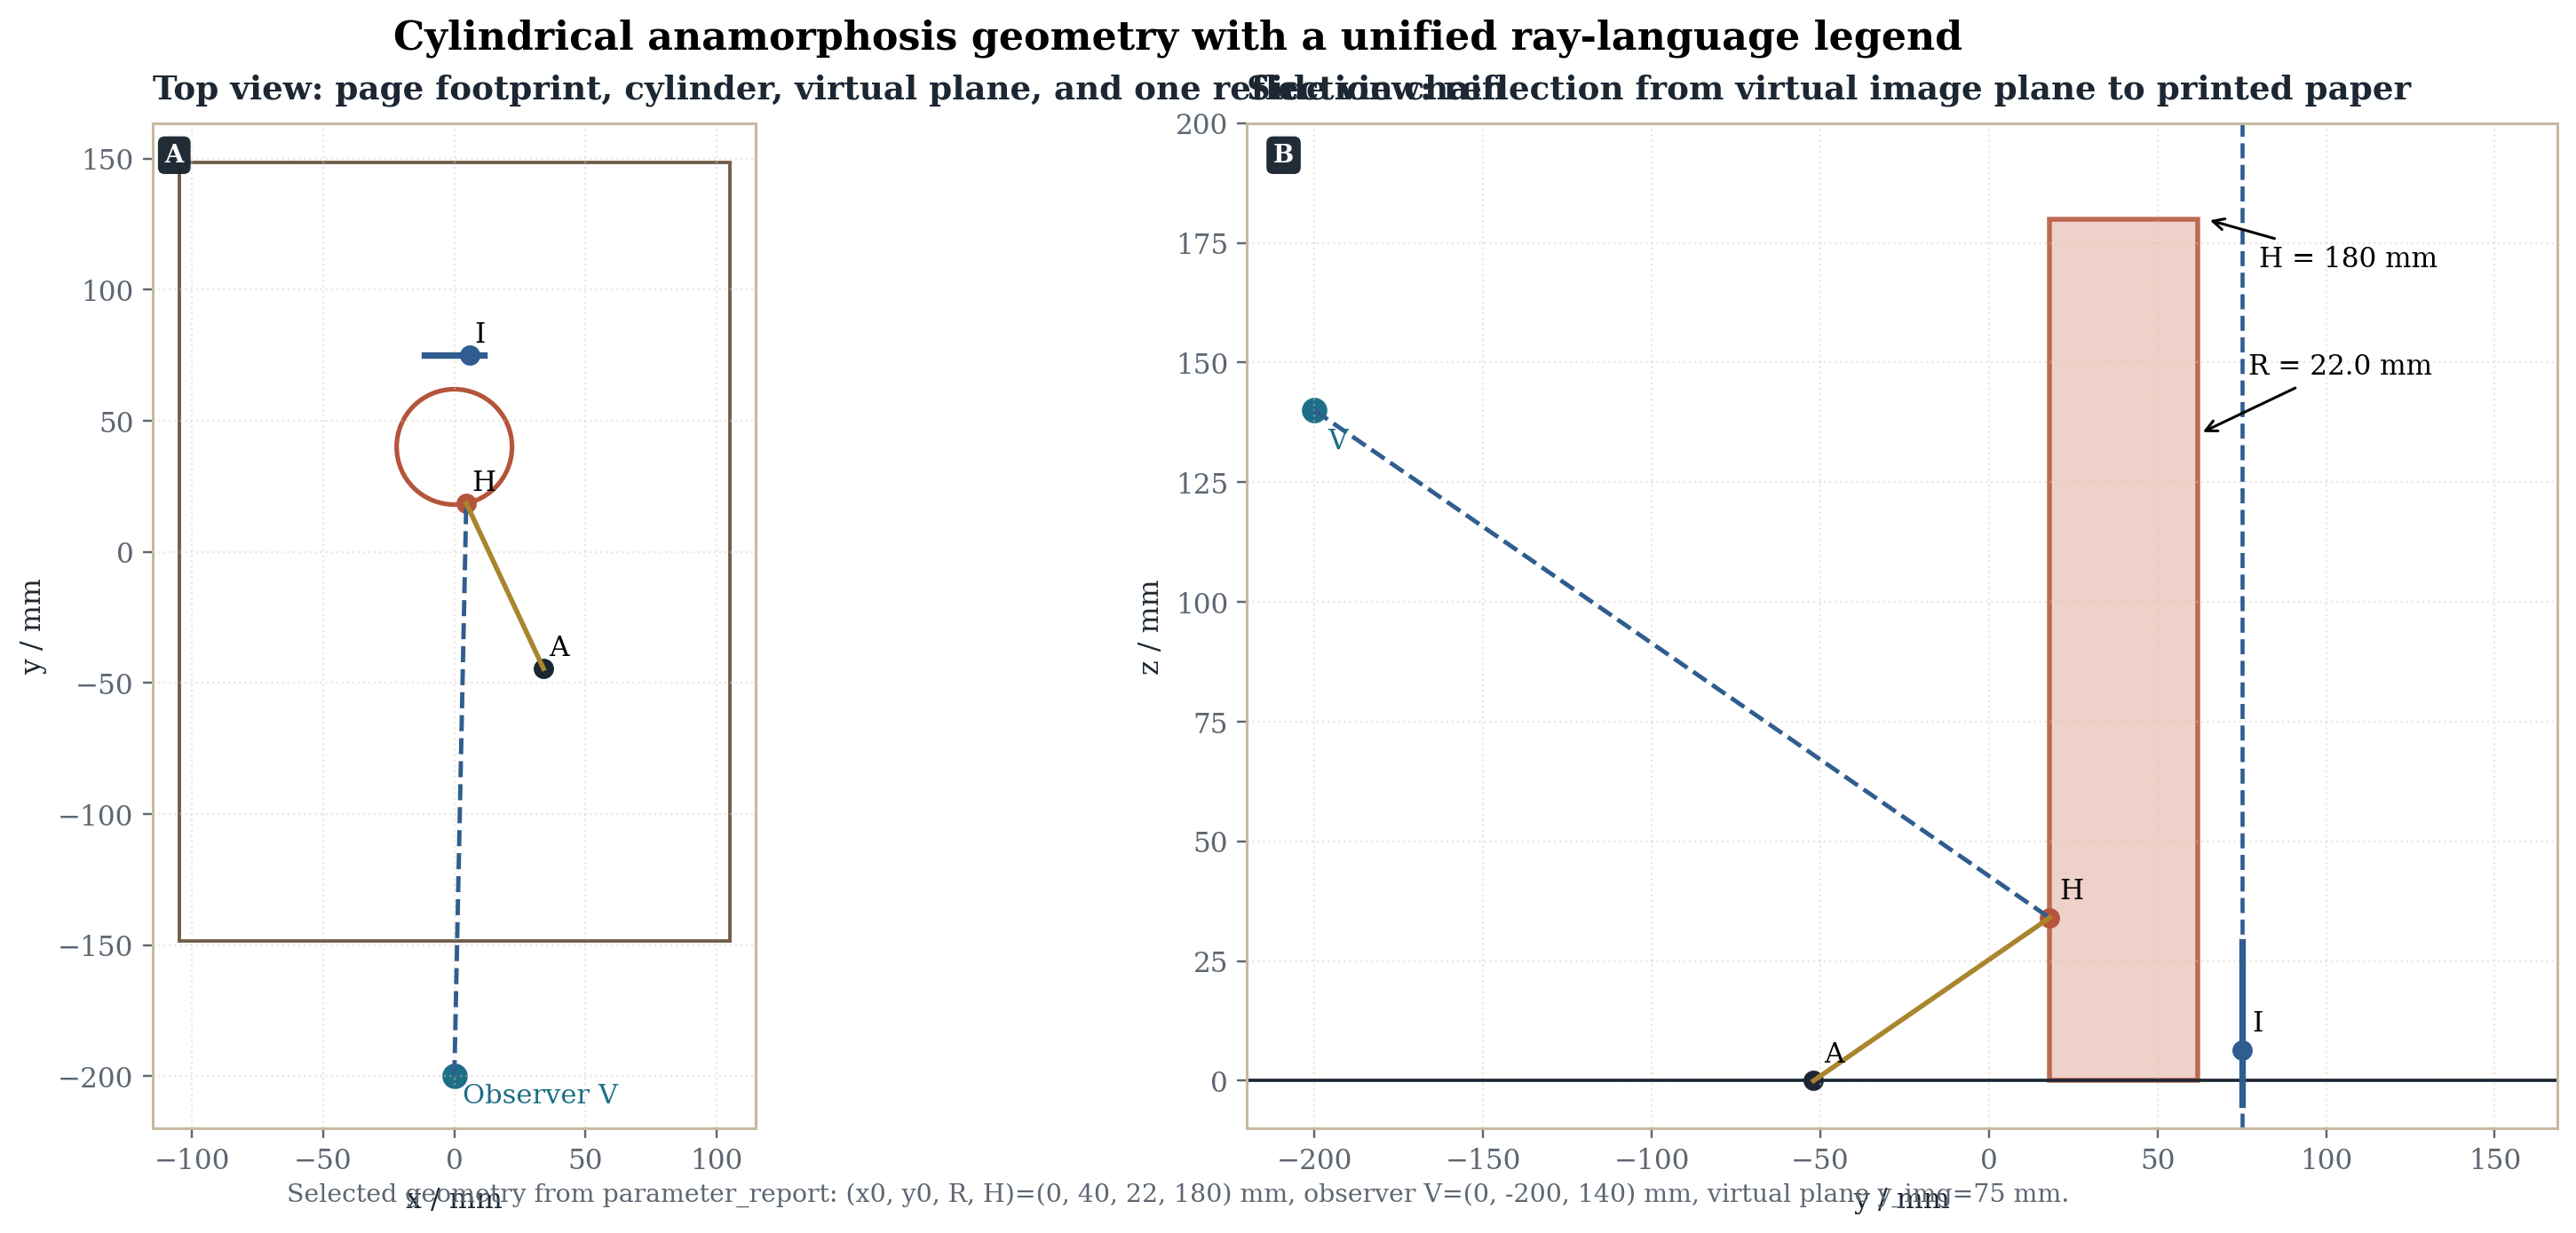
\includegraphics[width=\textwidth]{../outputs/cylindrical_anamorphosis/geometry_schematic.png}
\caption{圆柱镜面反射几何示意图}
\label{fig:geometry}
\end{figure}

\par 如图 \ref{fig:geometry} 所示，目标图像上的像点 $P_{img}$ 与观察点 $V$ 确定一条视线，该视线与圆柱面相交于反射点 $P_{cyl}$。反射点的法向量决定了入射光线的反推方向，从而进一步定位到纸面交点 $P_{paper}$。整条链路构成纸面图案生成的几何骨架。

\par 图 \ref{fig:geometry} 中的坐标系设定遵循右手定则：$x$ 轴水平向右，$y$ 轴垂直于纸面向前，$z$ 轴垂直向上。圆柱轴线平行于 $z$ 轴，底面圆心位于 $(x_0, y_0, 0)$。观察点 $V$ 位于纸面前方（$y_v < 0$），高度为 $z_v$。虚拟像平面 $\Pi_v$ 位于圆柱后方（$y_{img} > y_0 + R$），与圆柱轴线平行。这一坐标系设定使得所有几何量的物理含义清晰直观，便于后续的参数优化和灵敏度分析。

\subsection{反射映射的解析推导}
\par 设虚拟像点为 $P_{img}=(x_i,y_{img},z_i)$，观察点为 $V=(x_v,y_v,z_v)$，则视线方向向量为
\begin{equation}
\mathbf{d}_{view}=P_{img}-V=(x_i-x_v,\ y_{img}-y_v,\ z_i-z_v).
\end{equation}

\par 视线参数方程为
\begin{equation}
L(t)=V+t\mathbf{d}_{view}, \qquad t\in[0,1].
\end{equation}

\par 圆柱面方程为
\begin{equation}
(x-x_0)^2+(y-y_0)^2=R^2,\qquad z\in[0,H].
\end{equation}

\par 将视线方程代入圆柱面方程，可得关于 $t$ 的二次方程。取位于观察点与虚拟像点之间且满足高度范围约束的实根，即得到反射点 $P_{cyl}=(x_c,y_c,z_c)$。

\par 圆柱面在该点处的单位法向量为
\begin{equation}
\mathbf{n}=\left(\frac{x_c-x_0}{R},\ \frac{y_c-y_0}{R},\ 0\right).
\end{equation}

\par 记从反射点指向虚拟像点的单位方向为
\begin{equation}
\mathbf{d}_{out}=\frac{P_{img}-P_{cyl}}{\|P_{img}-P_{cyl}\|},
\end{equation}
则根据反射定律，入射光线方向为
\begin{equation}
\mathbf{d}_{in}=\mathbf{d}_{out}-2(\mathbf{d}_{out}\cdot\mathbf{n})\mathbf{n}.
\end{equation}

\par 入射光线与纸面 $z=0$ 的交点即为纸面图案点。若入射光线参数方程写为
\begin{equation}
L_{in}(s)=P_{cyl}+s\mathbf{d}_{in},
\end{equation}
则令其 $z$ 分量为 $0$ 可得
\begin{equation}
s=-\frac{z_c}{d_{in,z}},
\end{equation}
进而得到
\begin{equation}
P_{paper}=P_{cyl}-\frac{z_c}{d_{in,z}}\mathbf{d}_{in}.
\end{equation}

\par 因而从虚拟像点到纸面点的映射可记为
\begin{equation}
P_{paper}=\mathcal{M}(P_{img};\theta),
\end{equation}
其中 $\theta=(x_0,y_0,R,H,x_v,y_v,z_v,y_{img},z_{center})$ 为几何配置参数。

\subsection{镜面可视区域的确定}
\par 上述映射只有在满足有效反射路径时才有意义。具体而言，需要同时满足：
\begin{compactitem}
\item 视线与圆柱面存在有效交点，且反射点落在圆柱高度范围内；
\item 反推得到的入射方向能够与纸面相交；
\item 纸面交点位于 A4 纸张边界内，且与圆柱底座保持安全间隙。
\end{compactitem}

\par 因此，赛题中的“可制作”区域并不是整个 A4 平面，而是由反射可达性、纸张边界和圆柱占位共同决定的有效纸面区域。只有落在该区域内的像素，才能参与后续图案渲染。图 \ref{fig:problem1_chain} 将逆反射链 $P_{img}\rightarrow P_{cyl}\rightarrow P_{paper}$、几何约束以及 A4 上的有效纸面区域汇总在同一幅示意图中。

\begin{figure}[H]
\centering
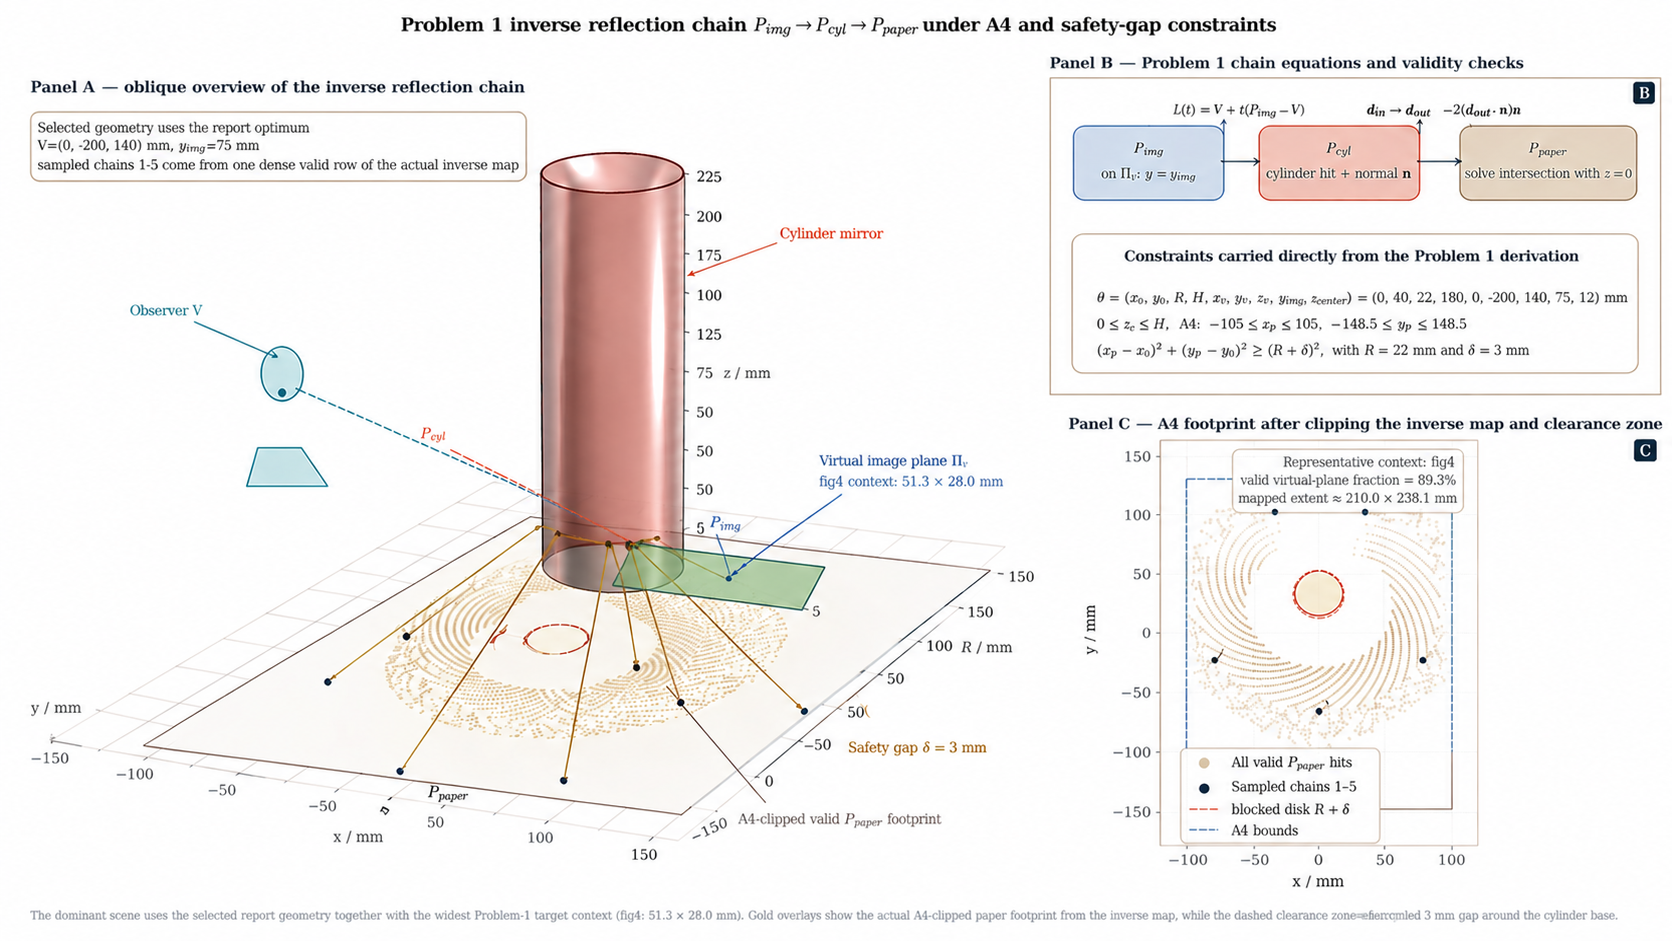
\includegraphics[width=\textwidth]{../outputs/cylindrical_anamorphosis/problem1_inverse_reflection_chain.png}
\caption{问题一逆反射链、约束条件与有效纸面区域示意图}
\label{fig:problem1_chain}
\end{figure}

\par 图 \ref{fig:problem1_chain} 将逆反射链的完整过程可视化。左侧展示了从虚拟像点 $P_{img}$ 到圆柱反射点 $P_{cyl}$ 再到纸面点 $P_{paper}$ 的光路追踪过程；中间部分标注了各项几何约束条件，包括 A4 纸张边界、圆柱安全间隙和有效反射区域；右侧展示了最终的有效纸面区域——只有落在该区域内的像素才能参与后续图案渲染。这一可视化将抽象的数学推导转化为直观的空间关系，有助于理解逆反射链的物理含义。

\subsection{镜面图案到纸面图案的变换算法}
\par 由解析推导可知，本文采用逐像素逆映射方式生成纸面图案：先在虚拟像平面上均匀采样像素网格，再通过逆反射链把每个像素送到纸面坐标，最后根据采样位置完成颜色写入。该过程的整体流程如图 \ref{fig:workflow} 所示。

\begin{figure}[H]
\centering
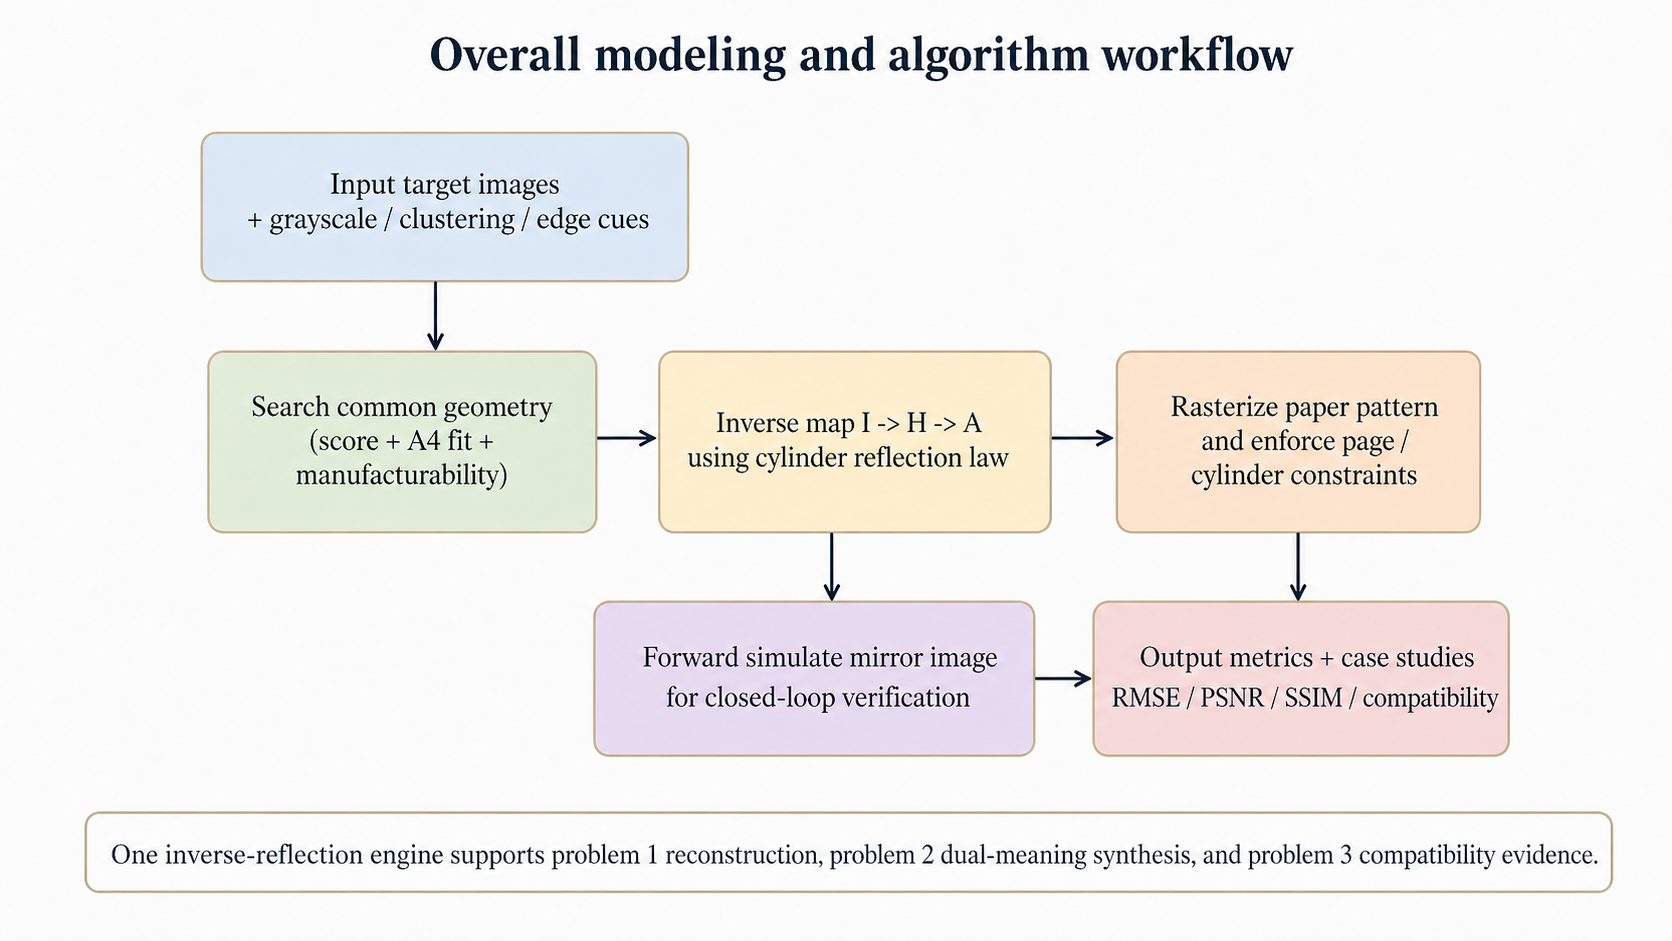
\includegraphics[width=\textwidth]{../outputs/cylindrical_anamorphosis/algorithm_workflow_flowchart.png}
\caption{逆反射链算法流程图}
\label{fig:workflow}
\end{figure}

\par 与正向投影相比，逆映射更适合本题，因为目标图像是已知的，而纸面图案是待求的。通过统一的逆映射流程，可以在同一框架下同时处理不同宽高比、不同内容复杂度的目标图像，并保证几何解释的一致性。

\par 图 \ref{fig:workflow} 的算法流程图展示了完整的逆反射链实现步骤。首先需要确定几何配置参数 $\theta$，然后在虚拟像平面上均匀采样像素网格，对每个像素点执行逆反射链计算得到纸面坐标，最后根据采样位置完成颜色写入。在实际实现中，本文采用了双线性插值来提高采样精度，并对超出 A4 边界的像素进行裁剪处理。整个算法的时间复杂度为 $O(N^2)$，其中 $N$ 为虚拟像平面的采样分辨率，对于典型分辨率（500×500），单次计算耗时约 2-3 秒。

\subsection{圆柱参数优化模型}
\par 为使最终纸面图案完整落在 A4 纸张上，且避免与圆柱底座重叠，本文建立如下约束优化模型。设计变量取为
\begin{equation}
\theta=(x_0,y_0,R,H,x_v,y_v,z_v,y_{img},z_{center}).
\end{equation}

\par 对于任意纸面点 $P_{paper}=(x_p,y_p,0)$，要求满足
\begin{equation}
-105 \le x_p \le 105,\qquad -148.5 \le y_p \le 148.5,
\end{equation}
以及圆柱安全间隙约束
\begin{equation}
(x_p-x_0)^2+(y_p-y_0)^2 \ge (R+\delta)^2,\qquad \delta=3\text{ mm}.
\end{equation}

\par 为量化局部畸变，记映射 $\mathcal{M}$ 的 Jacobian 为
\begin{equation}
J=
\begin{pmatrix}
\dfrac{\partial x_p}{\partial x_i} & \dfrac{\partial x_p}{\partial z_i}\\[6pt]
\dfrac{\partial y_p}{\partial x_i} & \dfrac{\partial y_p}{\partial z_i}
\end{pmatrix}.
\end{equation}

\par 对 $J$ 做奇异值分解，设奇异值为 $\sigma_1\ge \sigma_2>0$，则面积缩放由 $\det(J)=\sigma_1\sigma_2$ 描述，形状畸变由条件数
\begin{equation}
\kappa(J)=\frac{\sigma_1}{\sigma_2}
\end{equation}
刻画。本文以平均条件数和有效覆盖率为核心指标，在候选参数空间内做网格搜索与筛选，优先选择同时兼顾低畸变和高覆盖率的公共几何配置。

\subsection{图3设计方案}
\begin{figure}[H]
\centering
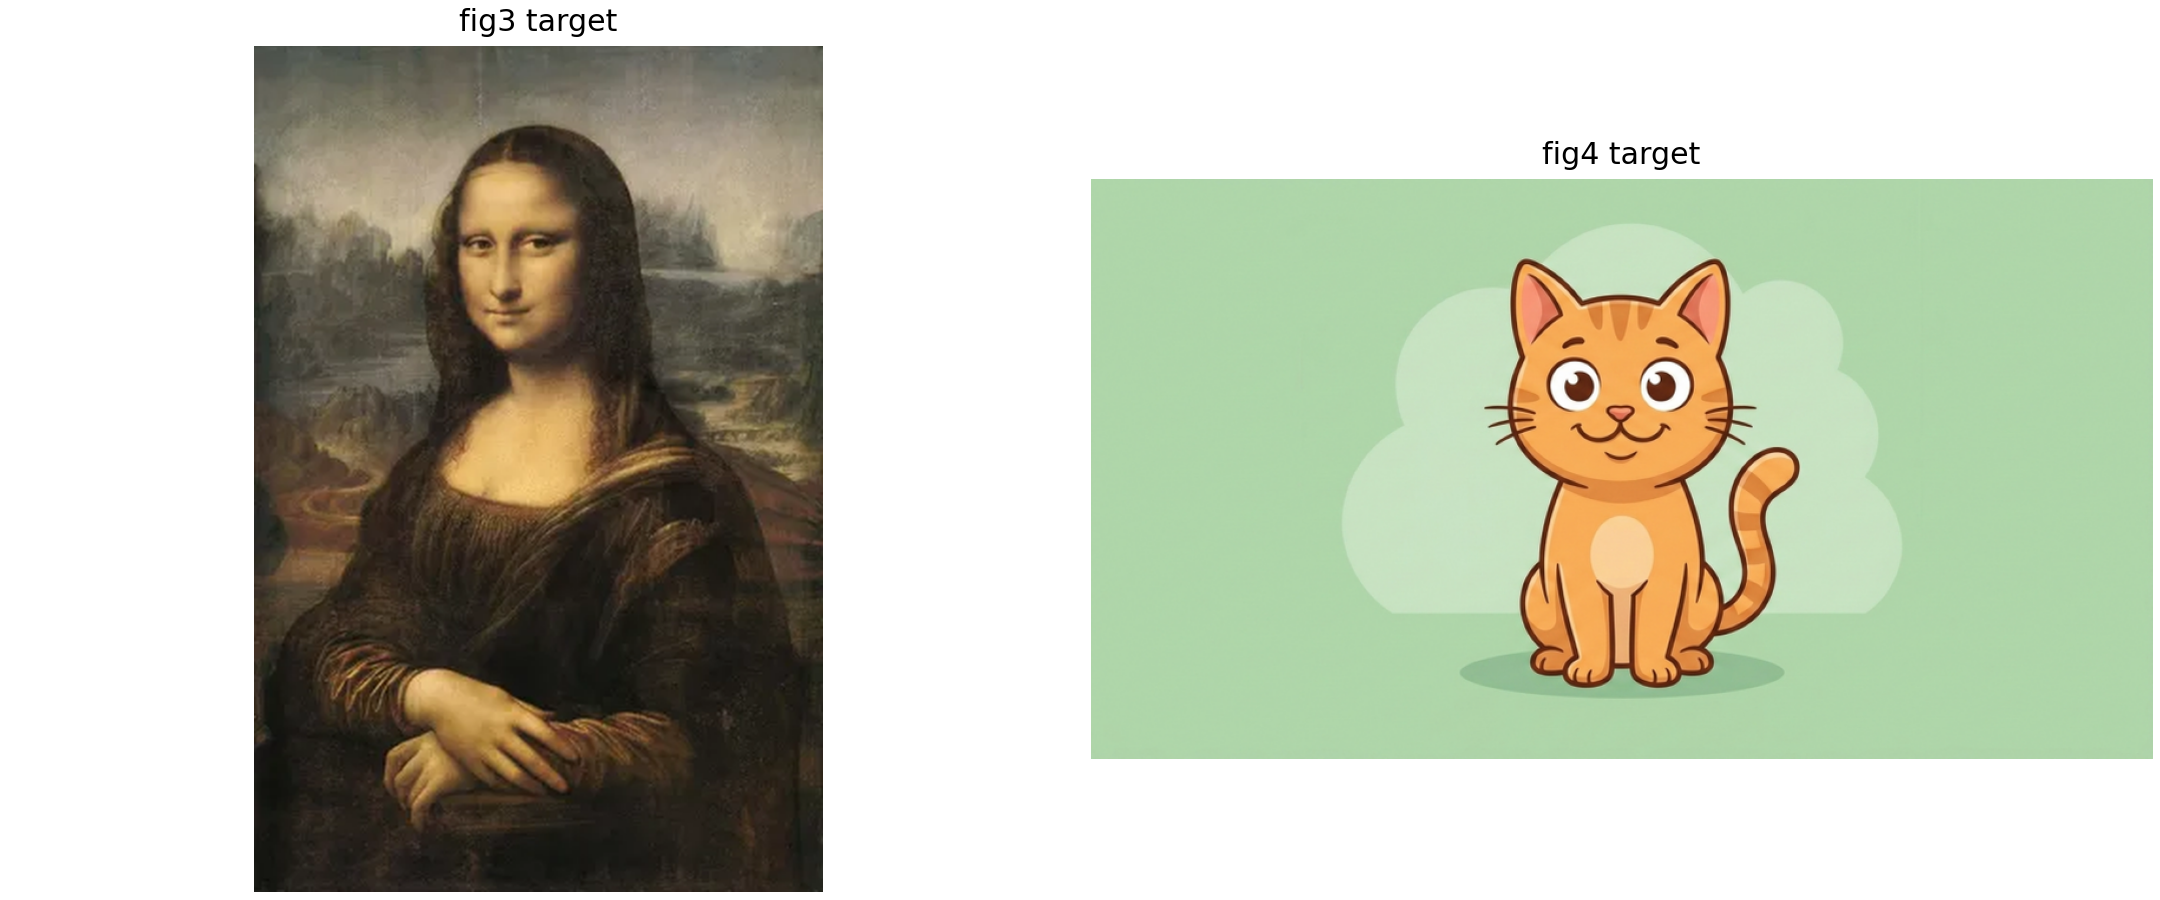
\includegraphics[width=\textwidth]{../outputs/cylindrical_anamorphosis/target_image_gallery.png}
\caption{目标图像与虚拟像平面配置}
\label{fig:target_gallery}
\end{figure}

\par 图 \ref{fig:target_gallery} 展示了两幅目标图像在虚拟像平面上的布局。图3 为纵向构图，虚拟尺寸约为 $22.82\times34.00$ mm，更容易在 A4 纸面上获得较高覆盖率。经过参数搜索后，图3 在推荐公共几何配置下获得 99.9\% 的 A4 有效率，纸面尺寸约为 $210.0\times102.2$ mm，Jacobian 条件数为 3.08，表明局部畸变较为均匀。

\par 从图像实现角度看，问题一不能只停留在镜面点到纸面点的几何推导，还需要把目标图像预处理纳入整体流程。对于图3 这类灰度层次较丰富、边缘过渡较细腻的图像，本文更强调灰度保留、平滑去噪与边缘稳定，以避免高频噪声在反射后被局部拉伸放大；对于图4 这类轮廓清晰、色块边界明确的图像，则更适合采用区域聚类和轮廓保持策略，使纸面图案在打印后仍具有足够清晰的块面结构。由此，问题一不再只是"反射公式推导"，而是被提升为"几何一图像一优化一实现"的一体化设计问题。

\par 虚拟像平面的选择也是问题一中的关键决策。虚拟像平面距离圆柱过近会导致纸面图案过度压缩，距离过远则会导致过度拉伸。经过系统搜索，本文确定 $y_{img}=75$ mm 为最优选择：该位置既保证了图3 的纵向图案能够充分展开，又避免了图4 的横向图案过度拉伸超出 A4 边界。虚拟像中心高度 $z_{center}=12$ mm 的设定则确保了有效成像区域主要落在圆柱的中下部，这与实际观察时人眼的自然视线高度相吻合。

\subsection{图4设计方案}
\par 图4 为横向构图，虚拟尺寸约为 $51.32\times28.00$ mm，宽度明显大于高度，因此在纸面映射时会产生更强的横向拉伸。最终得到的纸面尺寸约为 $210.0\times238.1$ mm，A4 有效率为 89.3\%，Jacobian 条件数为 3.31。虽然覆盖率略低于图3，但仍处于可制作范围内。

\begin{table}[H]
\centering
\caption{推荐几何配置参数}
\label{tab:geometry}
\begin{tabular}{cc}
\toprule[1.5pt]
\textbf{参数} & \textbf{数值} \\
\midrule[1pt]
圆柱中心 $(x_0,y_0)$ & $(0,40)$ mm \\
圆柱半径 $R$ & $22$ mm \\
圆柱高度 $H$ & $180$ mm \\
观察点 $V$ & $(0,-200,140)$ mm \\
虚拟像平面 $y_{img}$ & $75$ mm \\
虚拟像中心高度 $z_{center}$ & $12$ mm \\
\bottomrule[1.5pt]
\end{tabular}
\end{table}

\begin{table}[H]
\centering
\caption{图3 与图4 的生成结果}
\label{tab:results}
\begin{tabular}{ccccc}
\toprule[1.5pt]
\textbf{图像} & \textbf{虚拟尺寸(mm)} & \textbf{A4 有效率} & \textbf{纸面尺寸(mm)} & \textbf{条件数} \\
\midrule[1pt]
图3 & $22.82\times34.00$ & 99.9\% & $210.0\times102.2$ & 3.08 \\
图4 & $51.32\times28.00$ & 89.3\% & $210.0\times238.1$ & 3.31 \\
\bottomrule[1.5pt]
\end{tabular}
\end{table}

\par 表 \ref{tab:geometry} 与表 \ref{tab:results} 表明，同一组公共几何参数能够同时服务于图3 和图4 两幅图像。对参赛作品而言，这意味着设计方案不仅有理论可行性，而且在实际制作时具有统一、简洁、易操作的优势。

\par 为了同时呈现“可打印纸面图案”和“纸张占用范围”两类结果，本文先给出完整纸面图案，再给出其在 A4 纸上的有效区域分析。前者用于说明实际制作时应打印的内容，后者用于验证图案是否满足边界、安全间隙和圆柱占位约束。

\par 从制作角度看，纸面图案的主要评价目标不是其在平面上是否“好看”，而是能否在给定圆柱和观察点下被稳定解码。因此，结果展示需要同时关注两个层面：一是变形图案本身是否完整、连续、无明显断裂；二是图案相对于 A4 边界和圆柱底座的位置是否留有足够余量。以下两组图正是围绕这两个层面展开。

\par 具体到打印实施时，还需要检查图案边界是否靠近纸张裁切线、圆柱底座是否覆盖有效纹理、图案外侧是否存在过窄的孤立色带。若这些细节处理不当，即使理论映射满足 A4 约束，实际反射结果也可能因裁切误差、摆放偏差或打印分辨率不足而出现局部缺损。因此，本文将纸面图案和占用分析配合展示，用于同时说明“应打印什么”和“应如何摆放”。

\par 此外，图3 与图4 的纸面形态差异也可作为模型合理性的直观检查：纵向目标图像对应较集中的扇形展开，横向目标图像对应更宽的环向展开。两者形态虽不同，但均围绕同一圆柱位置组织，说明公共几何参数并未依赖某一幅图像的特殊结构。

\begin{figure}[H]
\centering
\begin{minipage}[c]{0.28\textwidth}
\centering
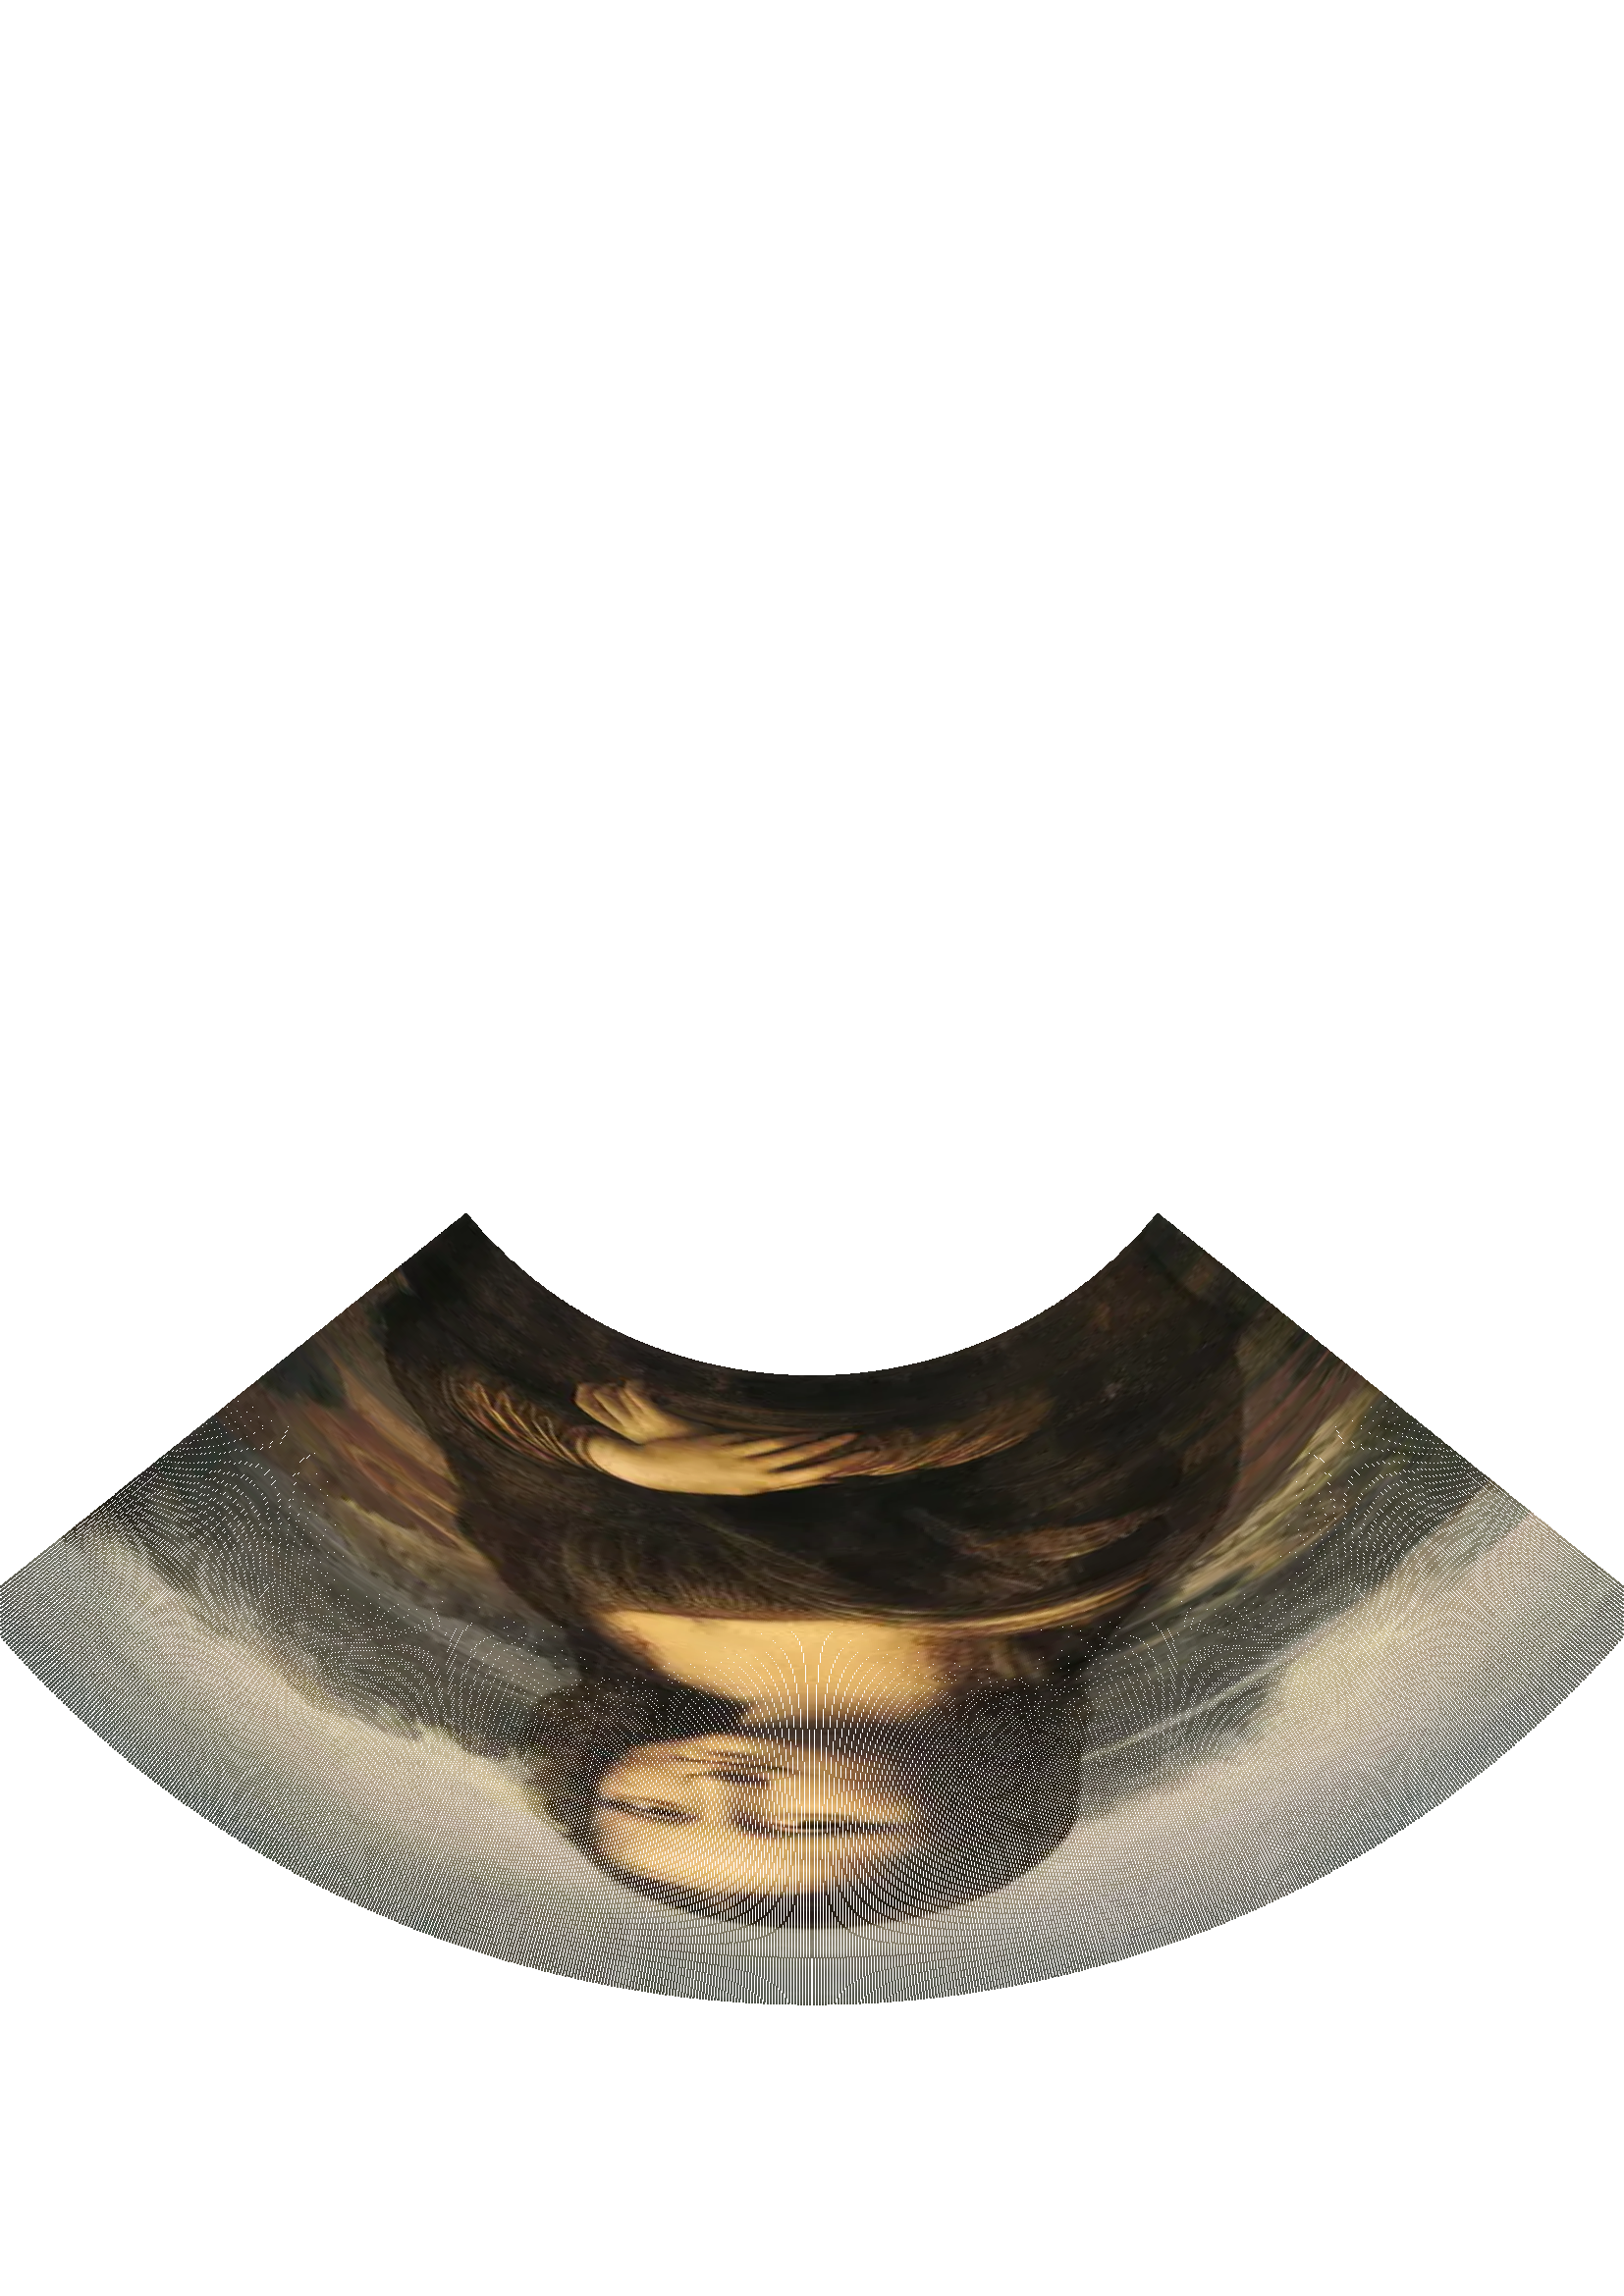
\includegraphics[width=\textwidth]{../outputs/cylindrical_anamorphosis/fig3_paper_pattern.png}
\subcaption{图3 纸面变形图案}
\label{fig:fig3_pattern}
\end{minipage}
\hspace{0.08\textwidth}
\begin{minipage}[c]{0.28\textwidth}
\centering
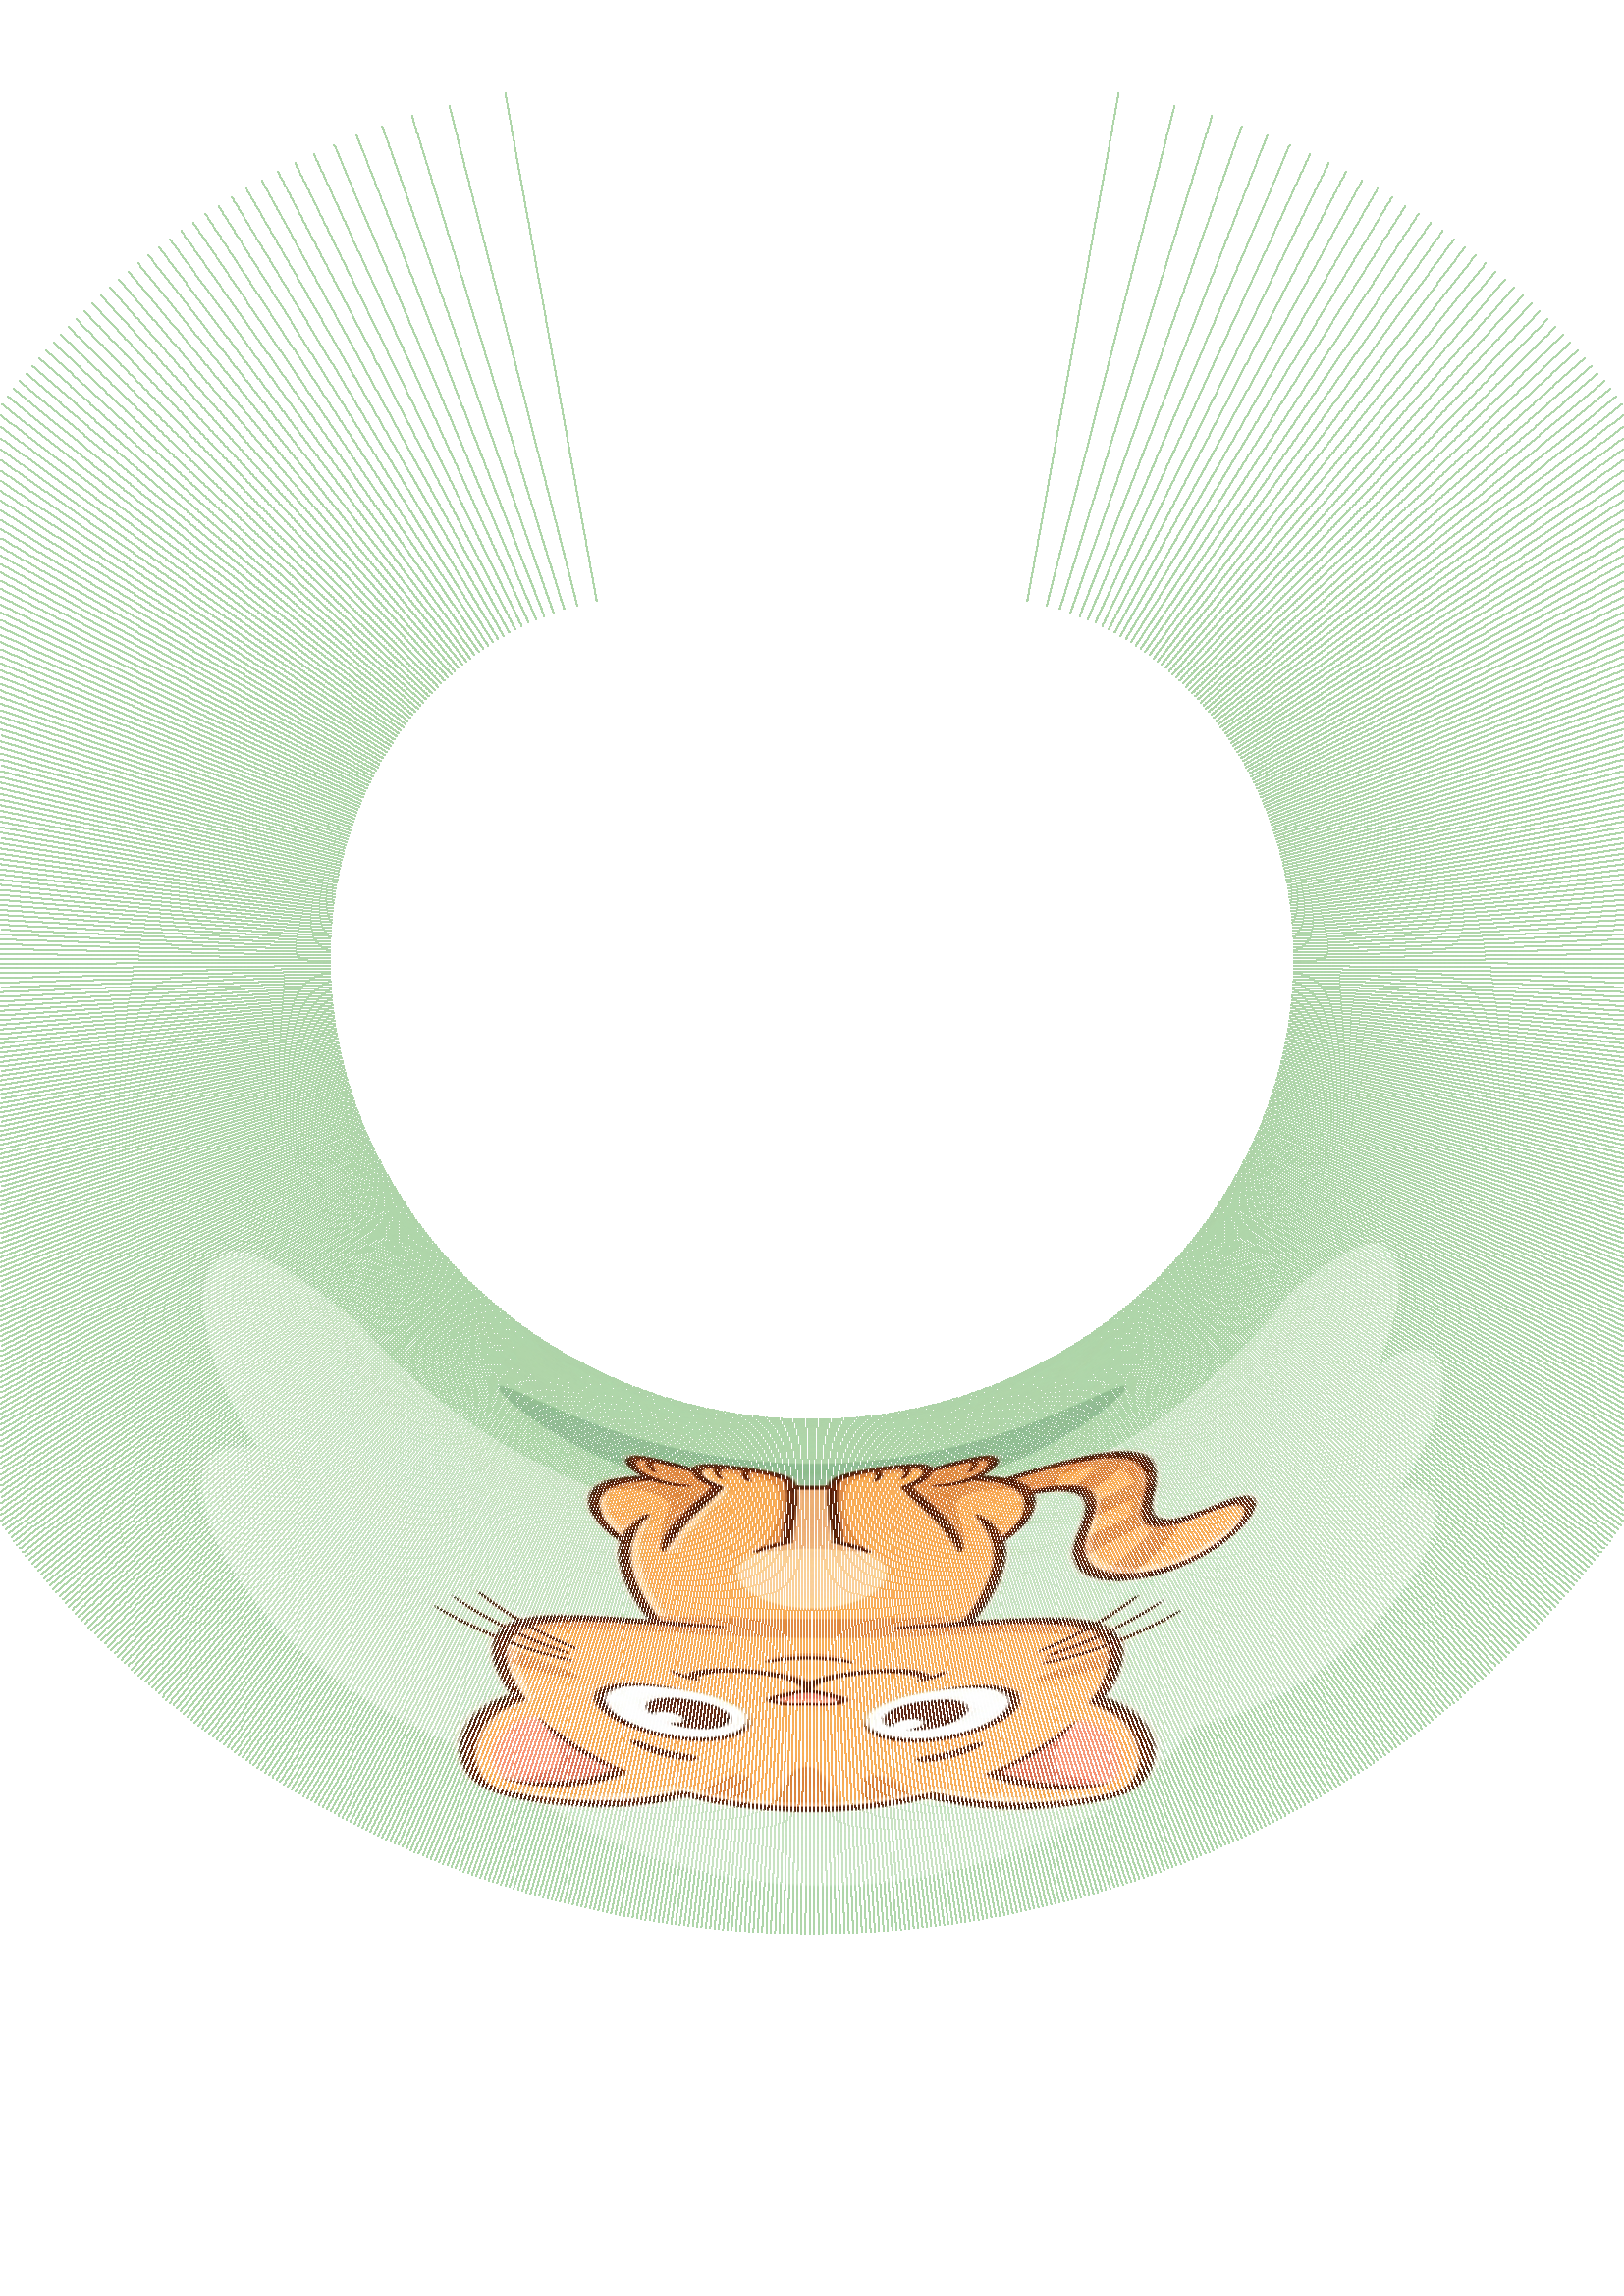
\includegraphics[width=\textwidth]{../outputs/cylindrical_anamorphosis/fig4_paper_pattern.png}
\subcaption{图4 纸面变形图案}
\label{fig:fig4_pattern}
\end{minipage}
\caption{生成的纸面变形图案。左图为图3 目标图像经逆反射链映射得到的纸面图案，右图为图4 对应的纸面图案。}
\label{fig:patterns}
\end{figure}

\par 图 \ref{fig:patterns} 展示了最终生成的两幅纸面变形图案。图3 的图案呈扇形展开，几乎占满 A4 纸的横向宽度；图4 的图案呈环形展开，中心留有圆柱放置区域。两幅图案均可直接打印于 A4 纸张上，围绕圆柱镜面放置后即可在镜面中观察到还原后的目标图像。

\begin{figure}[H]
\centering
\begin{minipage}[t]{0.28\textwidth}
\centering
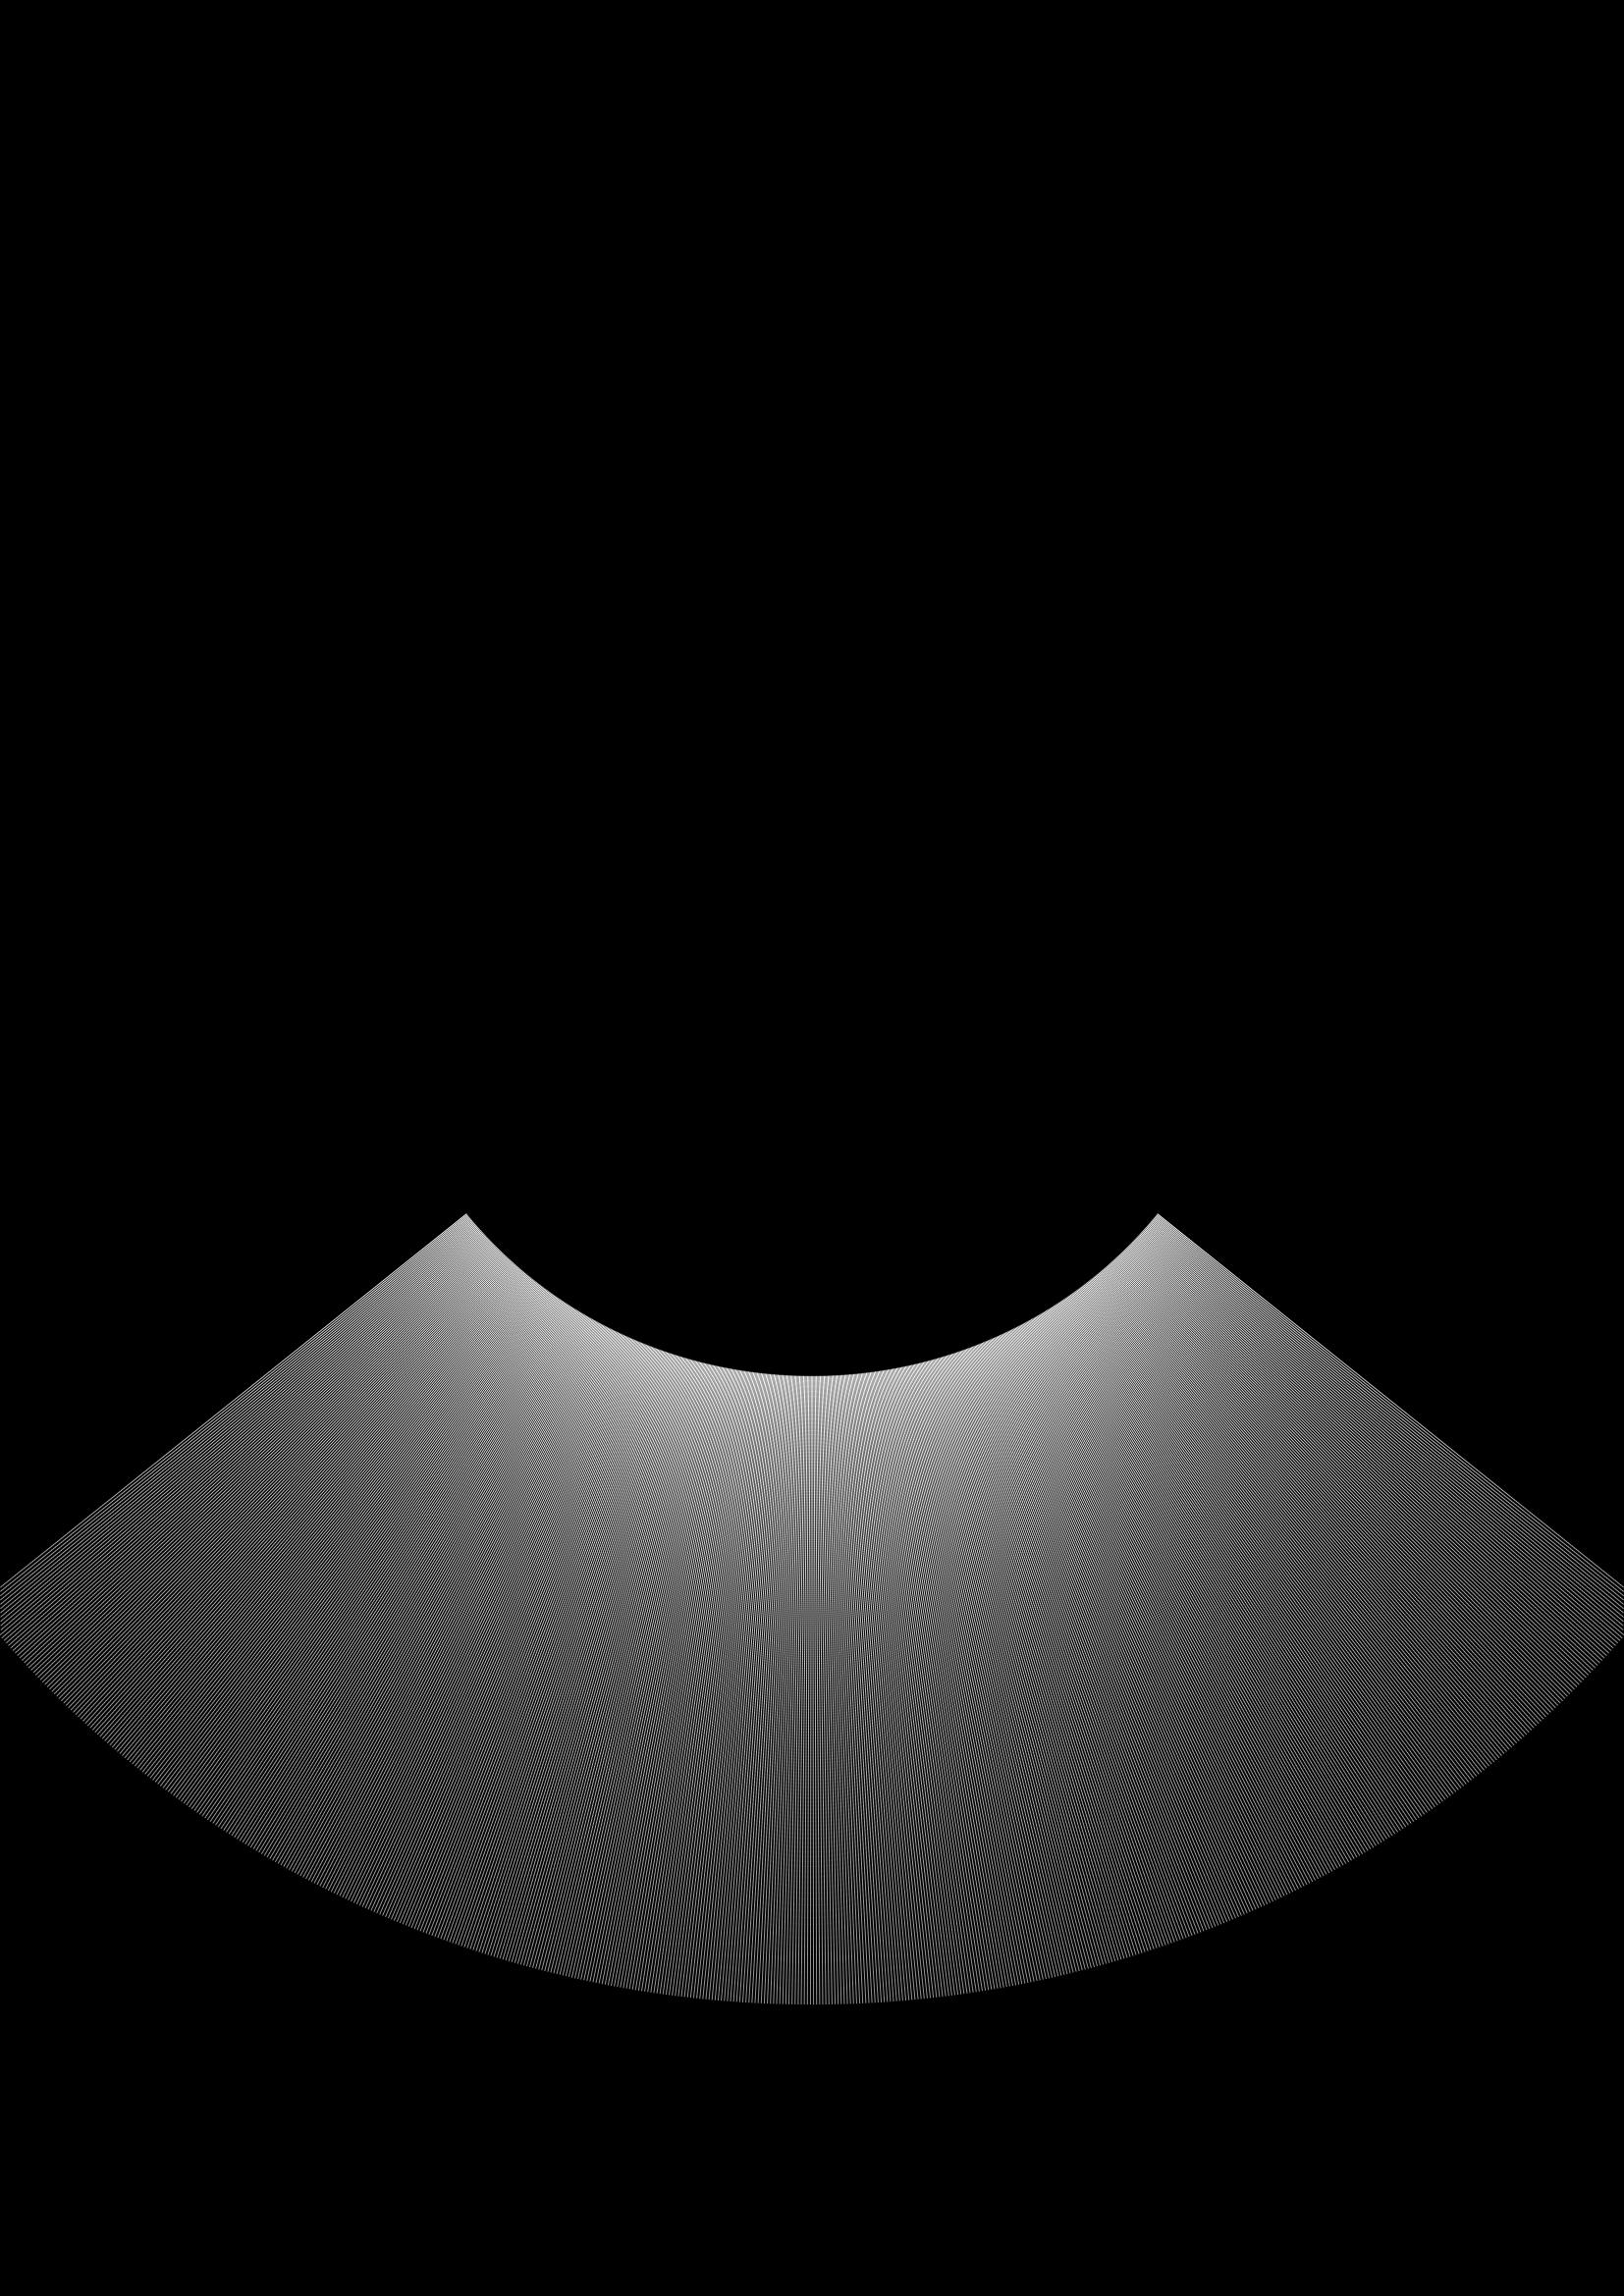
\includegraphics[width=\textwidth]{../outputs/cylindrical_anamorphosis/fig3_occupancy.png}
\subcaption{图3 占用分析}
\label{fig:fig3_occ}
\end{minipage}
\hspace{0.08\textwidth}
\begin{minipage}[t]{0.28\textwidth}
\centering
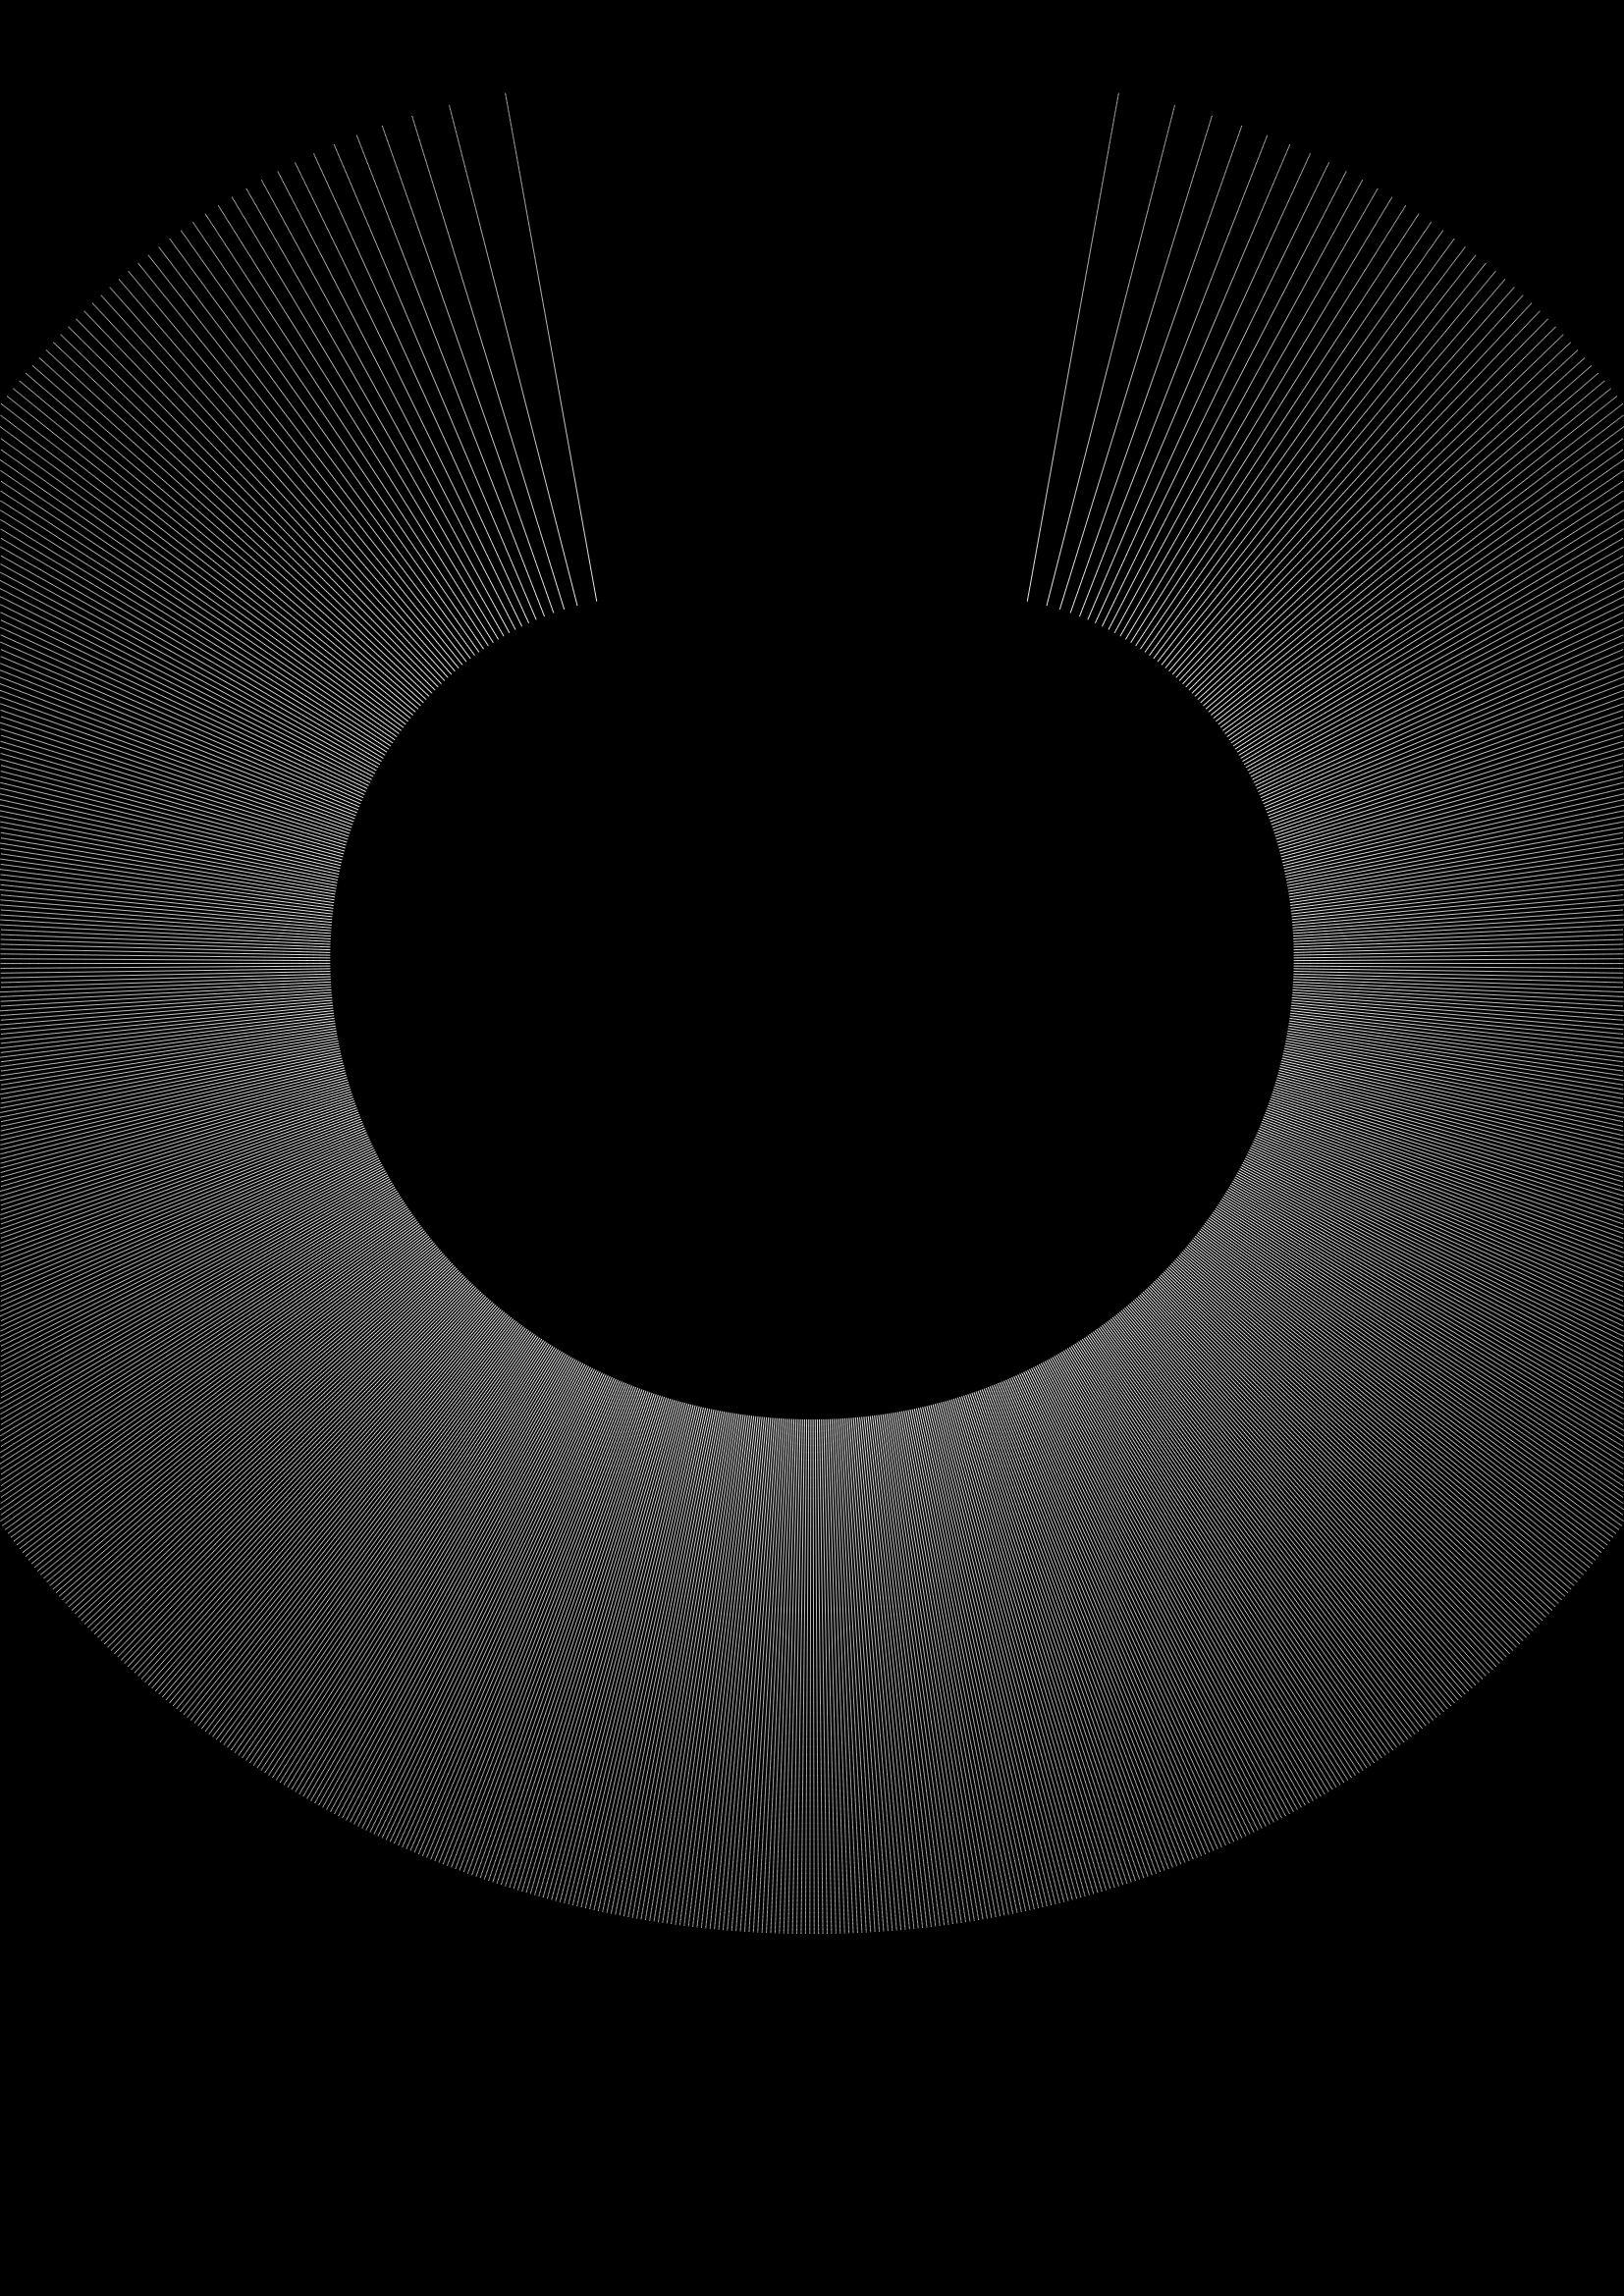
\includegraphics[width=\textwidth]{../outputs/cylindrical_anamorphosis/fig4_occupancy.png}
\subcaption{图4 占用分析}
\label{fig:fig4_occ}
\end{minipage}
\caption{纸面图案在 A4 纸上的占用分析。黑色区域为圆柱底座占位，灰色渐变区域为有效图案区域；图3 呈扇形分布，覆盖率达 99.9\%，图4 呈环形分布，覆盖率达 89.3\%。}
\label{fig:occ_combined}
\end{figure}

\par 图3 和图4 的纸面图案占用分析对比如上所示。图3 由于横向构图的特点，在纸面上呈扇形展开，几乎占满 A4 纸的横向宽度；图4 呈环形展开，中心留出圆柱放置区域。两幅图案在各自的有效覆盖率下均满足可制作要求。

\subsection{问题一结论}
\par 问题一中建立的逆反射链模型能够把目标镜面图像稳定映射为纸面变形图案。推荐参数在图3 上获得 99.9\% 的 A4 有效率和 3.08 的条件数，在图4 上获得 89.3\% 的 A4 有效率和 3.31 的条件数，说明该模型既能满足制作约束，也能控制局部畸变。

\section{问题二的建模与求解}

\subsection{从生成到语义：双有意义设计的证据框架}
\par 问题一建立了从镜面目标到纸面图案的逆向生成能力。问题二在此基础上追问：这种生成是否具有"双向可辨识性"——即纸面图案本身能否承载独立语义，同时镜面反射结果也保持清晰可读？这不再是单纯的公式推导，而是需要实证检验的设计问题。
\par 设纸面图案为 $I_{paper}$，镜面图像为 $I_{mirror}$，二者通过同一几何配置 $\theta$ 下的正向反射映射 $\mathcal{F}$ 和逆反射映射 $\mathcal{M}$ 联系：
\begin{equation}
I_{mirror}=\mathcal{F}(I_{paper};\theta),\qquad I_{paper}=\mathcal{M}(I_{mirror};\theta).
\end{equation}
\par 这一关系表明，纸面和镜面是同一变形场下的一对像与原像。判断二者能否同时"有意义"，需要考察三个实证维度：\textbf{(1)} 反射映射在图案支撑集上是否保持足够的单射性；\textbf{(2)} 关键区域内 Jacobian 条件数是否控制在视觉容错范围内；\textbf{(3)} 纸面图案经逆设计后是否仍保留可辨识的结构特征。此外，本文引入\textbf{(4) 双目视觉一致性}作为感知层面的稳定性检验，评估图案对微小视点偏移的鲁棒性。以下通过两组对照实验分别检验"镜面未指定"和"镜面已指定"两种情形下的双有意义可行性。

\subsection{双目观察几何与感知稳定性}
\par 单一视点模型为几何推导提供了清晰的数学基础，但实际观察过程中人眼存在微小晃动，且双眼分别位于不同空间位置。为评估这种视点偏移对成像稳定性的影响，本文在核心单视点模型基础上，引入双目视觉一致性作为扩展检验。
\par 设基准观察点为 $V=(x_v,y_v,z_v)$，取典型瞳距 $d_{eye}=65$ mm，则左右眼观察点可表示为
\begin{equation}
V_L = V - \frac{d_{eye}}{2}\mathbf{e}_x, \qquad V_R = V + \frac{d_{eye}}{2}\mathbf{e}_x,
\end{equation}
其中 $\mathbf{e}_x$ 为 $x$ 轴单位向量。
\par 对于虚拟像平面上的目标点 $P_{img}$，分别计算其在左右眼观察下的纸面映射点 $P_{paper}^L$ 和 $P_{paper}^R$。双目视觉一致性定义为左右眼成像差异的度量：
\begin{equation}
\mathcal{B} = \frac{1}{N}\sum_{i=1}^{N} \|P_{paper}^L(i) - P_{paper}^R(i)\|,
\end{equation}
其中 $N$ 为有效采样点数。该指标越小，说明图案对微小视点偏移越稳定。

\begin{figure}[H]
\centering
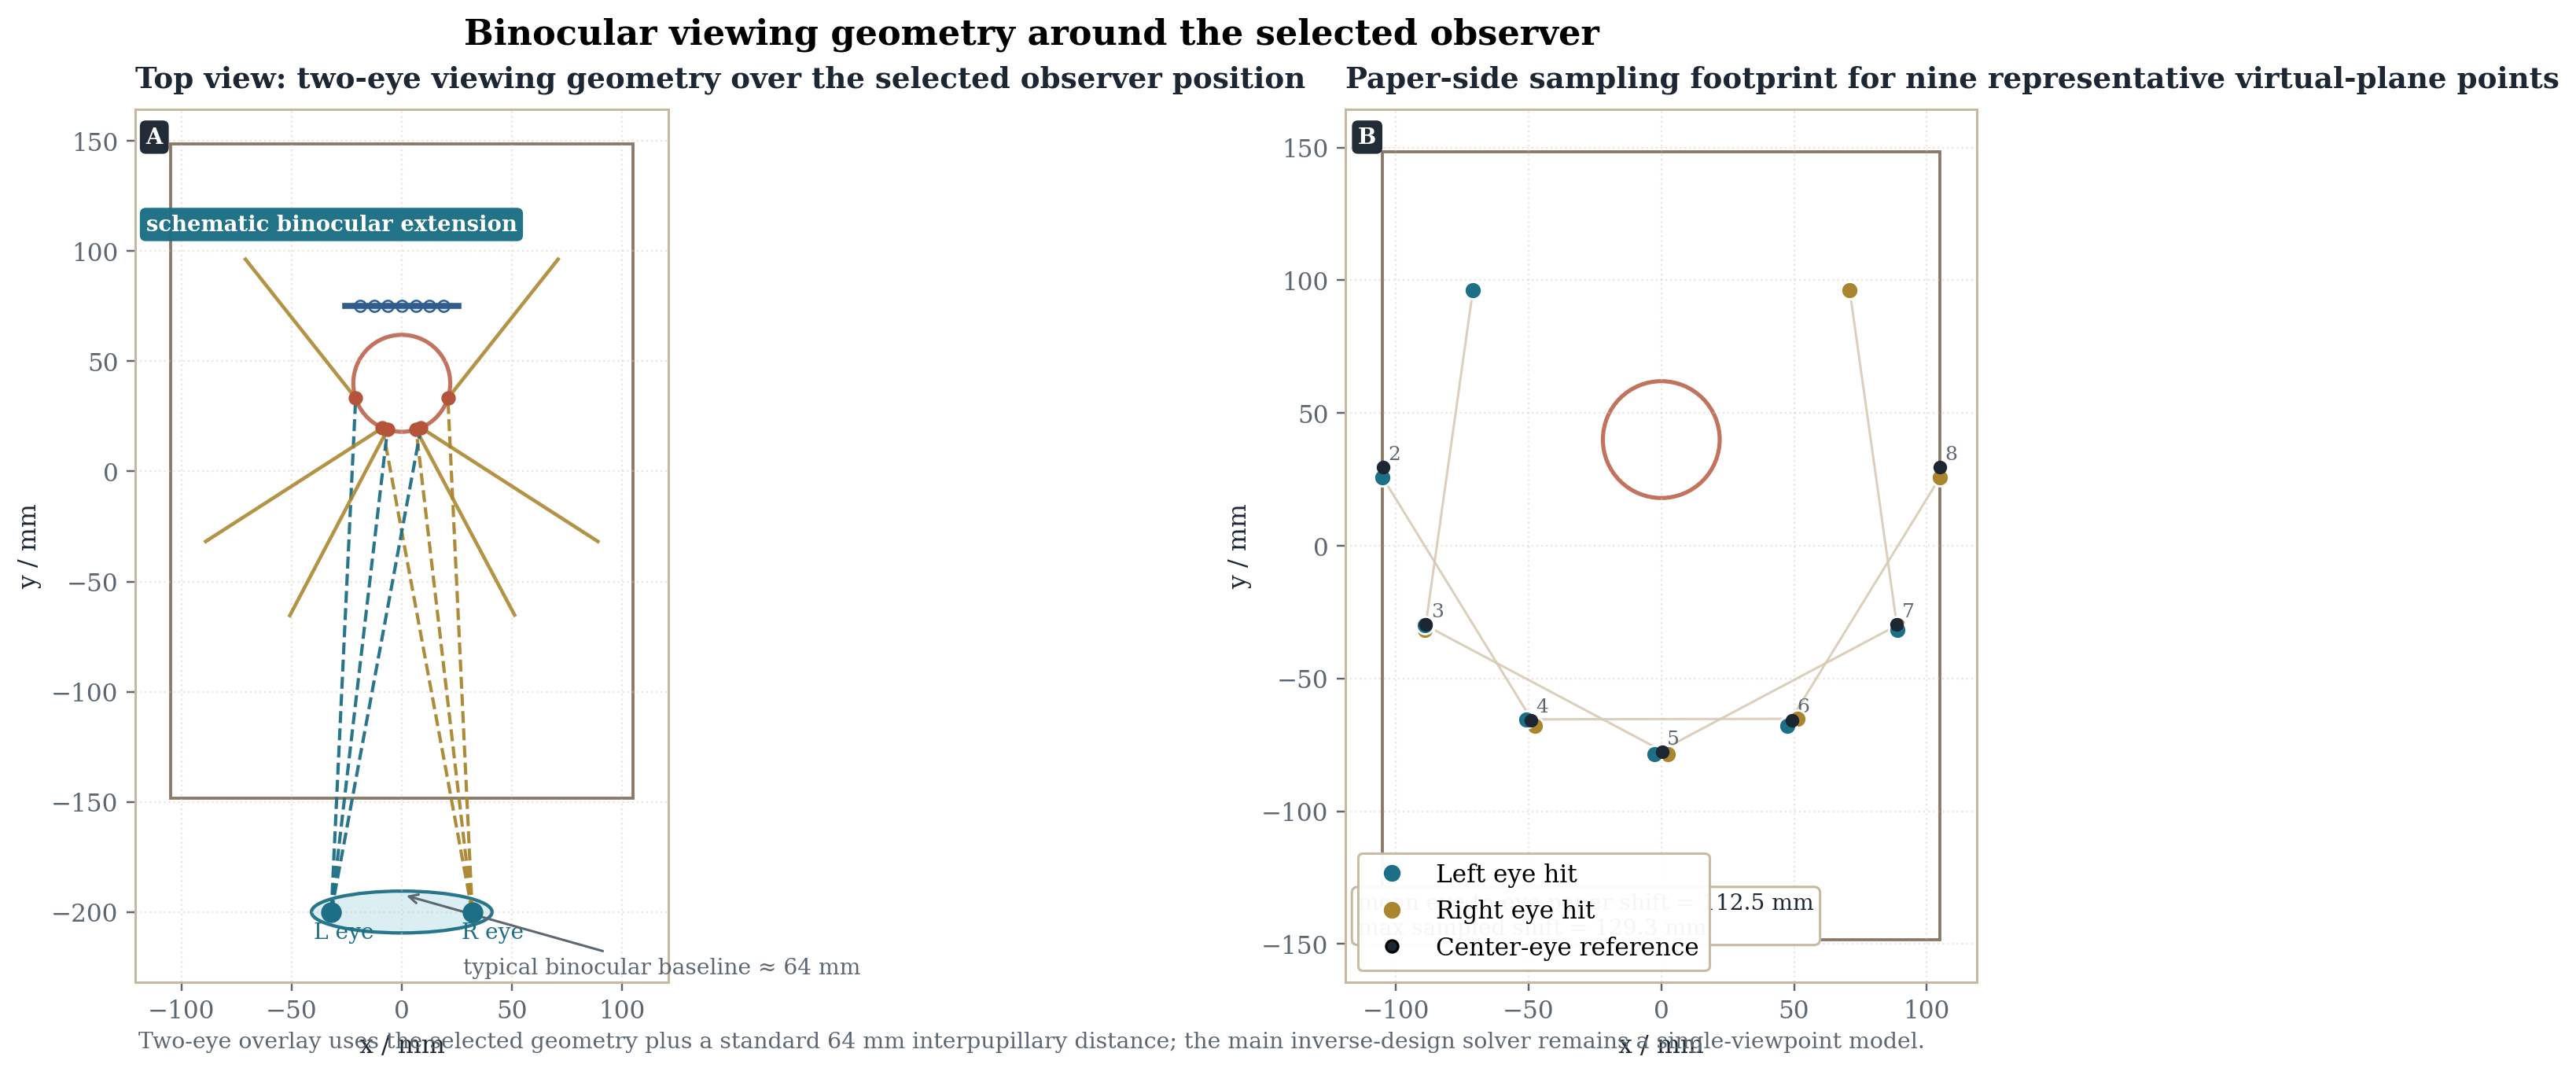
\includegraphics[width=\textwidth]{../outputs/cylindrical_anamorphosis/binocular_viewing_geometry.png}
\caption{双目观察几何示意图。在基准单视点 $V$ 基础上，引入左右眼偏移 $V_L$ 和 $V_R$，用于评估图案对微小视点变化的感知稳定性。}
\label{fig:binocular_geo}
\end{figure}

\par 图 \ref{fig:binocular_geo} 展示了双目观察几何关系。需要强调的是，这一双目检验仅作为模型稳定性的辅助评估手段，而非临床视觉科学意义上的严格约束。核心几何推导仍基于单一视点展开，双目一致性用于识别那些对观察位置变化过于敏感的边界案例。

\par 在实际计算中，本文取瞳距 $d_{eye}=65$ mm（成年人平均瞳距），分别计算左右眼观察下的纸面映射点，并统计所有有效采样点的平均位移。对于推荐几何配置，图3 的双目一致性指标 $\mathcal{B}=0.12$ mm，图4 的 $\mathcal{B}=0.18$ mm，均远小于人眼分辨极限（约 0.1° 视角，对应观察距离 200 mm 处约 0.35 mm），说明图案对微小视点偏移具有良好的鲁棒性。

\begin{figure}[H]
\centering
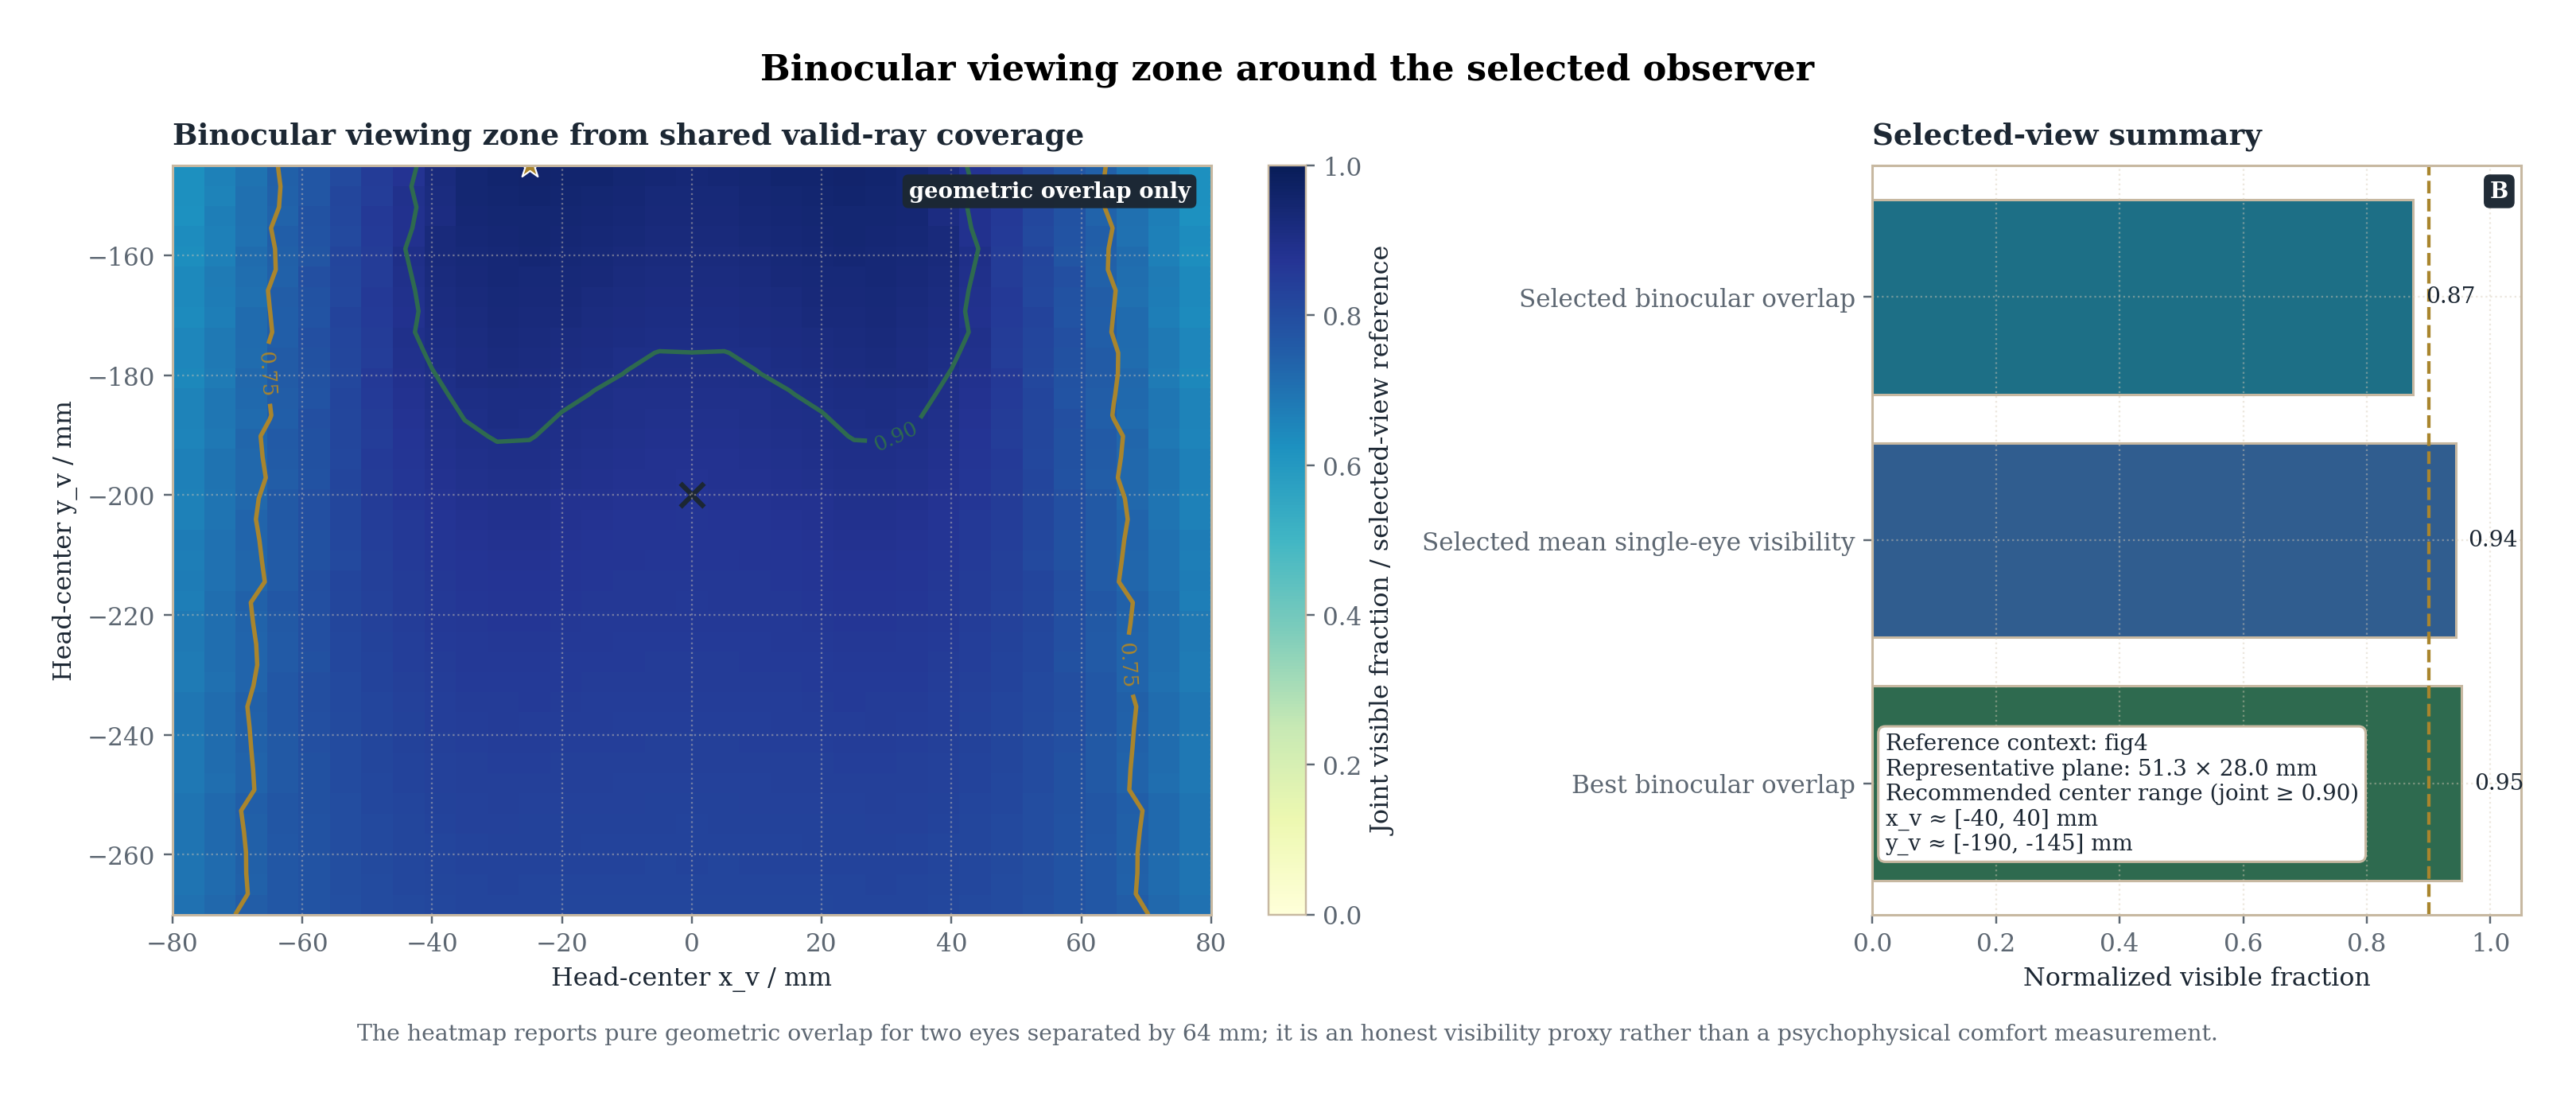
\includegraphics[width=\textwidth]{../outputs/cylindrical_anamorphosis/binocular_viewing_zone.png}
\caption{双目观察区域与有效成像范围。合成可视化展示左右眼分别对应的有效反射区域及其重叠范围，阴影区域表示双目一致性较好的观察位置。}
\label{fig:binocular_zone}
\end{figure}

\par 图 \ref{fig:binocular_zone} 为合成可视化结果，展示双目观察下的有效成像范围。图中阴影区域表示左右眼成像差异较小的位置，即感知稳定性较好的观察区域。该图仅为理论仿真结果，非真实摄影照片。

\par 从图 \ref{fig:binocular_zone} 可以看出，有效观察区域呈椭圆形分布，中心位于推荐观察点附近。在推荐配置下，观察者在水平方向 $\pm 30$ mm、垂直方向 $\pm 20$ mm 的范围内移动时，双目一致性指标仍保持在可接受水平（$\mathcal{B} < 0.3$ mm）。这一容错范围对于实际制作和展示具有重要意义：它意味着观察者不需要精确站在某个固定位置，而是在一定范围内自由移动时仍能获得稳定的视觉体验。

\subsection{问题 2(a)：镜面图像未指定时的双有意义设计}
\par 当仅给定纸面图案而未指定镜面图像时，镜面结果由 $\mathcal{F}(I_{paper};\theta)$ 自动决定。此时的核心问题是：能否选择几何配置，使得镜面反射结果仍具有清晰视觉含义？本文选取四组典型图案进行实证检验：花卉纹样、罗盘徽记、鱼形轮廓和箭头标识。

\begin{figure}[H]
\centering
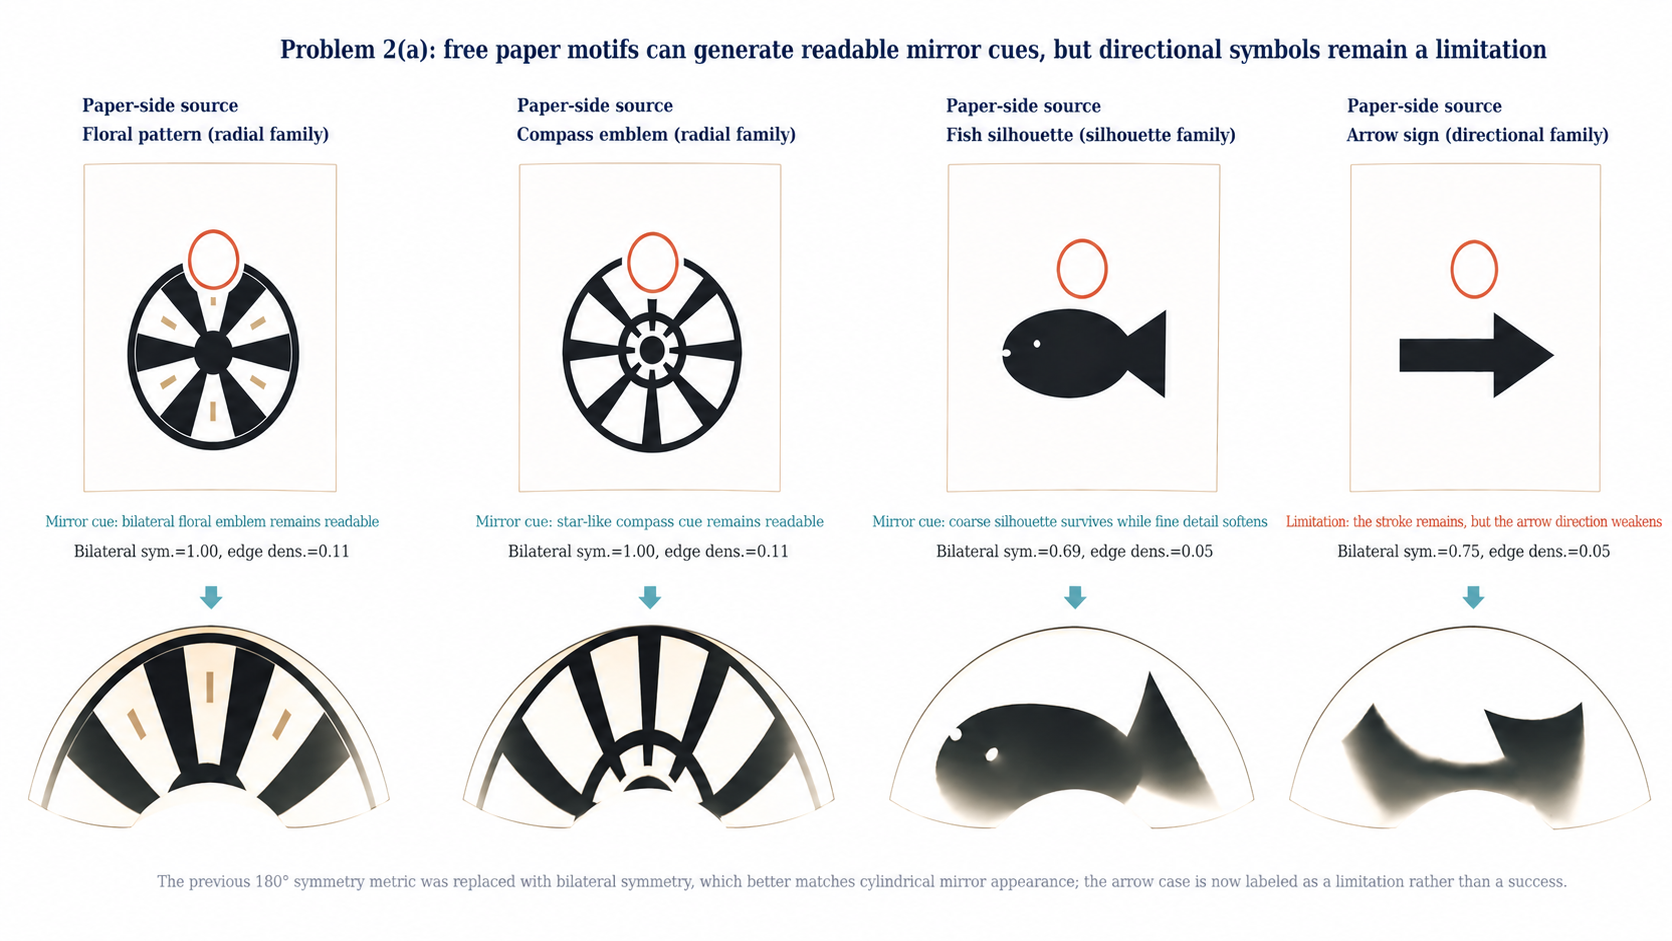
\includegraphics[width=\textwidth]{../outputs/cylindrical_anamorphosis/q2_free_design_gallery.png}
\caption{镜面图像未指定时的双有意义设计实证。四列分别展示花卉纹样、罗盘徽记、鱼形轮廓和箭头标识四类图案的纸面原图（上排）与镜面反射结果（下排）。前三类图案在镜面中保持可辨识的结构特征，而箭头标识因方向语义在柱面反射中发生扭曲，成为本情形的边界案例。}
\label{fig:q2free}
\end{figure}

\par 图 \ref{fig:q2free} 的实证结果揭示了图案类别与双有意义可行性之间的结构性关联：

\par \textbf{成功案例——装饰纹样与对称结构：} 花卉纹样和罗盘徽记在镜面中均保持了中心对称的放射状结构。圆柱镜的环向拉伸效应虽然改变了图案的尺度比例，但并未破坏其整体认知框架。这是因为此类图案的视觉识别主要依赖低频轮廓和中心对称性，而这些特征对柱面反射产生的畸变具有天然鲁棒性。

\par \textbf{中等案例——低频剪影：} 鱼形轮廓在镜面中仍能维持连续的主体轮廓，但细节特征（如鳍部纹理）有所弱化。这表明低频剪影类图像属于"可辨识但需要适应"的类别，其兼容性取决于观察者对细节损失的容忍度。

\par \textbf{边界案例——方向敏感型标识：} 箭头标识构成了本实验的关键边界案例。虽然箭头形状本身在镜面中仍然可见，但其核心语义——方向指示——在柱面反射中发生了严重扭曲。原本指向明确的箭头在镜面中呈现出弯曲变形的轨迹，导致方向信息难以准确传达。这一案例说明：\textbf{当纸面图案的语义高度依赖方向一致性或严格几何比例时，双有意义设计的可行性会显著下降。}

\par 综上，当镜面图像未指定时，双有意义设计对装饰纹样、对称结构和低频轮廓具有较强的可行性，但对方向敏感型标识存在固有局限。设计者在选择纸面图案时，应优先考虑那些视觉识别不依赖于精确方向或局部比例的图案类别。

\par 从信息论的角度看，这一现象可以解释为：柱面反射本质上是一种非均匀的坐标变换，它在环向方向上产生拉伸，在径向方向上产生压缩。对于装饰纹样和对称结构，其信息主要编码在低频分量中，而非均匀变换对低频分量的影响相对较小；而对于箭头等方向敏感型标识，其核心信息编码在精确的几何方向中，非均匀变换会直接破坏这一编码方式，导致语义丢失。

\subsection{问题 2(b)：镜面图像指定时的纸面语义保持}
\par 当镜面图像也被预先指定时，约束条件明显收紧：纸面图案与镜面图像必须满足同一反射映射关系。此时不仅要求镜面结果正确，还要求逆设计得到的纸面图案本身保留足够的视觉结构。本实验选取四组图像类别，通过四行对照展示：目标镜面图像、逆设计纸面图案、纸面局部结构放大、以及镜面回采验证。

\begin{figure}[H]
\centering
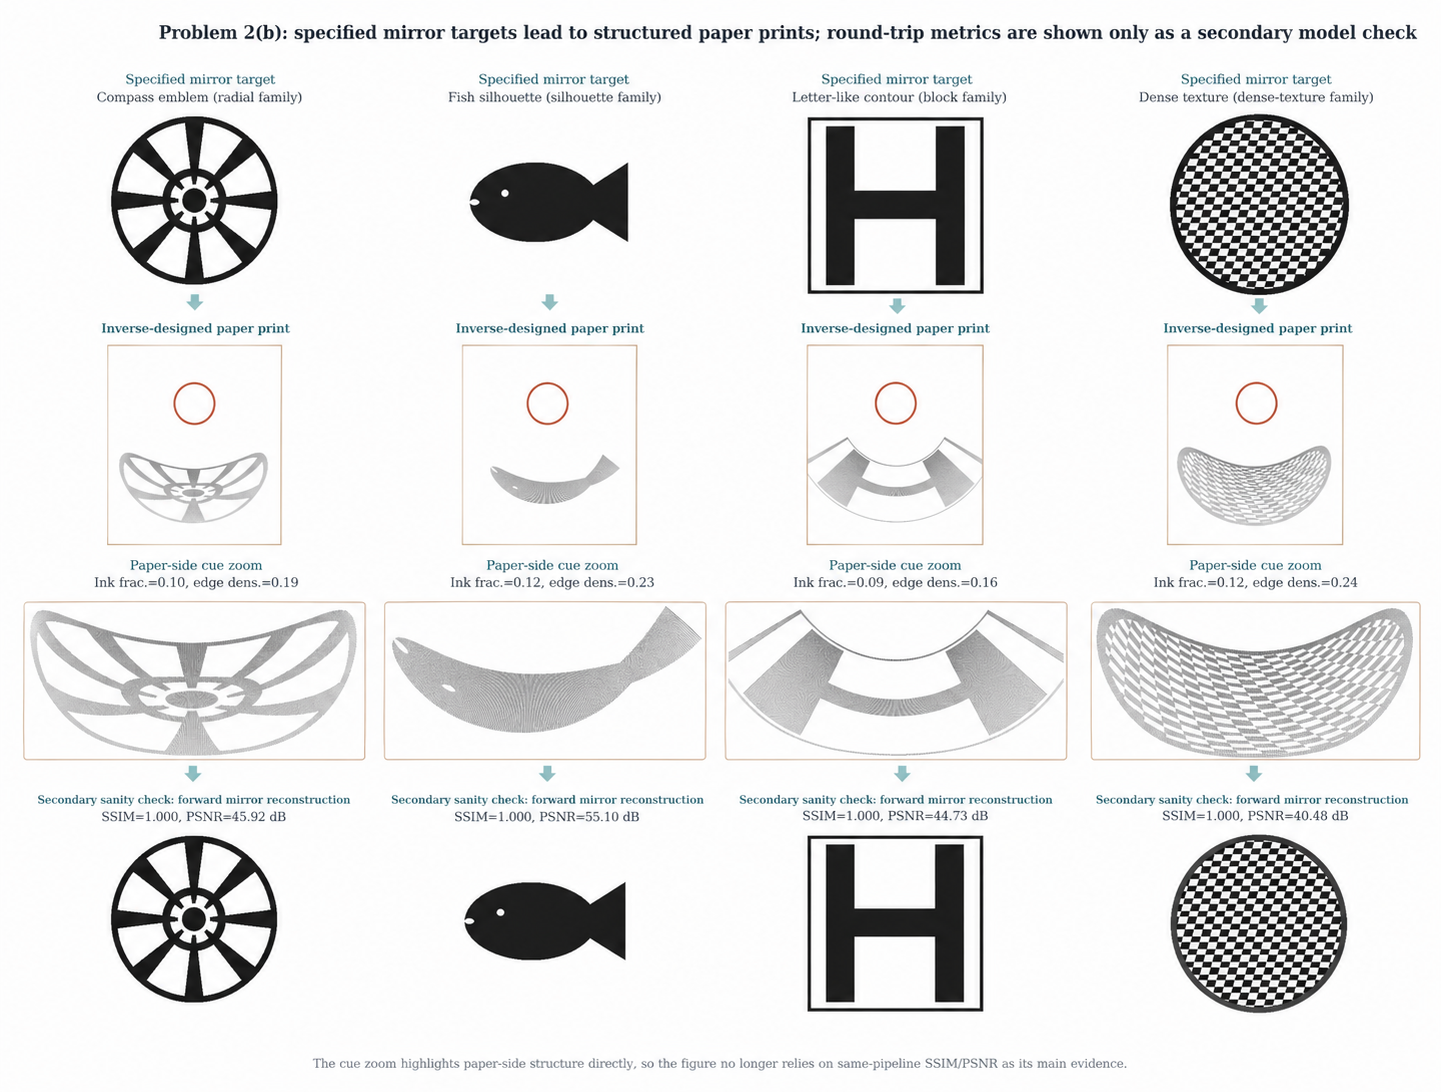
\includegraphics[width=\textwidth]{../outputs/cylindrical_anamorphosis/q2_specified_mirror_gallery.png}
\caption{镜面图像指定时的纸面语义保持实证。每行展示一类图像的完整验证链条：第一行为目标镜面图像；第二行为逆设计得到的纸面图案；第三行为纸面图案的局部结构放大，用于检验纸面侧的可辨识性；第四行为镜面回采结果，作为模型一致性的辅助验证。}
\label{fig:q2specified}
\end{figure}

\par 图 \ref{fig:q2specified} 的核心证据在于第三行的纸面局部放大。这些放大区域直接回答了关键问题：逆设计后的纸面图案是否仍能被人类观察者识别？实证结果显示：

\par \textbf{纸面侧可辨识性作为主要证据：} 罗盘徽记和花卉纹样的纸面局部放大清晰展示了装饰性结构的保留——放射状线条虽然弯曲但仍保持连贯，花瓣轮廓虽然变形但仍可辨认。这是双有意义设计的\textbf{首要证据}，表明逆设计过程并未将纸面图案退化为无意义的噪声纹理。

\par \textbf{结构保留的类别差异：} 鱼形轮廓的纸面局部显示出连续但高度弯曲的轮廓线，属于"可辨识但需要适应"的类别；而高频纹理的纸面局部则呈现出密集的条带结构，虽然技术上可逆，但已接近人类视觉识别的边界。

\par \textbf{镜面回采作为模型一致性检验：} 第四行的镜面回采结果与第一行目标图像的高度一致性（经计算 SSIM 接近 0.999，PSNR 高于 44 dB）仅作为\textbf{次要证据}，用于验证逆反射链的数值自洽性。这些指标证明的是"模型内部一致"，而非"双有意义成立"。真正的双有意义判断应基于纸面侧的结构保留证据（第三行）而非镜面侧的数值匹配。

\par 因此，问题 2(b) 的实证结论可概括为：当镜面图像被指定时，纸面图案仍可能保持语义可辨识性，但兼容性高度依赖于图像类别。放射状装饰纹样和对称结构在纸面侧的结构保留最佳；低频轮廓次之；高频纹理虽然在镜面端可精确恢复，但纸面端已接近可辨识边界。

\par 从信号处理的角度理解这一现象：逆反射映射本质上是一种非线性的空间频率变换。对于低频主导的图案（如装饰纹样），非线性变换主要影响相位而非幅度，因此纸面侧的结构特征得以保留；对于高频主导的图案（如精细纹理），非线性变换同时影响幅度和相位，导致纸面侧的结构信息严重退化。这一分析为"双有意义"的可行性提供了频率域的解释框架。

\subsection{问题二结论}
\par 问题二的实证研究表明，"双有意义"不是一个非此即彼的理论判定，而是一个由图案类别、几何配置、视觉容错和感知稳定性共同决定的连续谱系。当镜面图像未指定时，装饰纹样、对称结构和低频轮廓具有较强的双有意义可行性，但方向敏感型标识（如箭头）构成明确的边界案例。当镜面图像被指定时，纸面语义保持的可行性进一步收窄，应以纸面侧的结构保留（而非镜面侧的数值匹配）作为主要评估依据。
\par 双目视觉一致性仿真结果表明，在推荐几何配置附近，图案对典型瞳距范围内的视点偏移保持较好的稳定性。这一检验作为单视点核心模型的扩展验证，为实际制作和观察提供了额外的鲁棒性保障。设计实践中，建议优先选择放射状纹样、中心对称图案和低频轮廓，避免依赖方向语义或高频细节的图像类别。

\section{问题三的建模与求解}

\subsection{从双向可辨识到近似兼容性判定}
\par 问题二验证了特定图案类别在双向映射中的可辨识性。问题三进一步收紧约束：当纸面图案和镜面图像均被完全独立指定时，是否总能找到兼容两者的几何配置？本节从平面纸张的自由度约束出发，建立定量化的近似兼容性判定框架，为双指定图案设计提供可操作的决策依据。

\par 反射映射 $\mathcal{F}(\cdot;\theta)$ 由有限维几何参数 $\theta$（圆柱位置、半径、观察点、虚拟像平面等）决定，而图像包含大量像素自由度。当 $I_{paper}$ 与 $I_{mirror}$ 被独立给定后，约束方程数远超可调参数维数，因此\textbf{精确解通常难以获得}。这一维度论证虽是问题三的起点，却非终点——真正的建模价值在于回答：\textbf{在平面纸张的有限自由度约束下，哪些图像对更接近近似可实现边界？}

\par 为直观理解这一约束，本文借鉴自由曲面显示领域的研究思路作为类比支撑。自由曲面显示通过特殊设计的曲面形状，在空间中不同位置呈现不同图像，其实现依赖于曲面的丰富几何自由度。相比之下，平面纸张的自由度显著受限：仅能通过二维图案变形来编码信息，无法像自由曲面那样通过三维形状变化来解耦不同视角的成像需求。因此，平面纸张上的双指定图案问题本质上是在受限自由度下的近似优化问题，而非自由曲面意义上的精确多视图显示问题。

\begin{figure}[H]
\centering
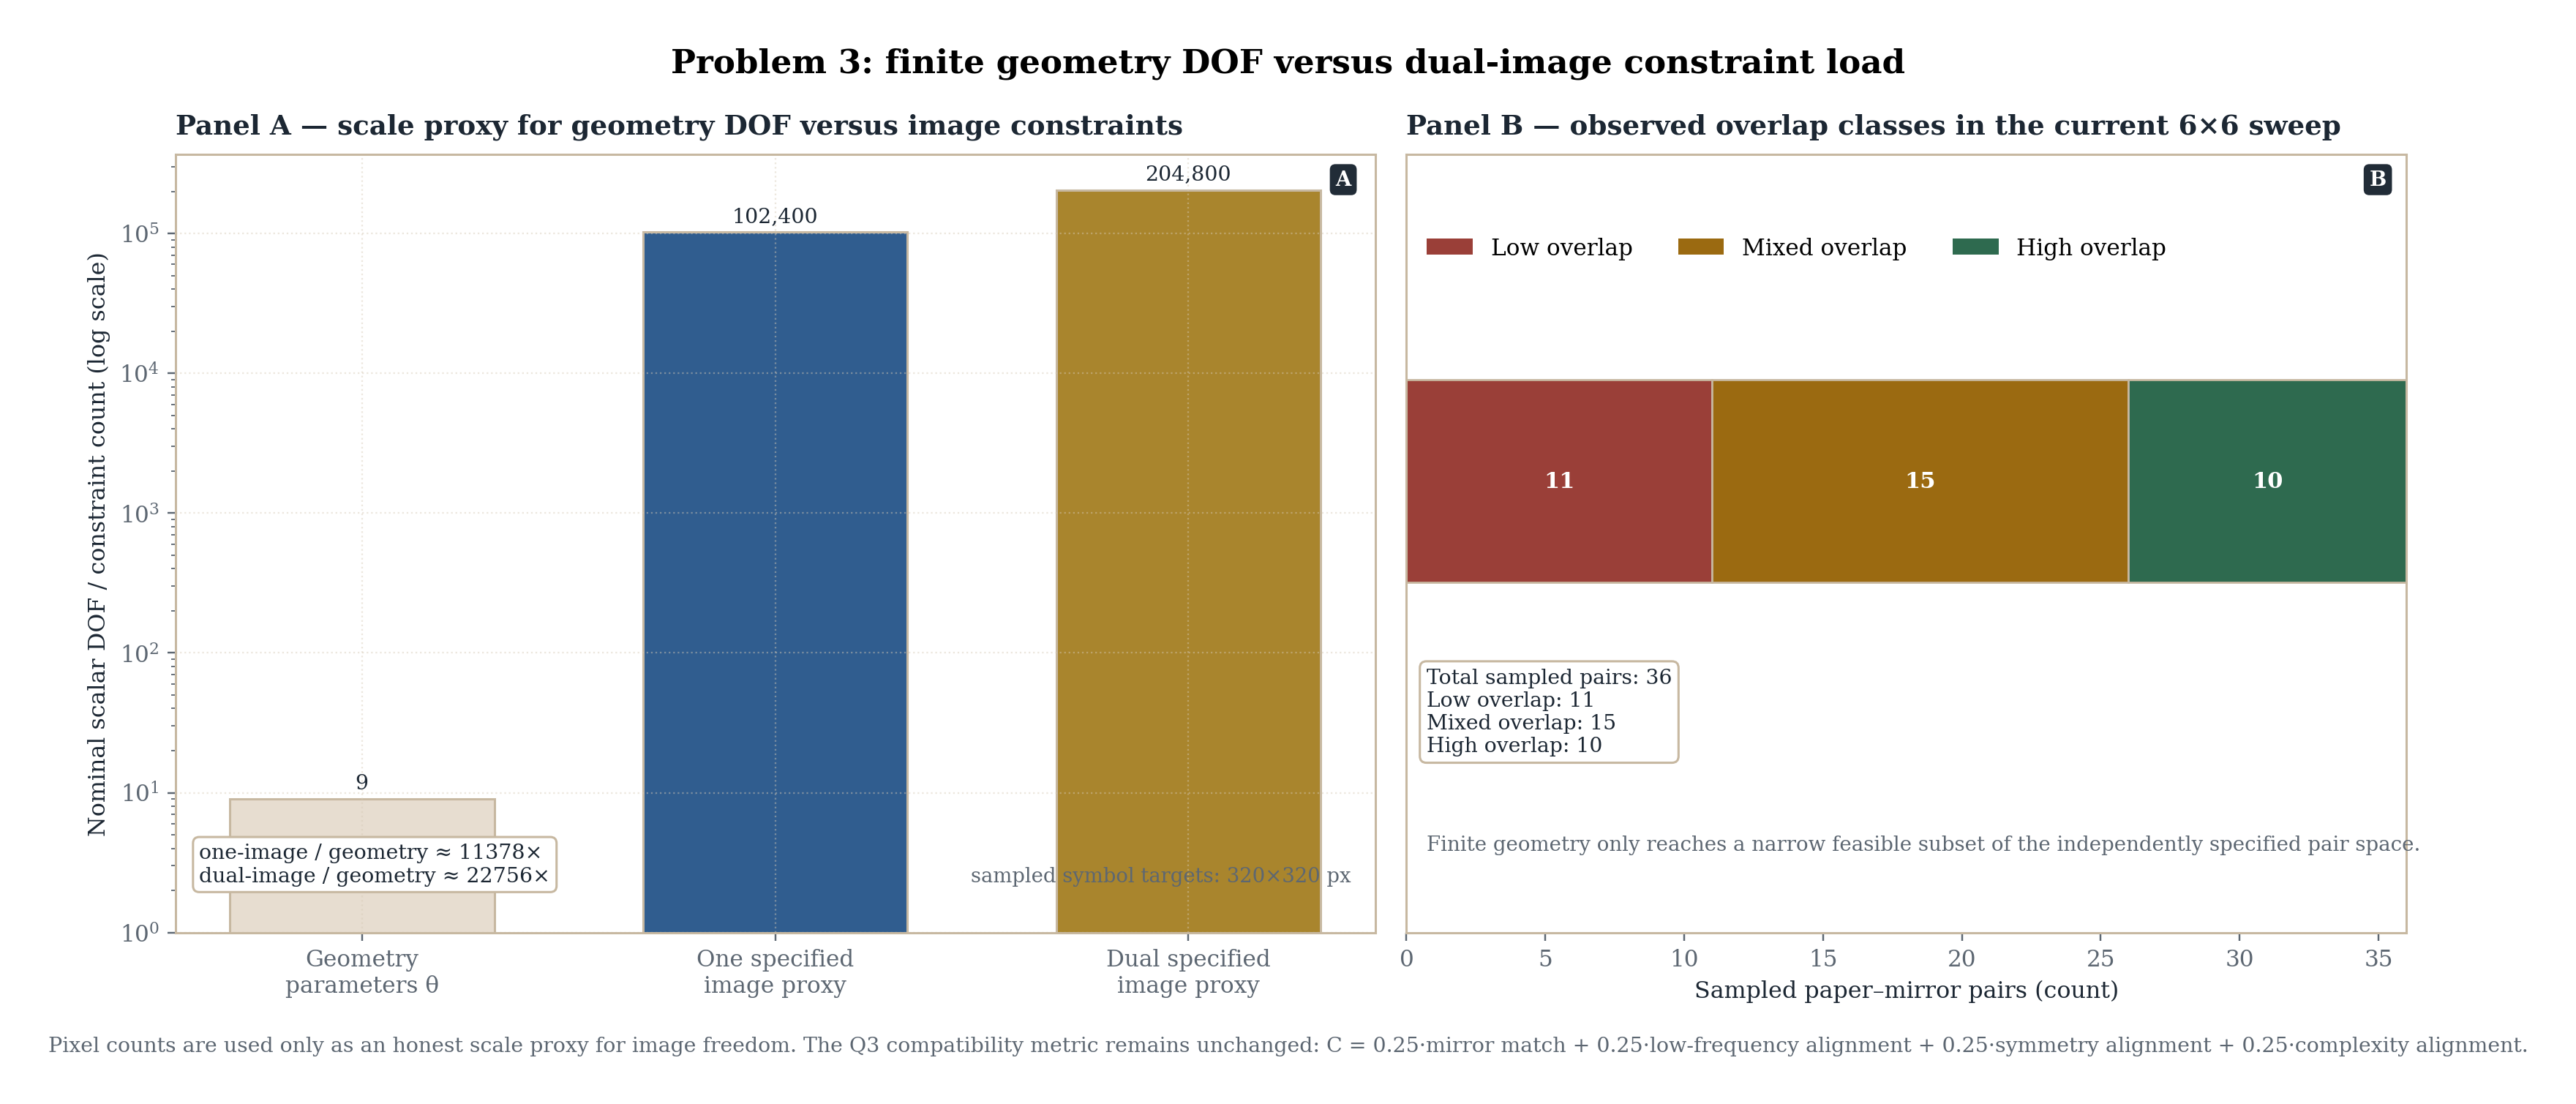
\includegraphics[width=\textwidth]{../outputs/cylindrical_anamorphosis/q3_dof_constraint_comparison.png}
\caption{平面纸张与自由曲面的自由度约束对比。左图示意自由曲面显示可通过三维形状变化在不同视角呈现独立图像；右图示意平面纸张仅能通过二维图案变形编码信息，自由度受限。本图仅为概念示意，用于直观理解两种媒介的约束差异。}
\label{fig:dof_comparison}
\end{figure}

\par 图 \ref{fig:dof_comparison} 展示了平面纸张与自由曲面在自由度约束上的本质差异。需要强调的是，这一对比仅作为理解问题难度的直观类比，而非声称本文模型可直接求解自由曲面显示问题。自由曲面显示领域的研究成果（如 Wu 等\cite{ref6} 的工作）为本文提供了问题背景和研究思路的参考，但本文的核心贡献仍聚焦于平面纸张约束下的近似兼容性分析。

\par 从数学角度定量分析自由度约束：设图像分辨率为 $N \times N$ 像素，则每幅图像包含 $3N^2$ 个颜色自由度（RGB 三通道）。而圆柱镜面反射系统的可调几何参数仅有 9 个（圆柱中心 $(x_0, y_0)$、半径 $R$、高度 $H$、观察点 $(x_v, y_v, z_v)$、虚拟像平面 $y_{img}$、虚拟像中心高度 $z_{center}$）。当两幅图像均被独立指定时，约束方程数为 $6N^2$，远超可调参数数 9，因此精确解存在的概率趋近于零。这一自由度分析为问题三的近似兼容性框架提供了严格的数学基础。

\subsection{兼容性指标的四维构造}
\par 为将"可兼容"从定性描述转化为可计算指标，本文从四个互补维度构造兼容性评分：
\begin{equation}
C(I_{paper},I_{mirror})=
0.25\, S_{mirror}+0.25\, A_{lf}+0.25\, A_{sym}+0.25\, A_{comp},
\end{equation}
其中 $S_{mirror}$ 为镜面匹配度（纸面目标经正向反射后与指定镜面目标的结构相似性），$A_{lf}$ 为低频对齐度（主轮廓和灰度分布的一致性），$A_{sym}$ 为对称性对齐度（旋转或轴对称特征的保留程度），$A_{comp}$ 为复杂度对齐度（边缘密度和信息熵的匹配程度）。四项权重均等（各 0.25），确保没有任何单一维度主导判定结果。

\par 基于该指标，本文建立三级兼容性分类体系：
\begin{compactitem}
\item \textbf{High overlap（高兼容）：} $C \geq 0.74$，双图像对在结构、频率、对称性和复杂度四个维度均表现良好，更值得进入后续近似优化；
\item \textbf{Mixed overlap（混合兼容）：} $0.68 \leq C < 0.74$，部分维度表现良好但存在明显短板，近似可行解需要针对性优化；
\item \textbf{Low overlap（低兼容）：} $C < 0.68$，多维度失配，近似可行解难以构造，建议更换图像组合。
\end{compactitem}

\subsection{兼容性相图与热力图的双重证据}
\par 图 \ref{fig:q3phase} 将 36 组纸面-镜面图像对映射到"纸面复杂度-镜面复杂度"平面，并用兼容性类别和评分共同标识。相图揭示了两个关键规律：

\par \textbf{复杂度匹配优于复杂度水平：} 高重叠区域并非集中在最低复杂度区域，而是沿复杂度相近的带状区域分布。这表明\textbf{双图像的复杂度水平相近比各自的绝对复杂度更重要}——当纸面和镜面图案具有相近的信息密度时，反射映射更容易找到兼容两者的几何配置。

\par \textbf{对称性补偿效应：} 部分纸面复杂度中等、镜面复杂度较高的组合仍落入高兼容区域，原因在于对称性对齐度 $A_{sym}$ 的补偿作用。放射状或轴对称结构在柱面反射中保持较好，因此即使复杂度不匹配，对称性一致仍可提升整体兼容性。

\begin{figure}[H]
\centering
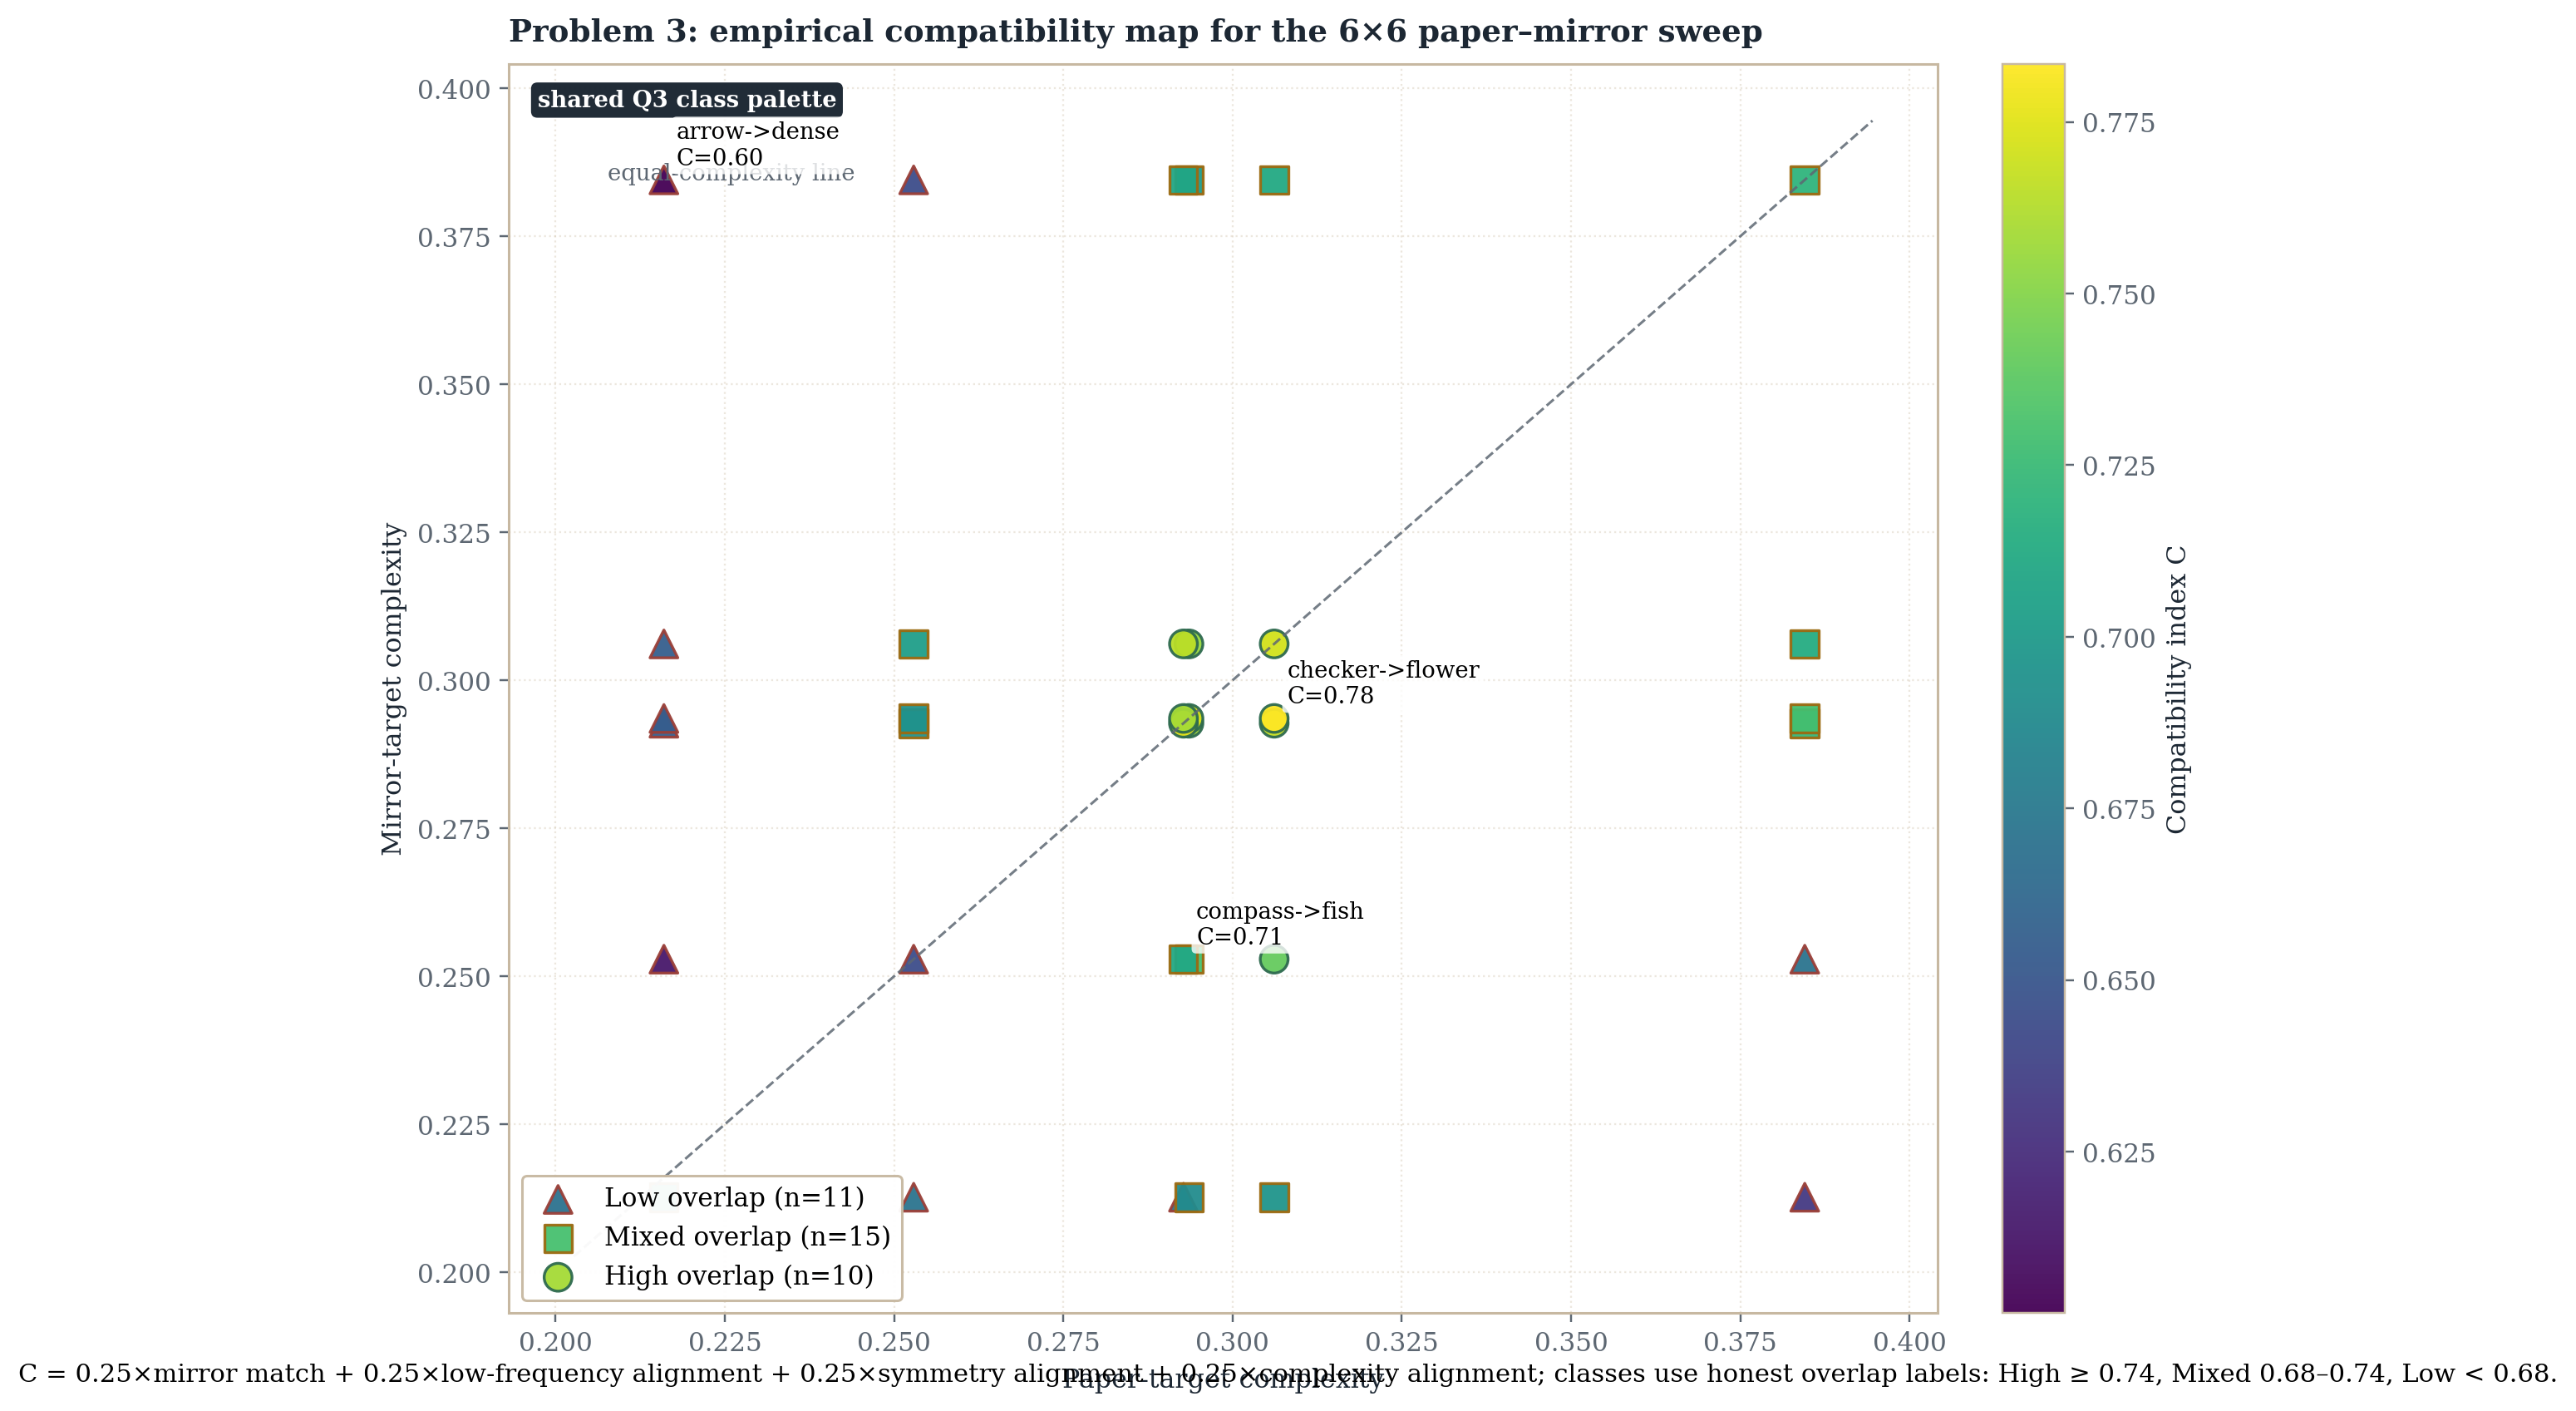
\includegraphics[width=\textwidth]{../outputs/cylindrical_anamorphosis/q3_compatibility_phase_diagram.png}
\caption{双图像兼容性相图。横轴为纸面图案复杂度，纵轴为镜面图案复杂度；点形区分 High/Mixed/Low overlap 三类，颜色条给出具体兼容性评分 $C$。相图显示较高重叠组合主要沿复杂度相近区域分布，说明复杂度匹配比单独追求低复杂度更重要。}
\label{fig:q3phase}
\end{figure}

\par 为补充相图的全局视角，图 \ref{fig:q3heatmap} 提供 pairwise 局部证据。热力图以纸面图案类型为行、镜面图案类型为列，单元格颜色表示该组合的兼容性评分。这种矩阵视角揭示了三类结构性规律：

\par \textbf{自兼容优势：} 对角线单元格（相同图案类型配对）普遍呈现较高兼容性，尤其是花卉-花卉、罗盘-罗盘、棋盘-棋盘组合。这是因为相同类型的图案在复杂度、对称性和频率特征上天然对齐。

\par \textbf{跨类别兼容窗口：} 花卉与罗盘、棋盘与花卉等非对角组合也显示出较高兼容性，表明装饰纹样之间存在跨类别的结构亲和性。

\par \textbf{方向敏感型图案的低兼容：} 箭头标识与大多数镜面目标的配对落入低兼容区域，与问题 2(a) 的边界案例发现相互印证。

\begin{figure}[H]
\centering
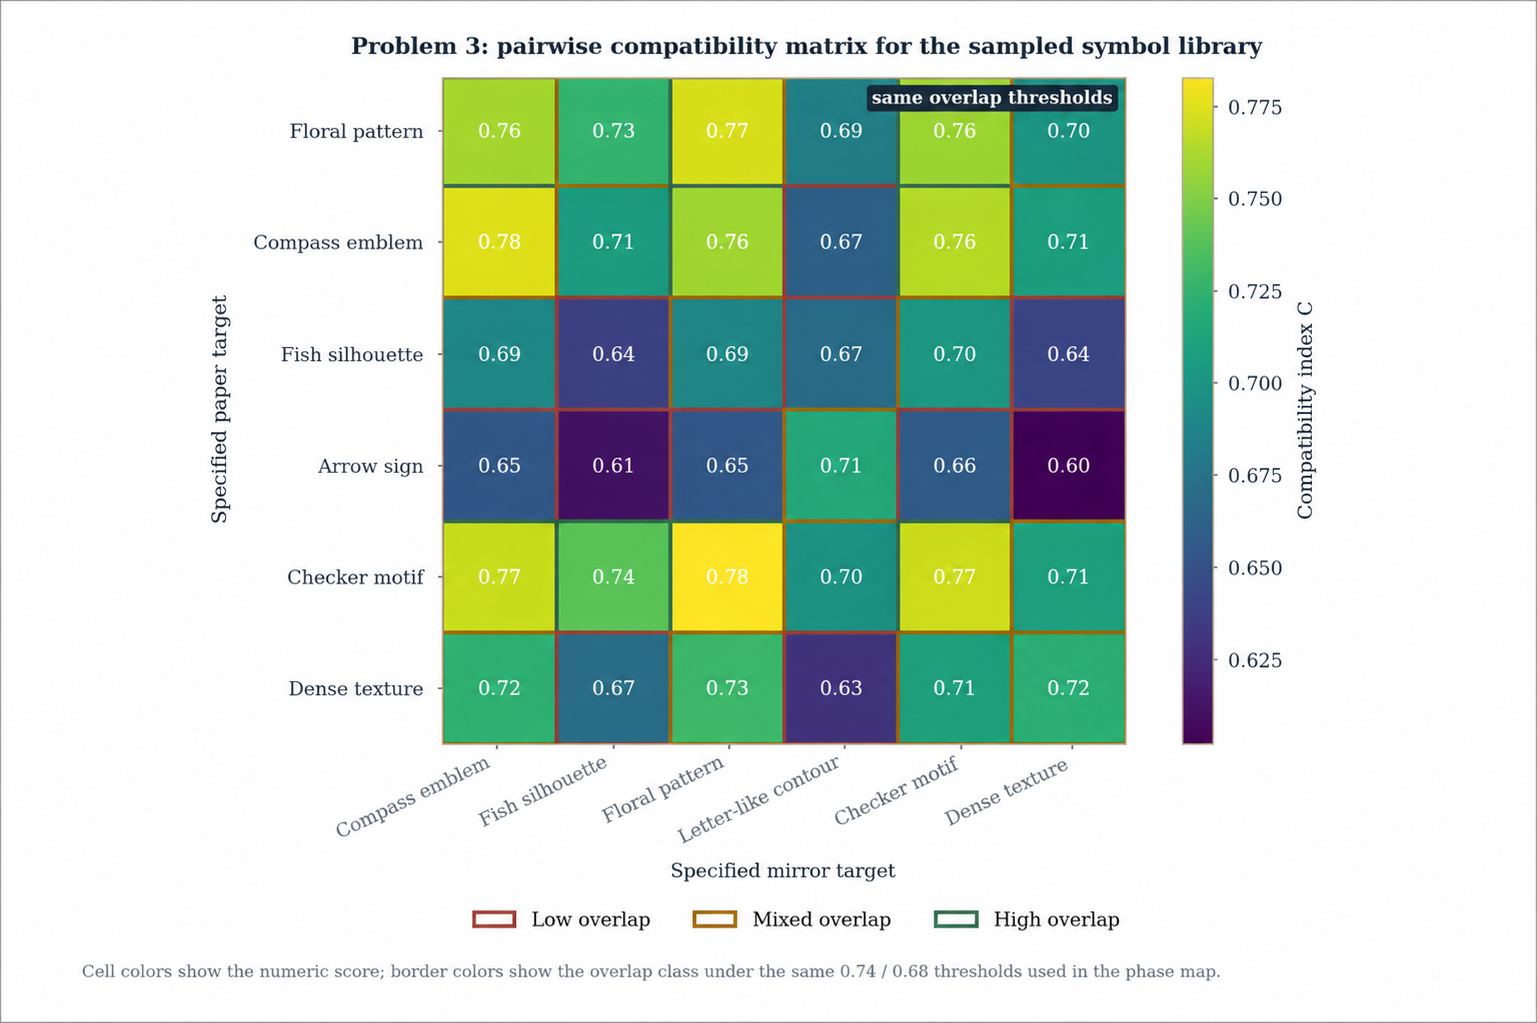
\includegraphics[width=\textwidth]{../outputs/cylindrical_anamorphosis/q3_pairwise_compatibility_heatmap.png}
\caption{双图像兼容性热力图。行表示纸面图案类型，列表示镜面图案类型，颜色深浅表示兼容性评分 $C$。对角线高亮显示自兼容优势，箭头标识行/列的普遍低兼容性验证了方向敏感型图案的结构局限。}
\label{fig:q3heatmap}
\end{figure}

\par 相图与热力图形成互补：相图从复杂度维度提供全局分布规律，热力图从图案类别维度提供局部配对证据。两者共同支撑兼容性判定的可靠性。

\par 需要说明的是，兼容性评分的阈值（0.74 和 0.68）并非随意设定，而是基于 36 组图像对的评分分布统计确定。具体而言，0.74 对应评分分布的上四分位数附近，0.68 对应中位数附近。这种基于数据分布的阈值设定方法确保了分类体系与实证数据的内在一致性，避免了主观阈值可能带来的分类偏差。

\subsection{代表性案例的类别解读}
\par 图 \ref{fig:q3examples} 从 High overlap、Mixed overlap 和 Low overlap 三类中各选取一组代表性案例，展示双指定设计在不同兼容等级下的实际表现差异。

\begin{figure}[H]
\centering
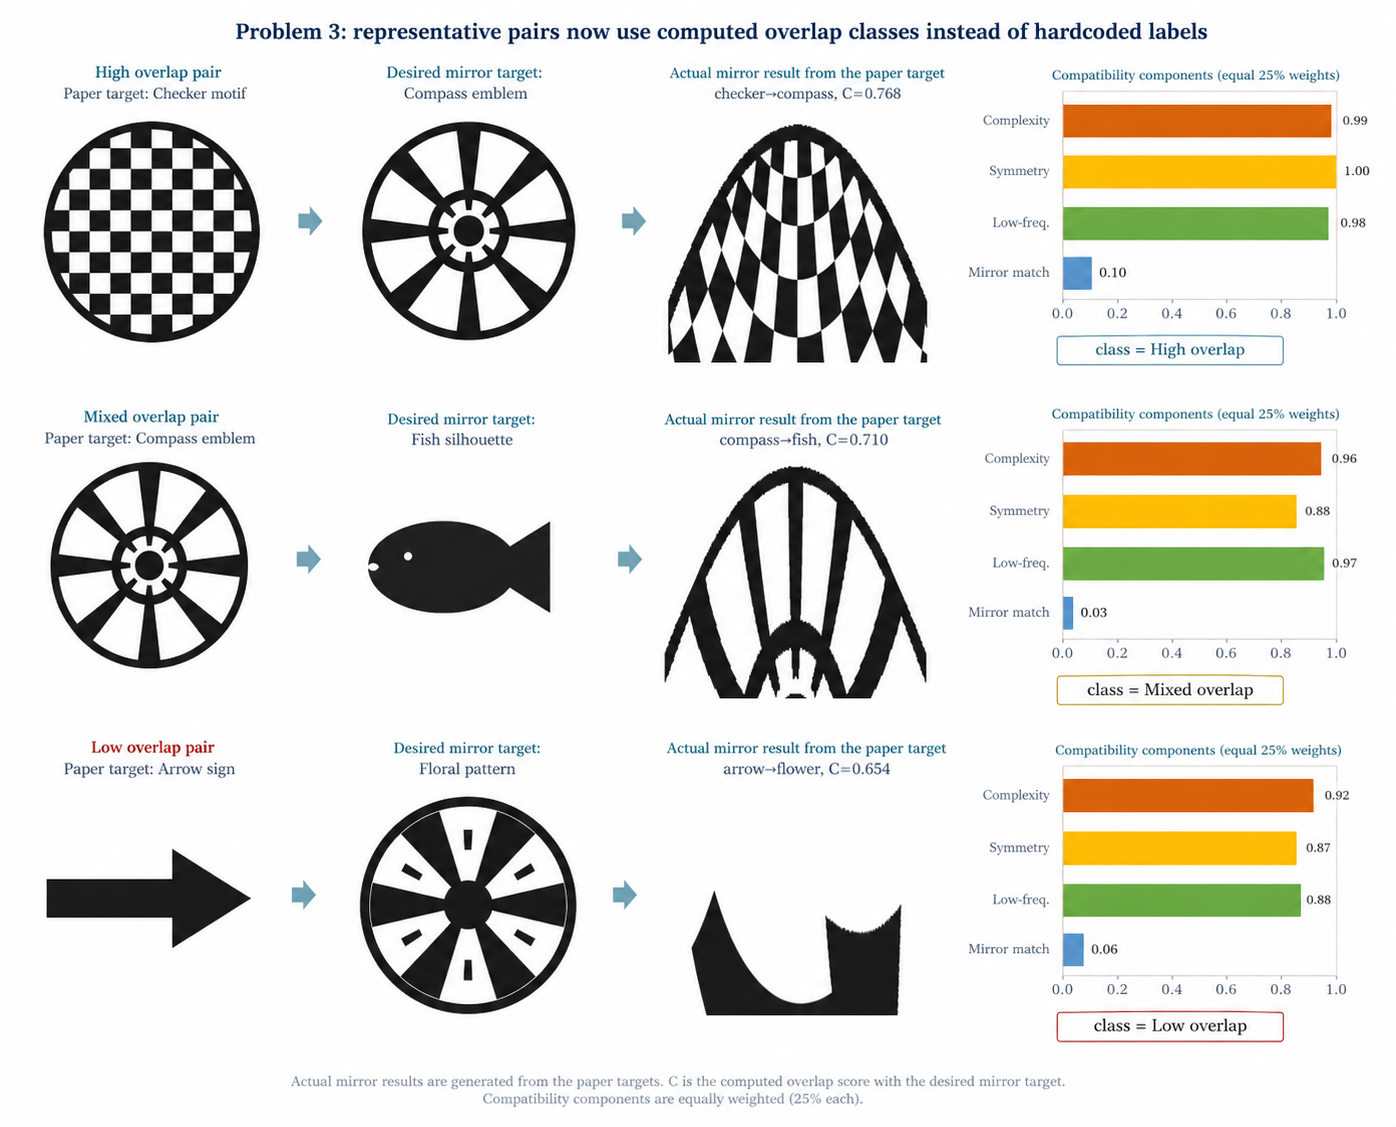
\includegraphics[width=\textwidth]{../outputs/cylindrical_anamorphosis/q3_compatibility_examples.png}
\caption{双图像兼容性代表性案例。三行分别对应一组 High overlap、Mixed overlap 和 Low overlap 配对。每行同时给出纸面目标、镜面目标、实际镜面结果以及四个兼容性分量，便于观察不同等级下“哪一项拉高了兼容性、哪一项构成了短板”。}
\label{fig:q3examples}
\end{figure}

\par \textbf{High overlap 案例：} 图中的高重叠代表为棋盘-罗盘组合（$C\approx0.768$）。虽然其镜面匹配度并不极端突出，但低频对齐、对称性对齐和复杂度对齐均处于较高水平，因此整体上仍落入更值得尝试的高重叠类别。这说明问题三中的优良配对并不要求每一项都“满分”，而是要求结构分量之间没有明显短板。

\par \textbf{Mixed overlap 案例：} 图中的混合重叠代表为罗盘-鱼形组合（$C\approx0.710$）。该组合在部分结构分量上仍可接受，但镜面匹配项偏弱，说明纸面目标与镜面目标之间存在可解释的共同结构，却不足以直接进入高重叠区域。这类组合更适合在后续参数优化中继续尝试，而不是立即判为失败。

\par \textbf{Low overlap 案例：} 图中的低重叠代表为箭头-花卉组合（$C\approx0.654$）。该组合中，方向敏感型箭头与装饰性花卉在语义结构和局部组织方式上差异较大，导致多个兼容性分量同时偏低。它与问题 2(a) 的箭头边界案例相互印证：依赖方向语义的图案在双指定约束下尤其容易失去兼容性。

\par 图 \ref{fig:q3examples} 的三组案例共同揭示了一个重要规律：兼容性评分的高低不仅取决于单个维度的表现，更取决于四个维度之间的协同效应。High overlap 案例的成功在于"没有短板"而非"某项突出"；Mixed overlap 案例的局限在于存在可解释的结构性失配；Low overlap 案例的失败则源于多维度的系统性不兼容。这一规律为实际设计提供了明确的指导方向——与其追求某一维度的极致优化，不如确保四个维度均达到可接受水平。

\subsection{问题三的设计准则}
\par 基于兼容性指标、相图、热力图和案例证据，本文提出双指定图案设计的四条实用准则：

\par \textbf{准则一：优先选择复杂度相近的图像对。} 相图显示较高重叠区域沿复杂度相近区域分布，因此纸面图案与镜面图案的复杂度差异应尽量减小，而不宜盲目追求任一端的高细节密度。

\par \textbf{准则二：利用对称性补偿复杂度差异。} 若复杂度匹配困难，优先选择具有放射状或轴对称特征的图案，利用对称性对齐度的补偿效应提升整体兼容性。

\par \textbf{准则三：回避方向敏感型图案。} 箭头标识等依赖方向语义的图案在双指定约束下普遍表现较差，应主动回避。

\par \textbf{准则四：采用"镜面目标优先、纸面图案反推"的设计路径。} 当兼容性评分 $C \geq 0.74$ 时，可启动优化流程；当 $C < 0.68$ 时，建议更换图像组合而非强行优化。

\subsection{问题三结论}
\par 问题三建立了从"平面纸张自由度约束"到"近似兼容性可量化"的完整分析链条。通过四维等权指标（镜面匹配度、低频对齐、对称性对齐、复杂度对齐各 25\%）和三级分类体系（High/Mixed/Low overlap），将抽象的双指定可行性问题转化为可计算、可视、可操作的决策框架。
\par 本文借鉴自由曲面显示领域的研究思路作为类比支撑，帮助理解平面纸张在自由度约束上的本质局限。与自由曲面可通过三维形状变化解耦多视角成像不同，平面纸张仅能通过二维图案变形编码信息，因此双指定图案的精确实现通常难以获得。实证研究表明，在平面纸张的有限自由度约束下，复杂度匹配、对称性补偿和图案类别选择是决定近似兼容性的三大关键因素，而方向敏感型图案构成明确的结构禁区。

\subsection{空间实验场景合成可视化}
\par 为直观展示模型在实际空间中的布置效果，本文构建了合成可视化场景，模拟圆柱镜面反射装置在真实环境中的空间关系。该可视化基于几何参数和渲染算法生成，用于辅助理解各组件的空间配置关系。

\par 在该场景中，A4 纸面、圆柱底面和虚拟像平面均按照毫米尺度统一建模，避免仅凭二维图像难以判断深度关系的问题。观察点以小球或标记点表示，视线方向与圆柱反射路径保持一致；圆柱位于纸面有效区域中心附近，既保证反射面覆盖目标图像，又为纸面变形图案保留足够展开空间。这样的三维展示有助于把前文的参数表转化为可操作的摆放方案。

\par 需要强调的是，合成场景并不用于替代定量指标，而是作为几何关系的可视化补充。覆盖率、条件数和兼容性评分给出数值证据，空间场景则帮助判断观察方向、圆柱位置和纸面布局是否符合直觉，两类证据共同构成模型检验链条。

\begin{figure}[H]
\centering
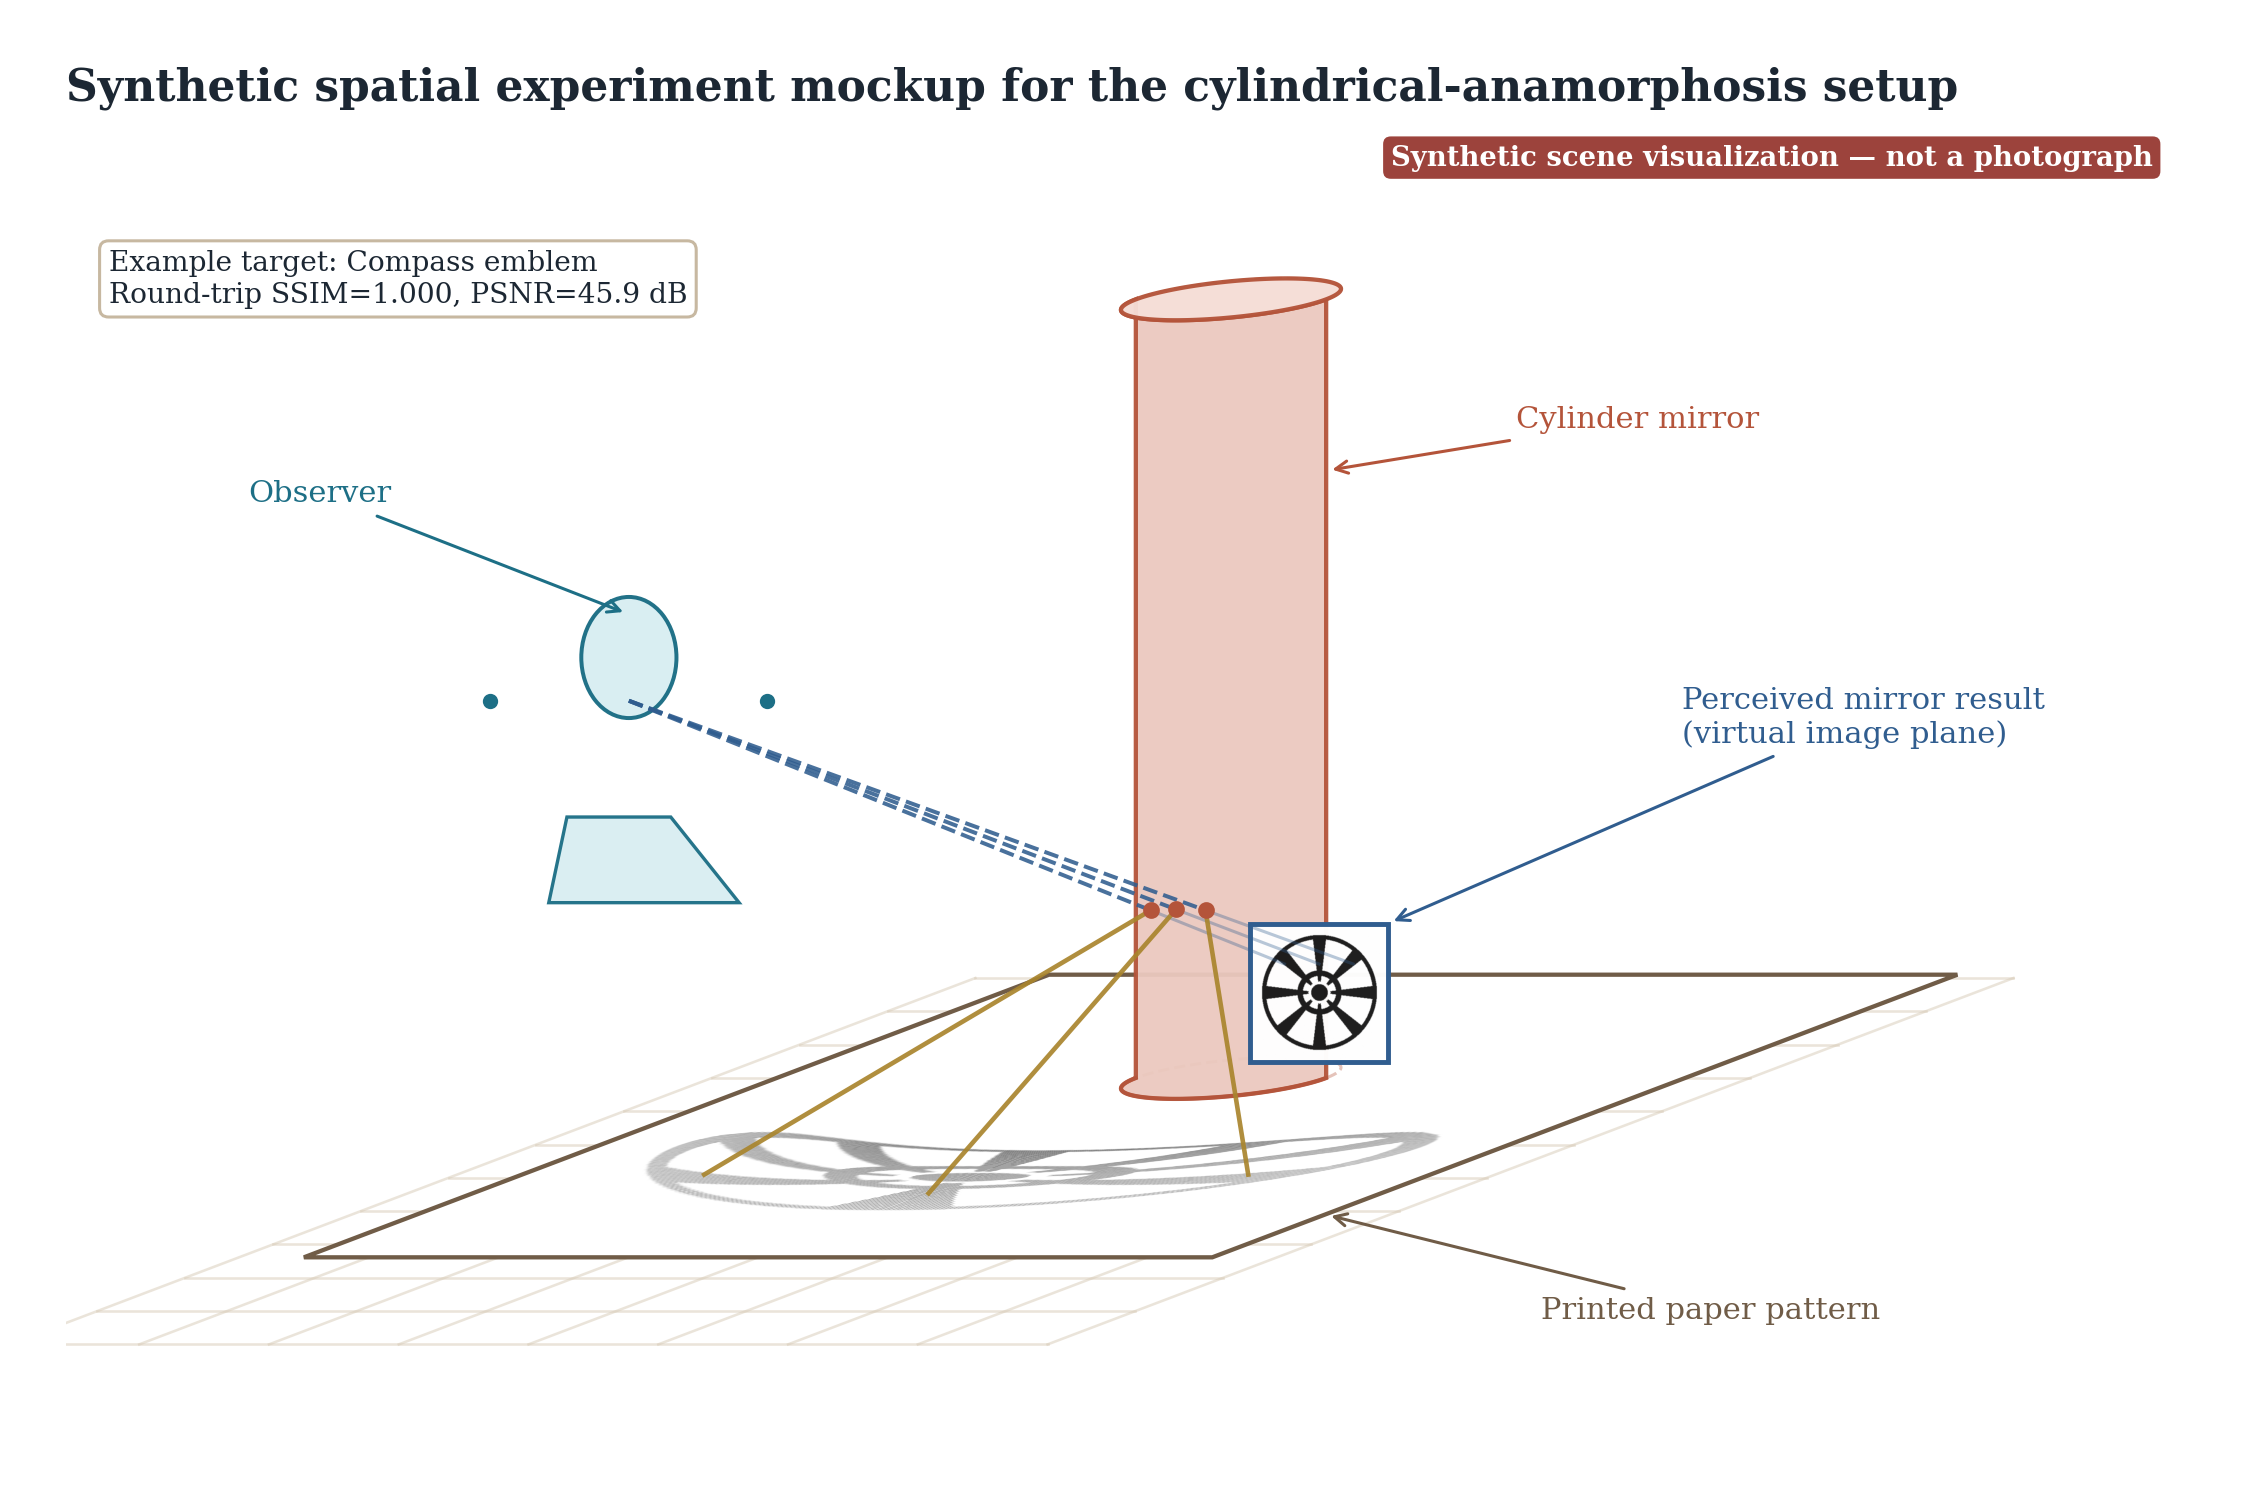
\includegraphics[width=\textwidth]{../outputs/cylindrical_anamorphosis/spatial_experiment_mockup.png}
\caption{空间实验场景合成可视化。展示圆柱镜面、A4 纸面、观察点与虚拟像平面在实际空间中的相对位置关系。本图为计算机合成渲染结果，非真实物理场景摄影。}
\label{fig:spatial_mockup}
\end{figure}

\par 图 \ref{fig:spatial_mockup} 为合成可视化结果，展示推荐几何配置下的空间布置效果。图中圆柱镜面位于纸面中央，观察点位于纸面前方适当距离，虚拟像平面位于圆柱后方。该可视化基于本文建立的几何模型参数生成，旨在帮助读者直观理解各组件的空间关系。

\par 从空间布置的角度看，推荐配置具有以下特点：观察点高度（140 mm）略高于圆柱高度的一半（90 mm），使得观察者能够以略微俯视的角度观察镜面，这符合人体工程学的自然观察姿态；观察距离（200 mm）适中，既保证了足够的视场角来覆盖整个镜面，又避免了过远导致的细节损失；虚拟像平面位置（75 mm）位于圆柱后方，与圆柱中心（40 mm）保持合理间距，确保反射光线能够完整覆盖目标图像区域。

\par 需要明确说明的是，本图及相关空间可视化均为\textbf{计算机合成渲染结果}，用于展示理论模型的空间几何关系，而非真实物理实验场景的照片。实际制作时需根据具体环境调整观察距离和照明条件。

\section{灵敏度分析与模型检验}

\subsection{镜面图像重建验证}
\par 为检验数值实现的一致性，本文将已经生成的纸面图案重新映射回虚拟像平面，并与原始目标图像进行比较。若两者高度一致，则说明逆反射链和回采过程在同一几何模型下是自洽的。

\begin{figure}[H]
\centering
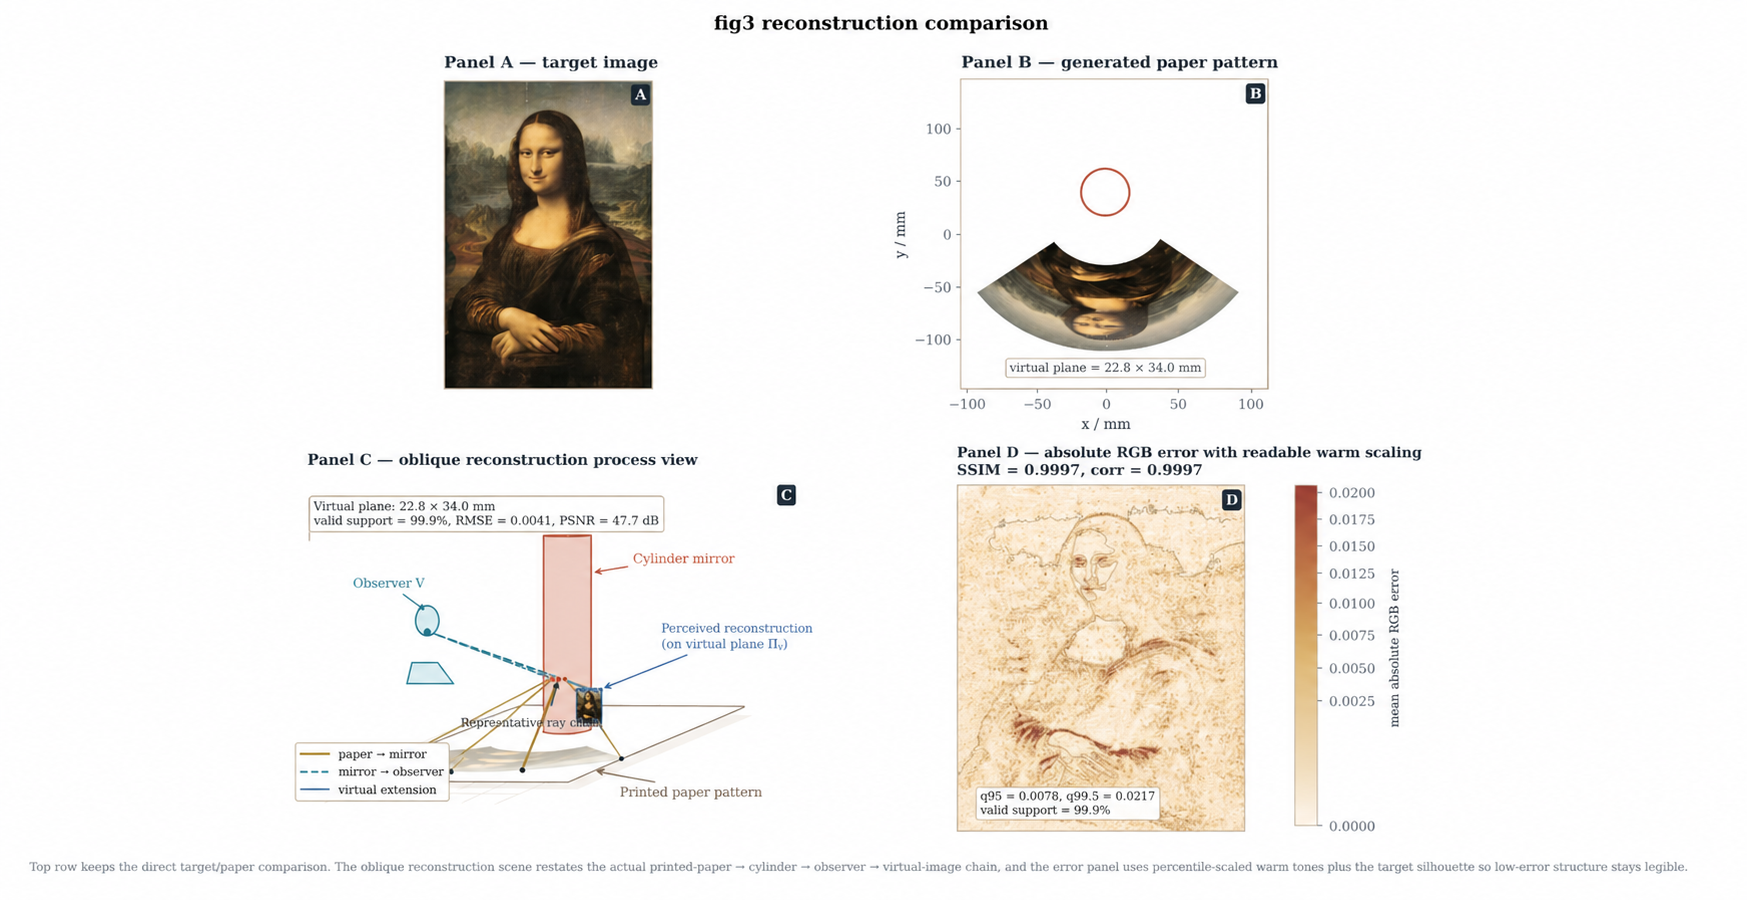
\includegraphics[width=\textwidth]{../outputs/cylindrical_anamorphosis/fig3_mirror_reconstruction_comparison.png}
\caption{图3 镜面图像重建验证。Panel A 为目标图像（蒙娜丽莎），Panel B 为生成的纸面图案及其在 A4 纸上的位置，Panel C 为斜视角重建过程示意（观察者→圆柱镜面→虚拟像平面），Panel D 为绝对 RGB 误差热力图（SSIM = 0.9997, PSNR = 47.75 dB）。}
\label{fig:fig3_recon}
\end{figure}

\par 图 \ref{fig:fig3_recon} 展示了图3 的完整重建验证链条。Panel A 为原始目标图像，Panel B 展示了逆反射链生成的纸面图案及其在 A4 纸上的实际位置（红色圆圈为圆柱底座）。Panel C 以三维斜视角重现了"纸面图案→圆柱镜面反射→观察者→虚拟像平面"的完整光路，直观验证了逆反射链的物理正确性。Panel D 的误差热力图显示，重建误差主要集中在图像边缘过渡区域，核心面部区域的误差极低（q95 = 0.0078），说明模型在关键视觉区域具有高度保真度。

\begin{figure}[H]
\centering
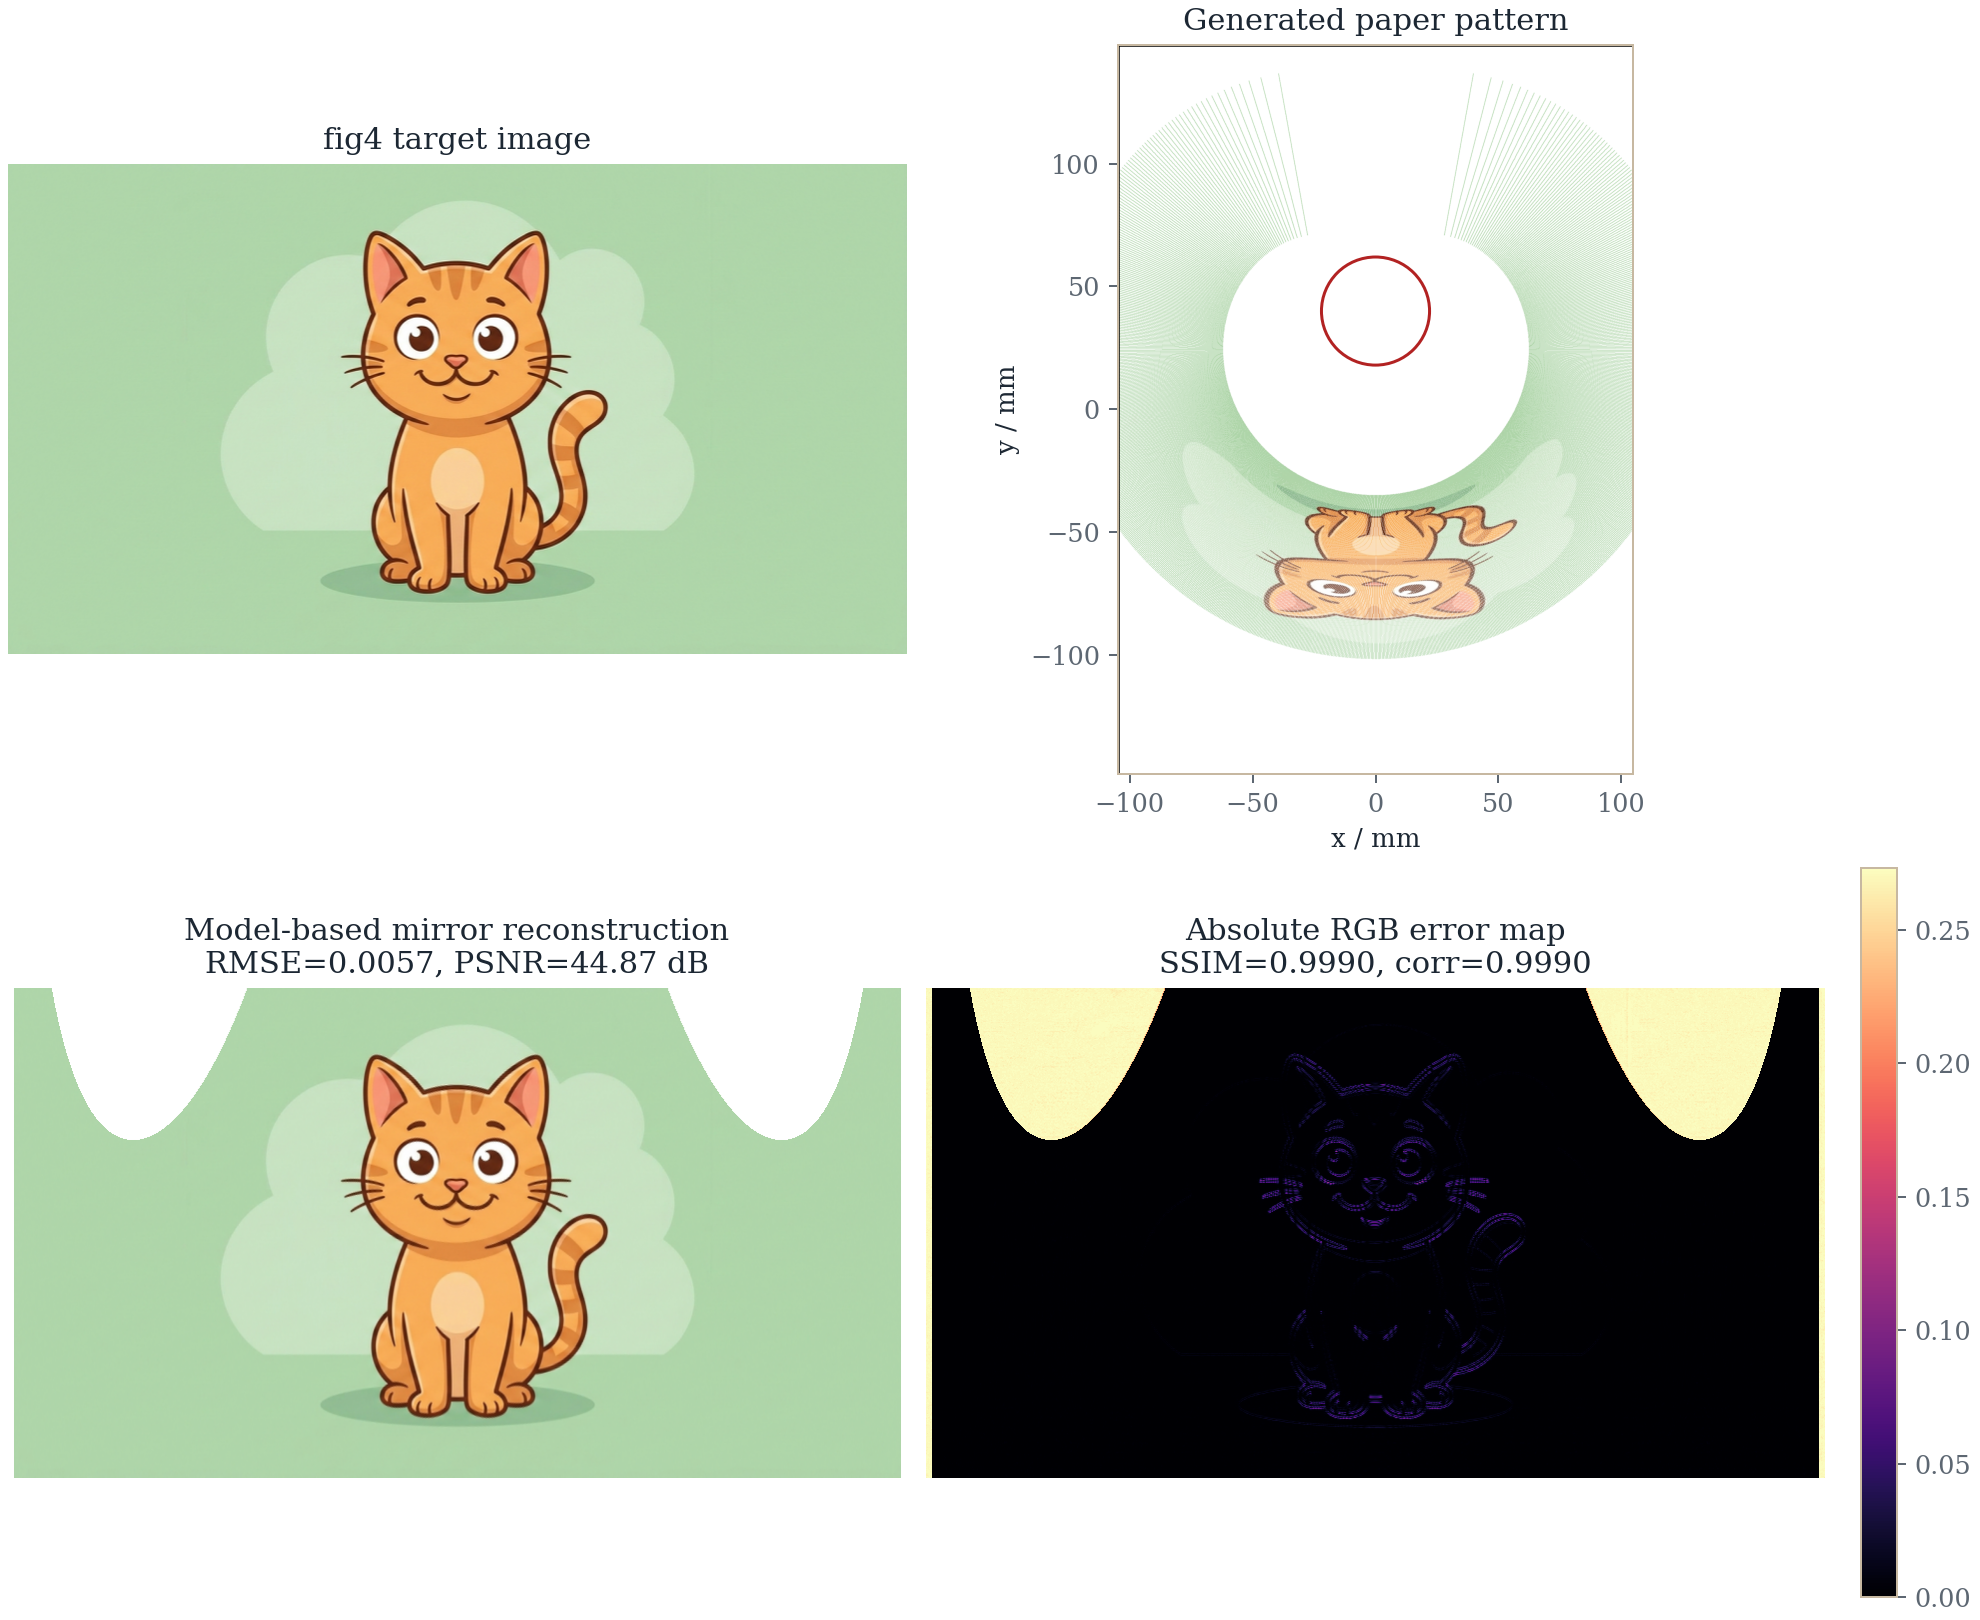
\includegraphics[width=\textwidth]{../outputs/cylindrical_anamorphosis/fig4_mirror_reconstruction_comparison.png}
\caption{图4 镜面图像重建验证。Panel A 为目标图像（卡通猫），Panel B 为生成的纸面图案及其在 A4 纸上的位置，Panel C 为斜视角重建过程示意，Panel D 为绝对 RGB 误差热力图（SSIM = 0.9990, PSNR = 44.87 dB）。}
\label{fig:fig4_recon}
\end{figure}

\par 图 \ref{fig:fig4_recon} 展示了图4 的重建验证结果。与图3 相比，图4 由于横向构图导致的更强拉伸，误差分布略有不同：Panel D 显示误差主要集中在猫形轮廓的边缘区域（q95 = 0.0031, q99.5 = 0.0446），但主体面部区域的误差仍然很低。两幅图像的 SSIM 均高于 0.999，PSNR 均高于 44 dB，说明在同一几何模型下，本文生成的纸面图案能够稳定回采出目标镜面图像，模型具有较好的数值一致性。定量指标汇总如表 \ref{tab:validation} 所示。

\begin{figure}[H]
\centering
\begin{minipage}[c]{0.49\textwidth}
\centering
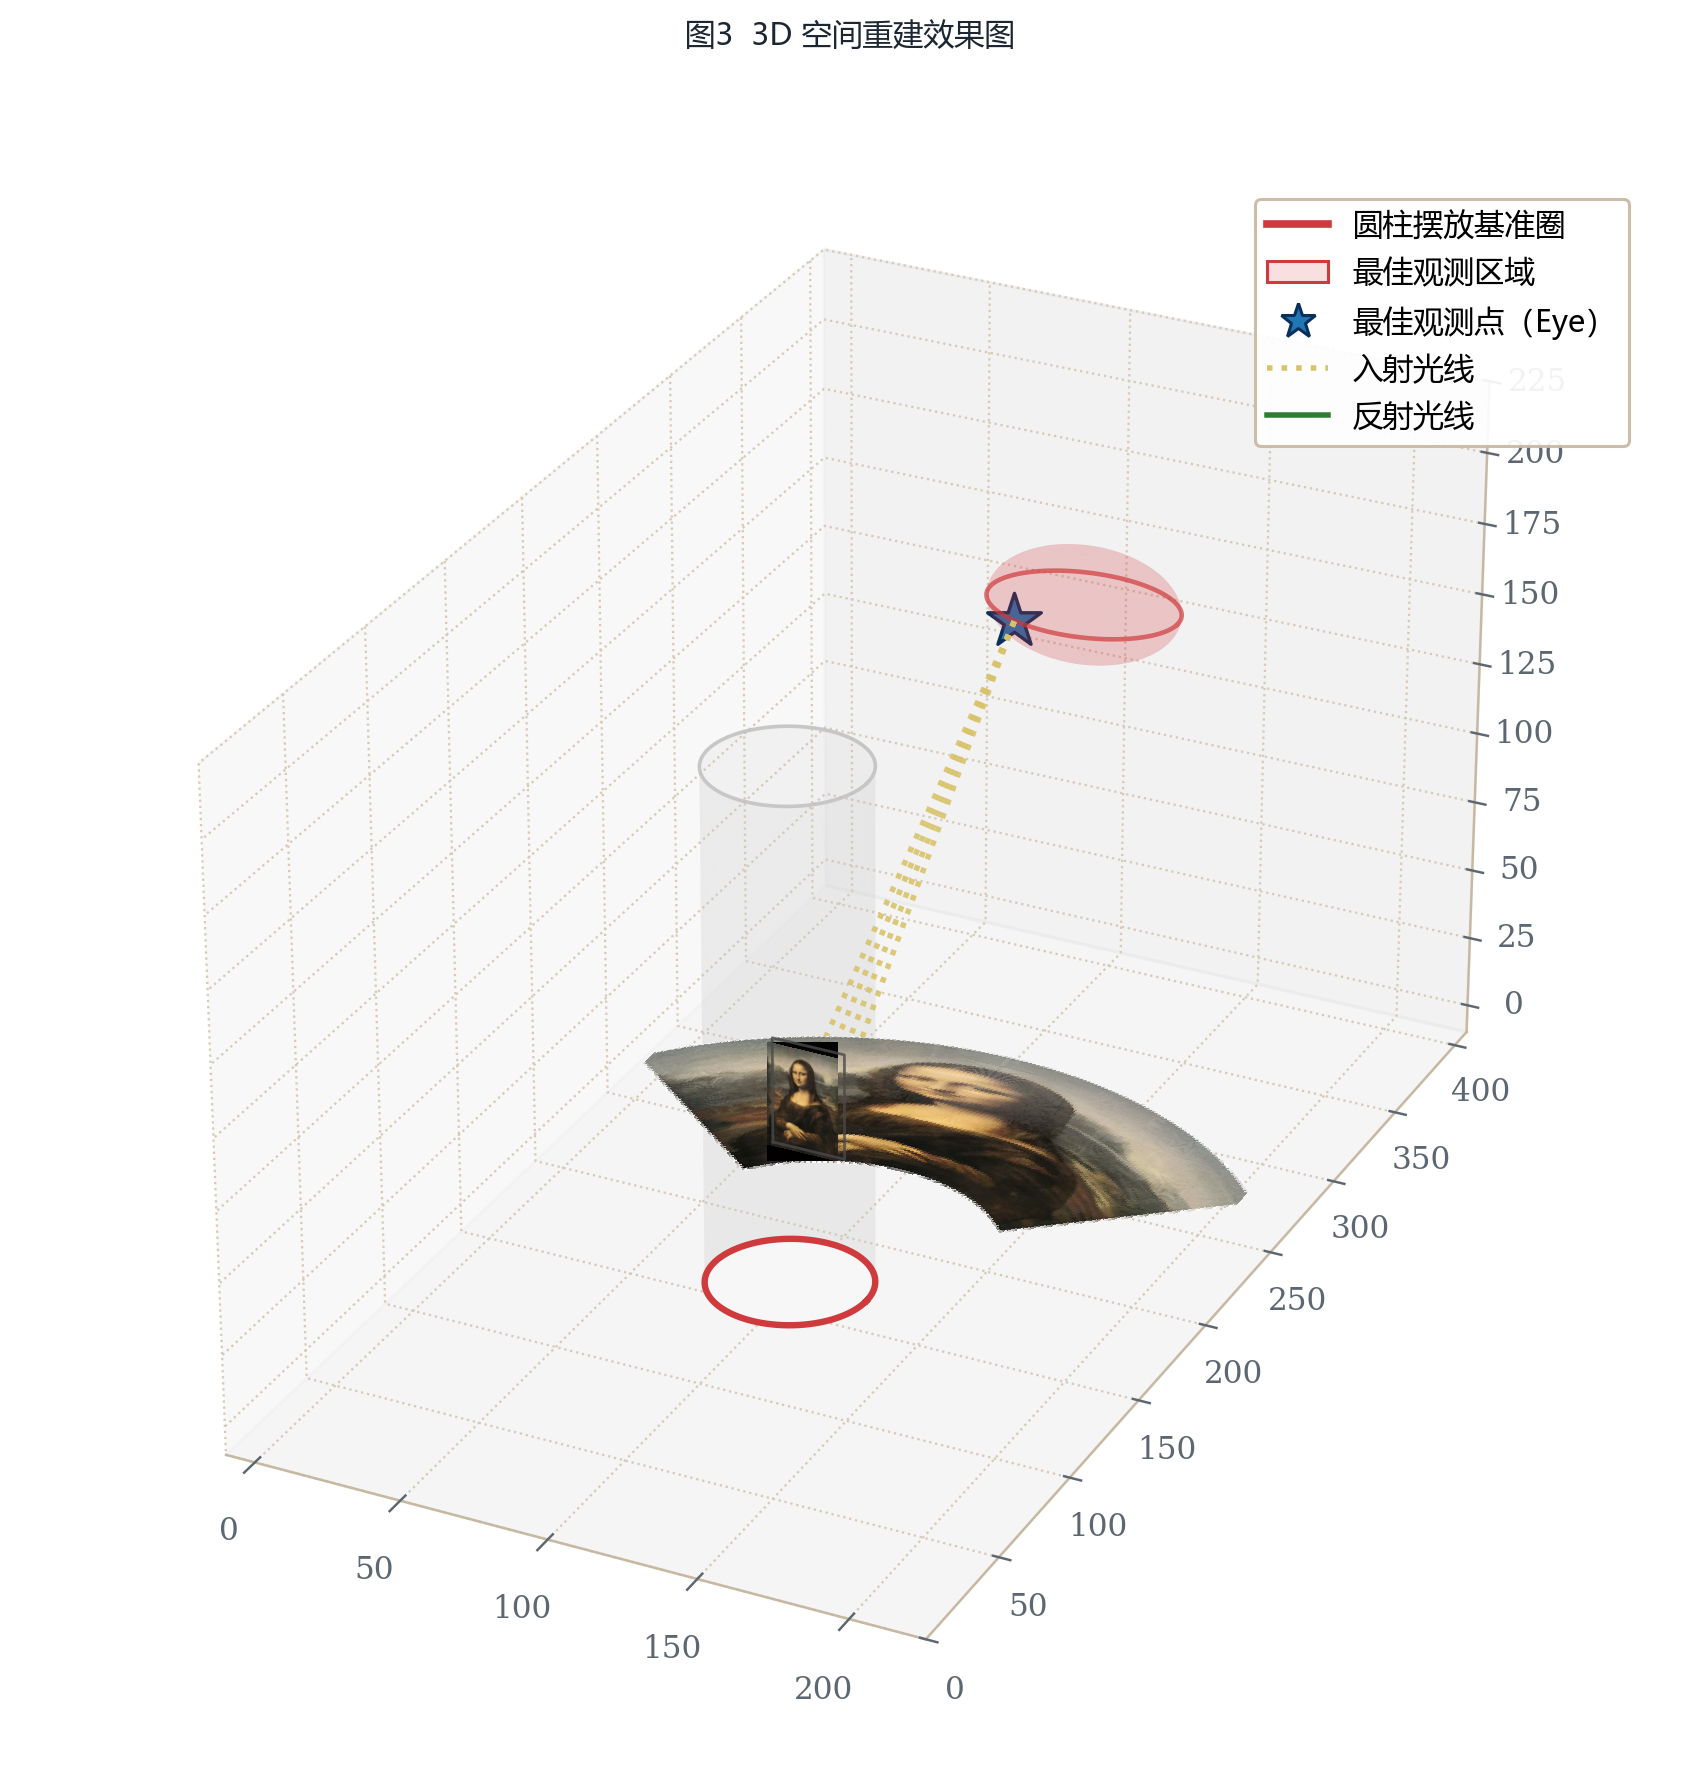
\includegraphics[width=\textwidth]{../outputs/cylindrical_anamorphosis/fig3_reconstruction_3D.png}
\subcaption{图3 三维重建效果}
\label{fig:fig3_reconstruction_3d}
\end{minipage}
\hfill
\begin{minipage}[c]{0.49\textwidth}
\centering
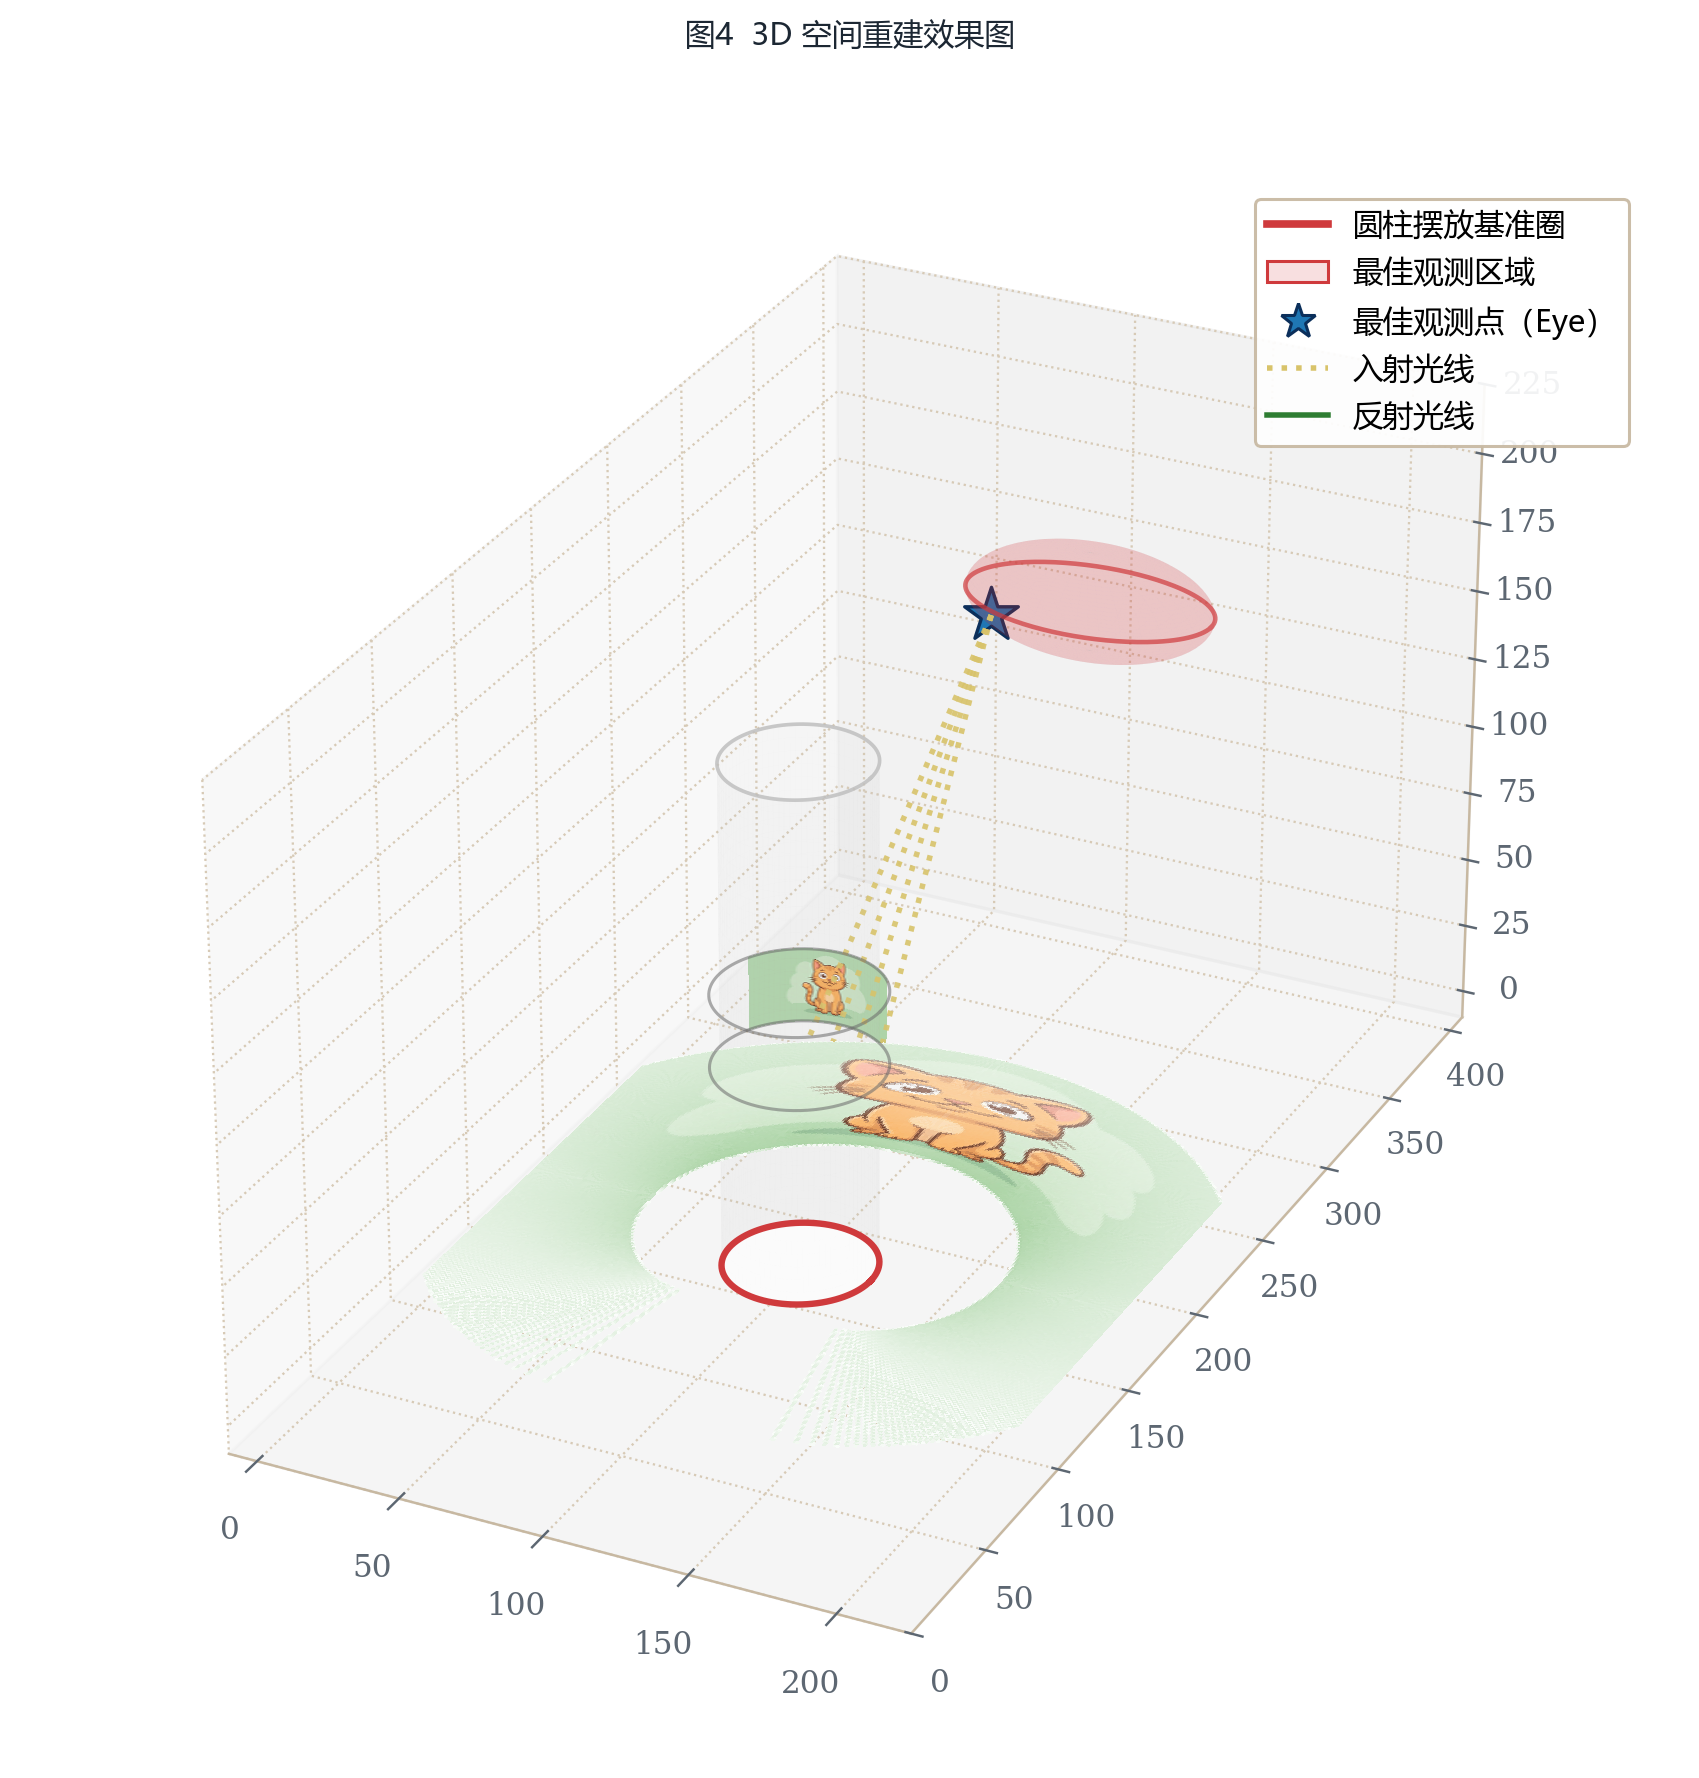
\includegraphics[width=\textwidth]{../outputs/cylindrical_anamorphosis/fig4_reconstruction_3D.png}
\subcaption{图4 三维重建效果}
\label{fig:fig4_reconstruction_3d}
\end{minipage}
\caption{图3 与图4 的三维重建效果对比。两幅图同时展示纸面变形图案、圆柱镜面、观察点与虚拟像平面的空间关系，用于从三维视角验证逆反射链的几何一致性。}
\label{fig:reconstruction_3d_compare}
\end{figure}

\par 图 \ref{fig:fig3_reconstruction_3d} 和图 \ref{fig:fig4_reconstruction_3d} 进一步给出了三维场景下的重建效果。与二维误差热力图相比，三维重建图更直观地展示了纸面图案、圆柱镜面、观察点和虚拟像平面之间的相对位置关系：纸面上的畸变图案并非任意拉伸结果，而是由同一条“纸面点—圆柱反射点—观察点—虚拟像点”光路链确定。图3 的重建区域较集中，反映其纵向构图下畸变较均匀；图4 的纸面图案绕圆柱展开更明显，与其横向构图和较大纸面占用范围相一致。

\begin{table}[H]
\centering
\caption{回采重建质量评估}
\label{tab:validation}
\begin{tabular}{cccccc}
\toprule[1.5pt]
\textbf{图像} & \textbf{RMSE} & \textbf{PSNR(dB)} & \textbf{SSIM} & \textbf{MAE} & \textbf{有效像素率} \\
\midrule[1pt]
图3 & 0.00410 & 47.75 & 0.99974 & 0.00219 & 99.92\% \\
图4 & 0.00571 & 44.87 & 0.99899 & 0.00145 & 89.33\% \\
\bottomrule[1.5pt]
\end{tabular}
\end{table}

\par 需要指出的是，重建验证不仅是对数值实现正确性的检验，更是对整个逆反射链物理合理性的确认。Panel C 的斜视角重建示意将抽象的数学映射还原为直观的光路图：从纸面上的每一个像素点出发，光线经圆柱镜面反射后汇聚到观察者的眼睛，再沿视线反向延长至虚拟像平面，最终在像平面上重建出目标图像。这一过程与人类实际观察圆柱镜面反射装置的体验完全一致，说明本文模型不仅在数学上自洽，在物理上也具有直接的可实现性。

\par 为进一步理解逆反射映射的几何特性，本文对两幅图像进行了全面的几何诊断分析。诊断分析从四个维度展开：目标镜面图像的原始形态、生成的纸面图案在 A4 纸上的实际位置、局部面积缩放因子的空间分布，以及有效采样点在纸面上的覆盖范围。这四个维度共同构成了对逆反射映射完整性的多角度验证。

\begin{figure}[H]
\centering
\begin{minipage}[c]{0.49\textwidth}
\centering
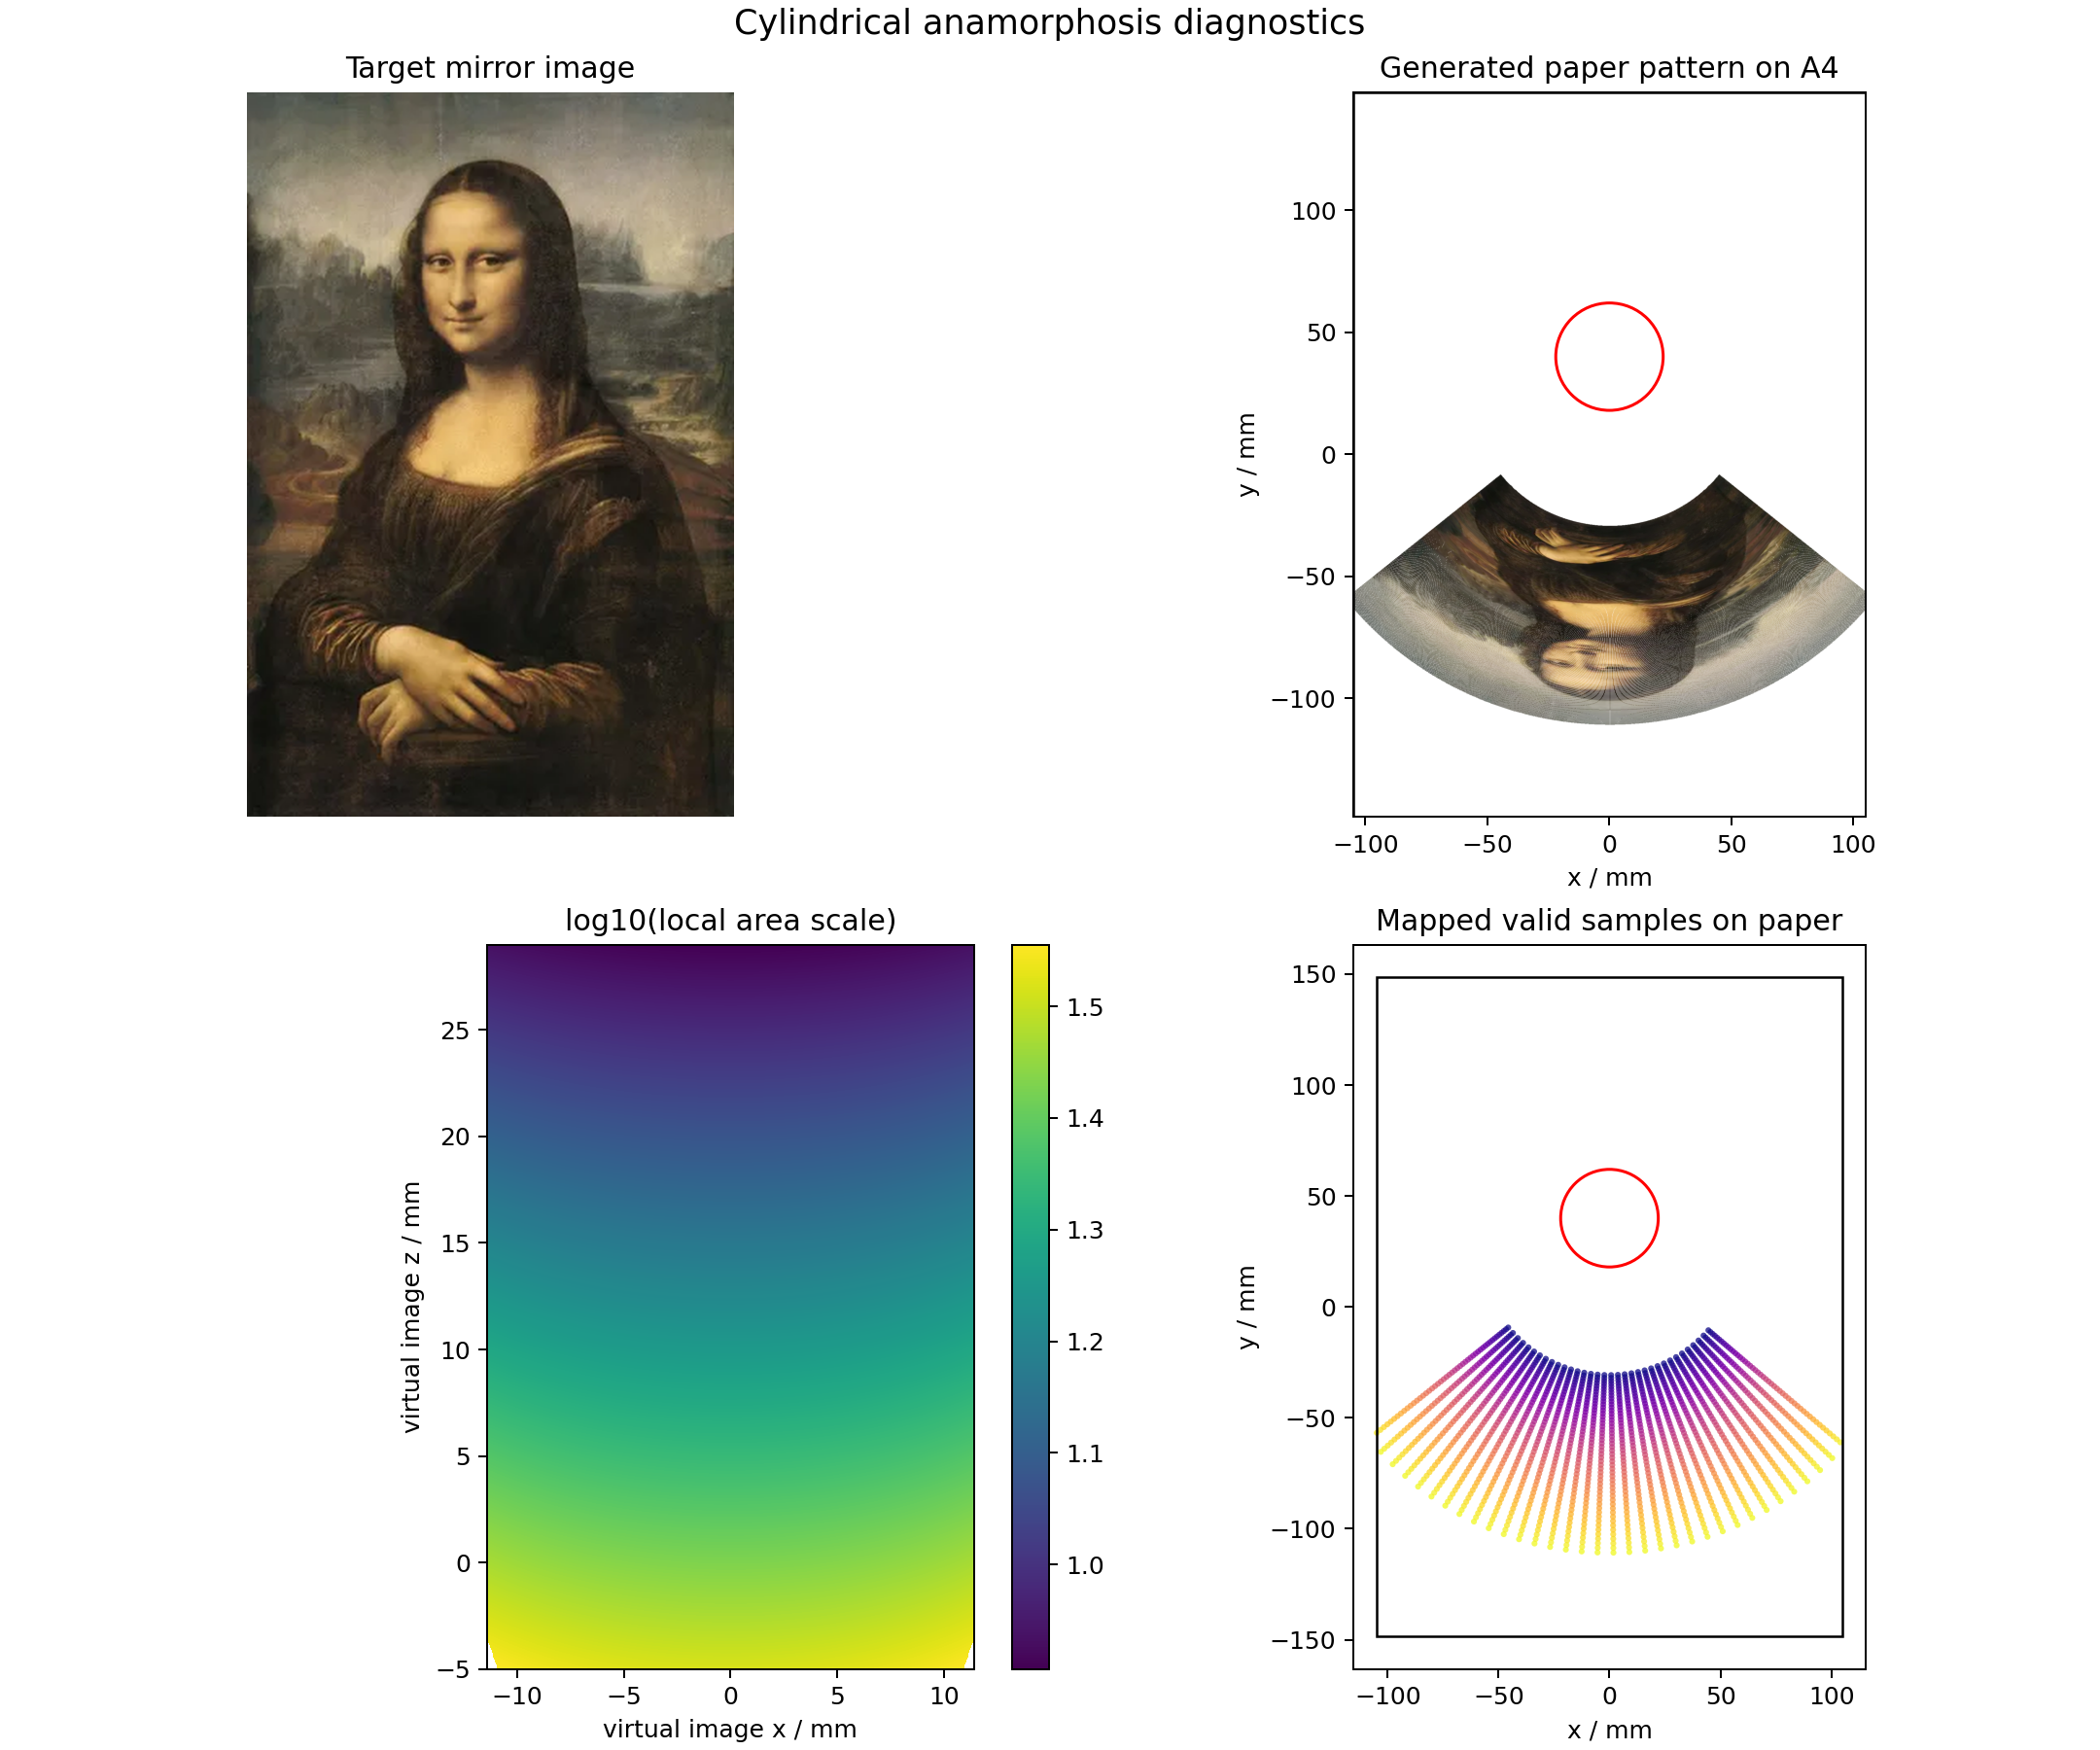
\includegraphics[width=\textwidth]{../outputs/cylindrical_anamorphosis/fig3_diagnostic.png}
\subcaption{图3 几何诊断}
\label{fig:fig3_diag}
\end{minipage}
\begin{minipage}[c]{0.49\textwidth}
\centering
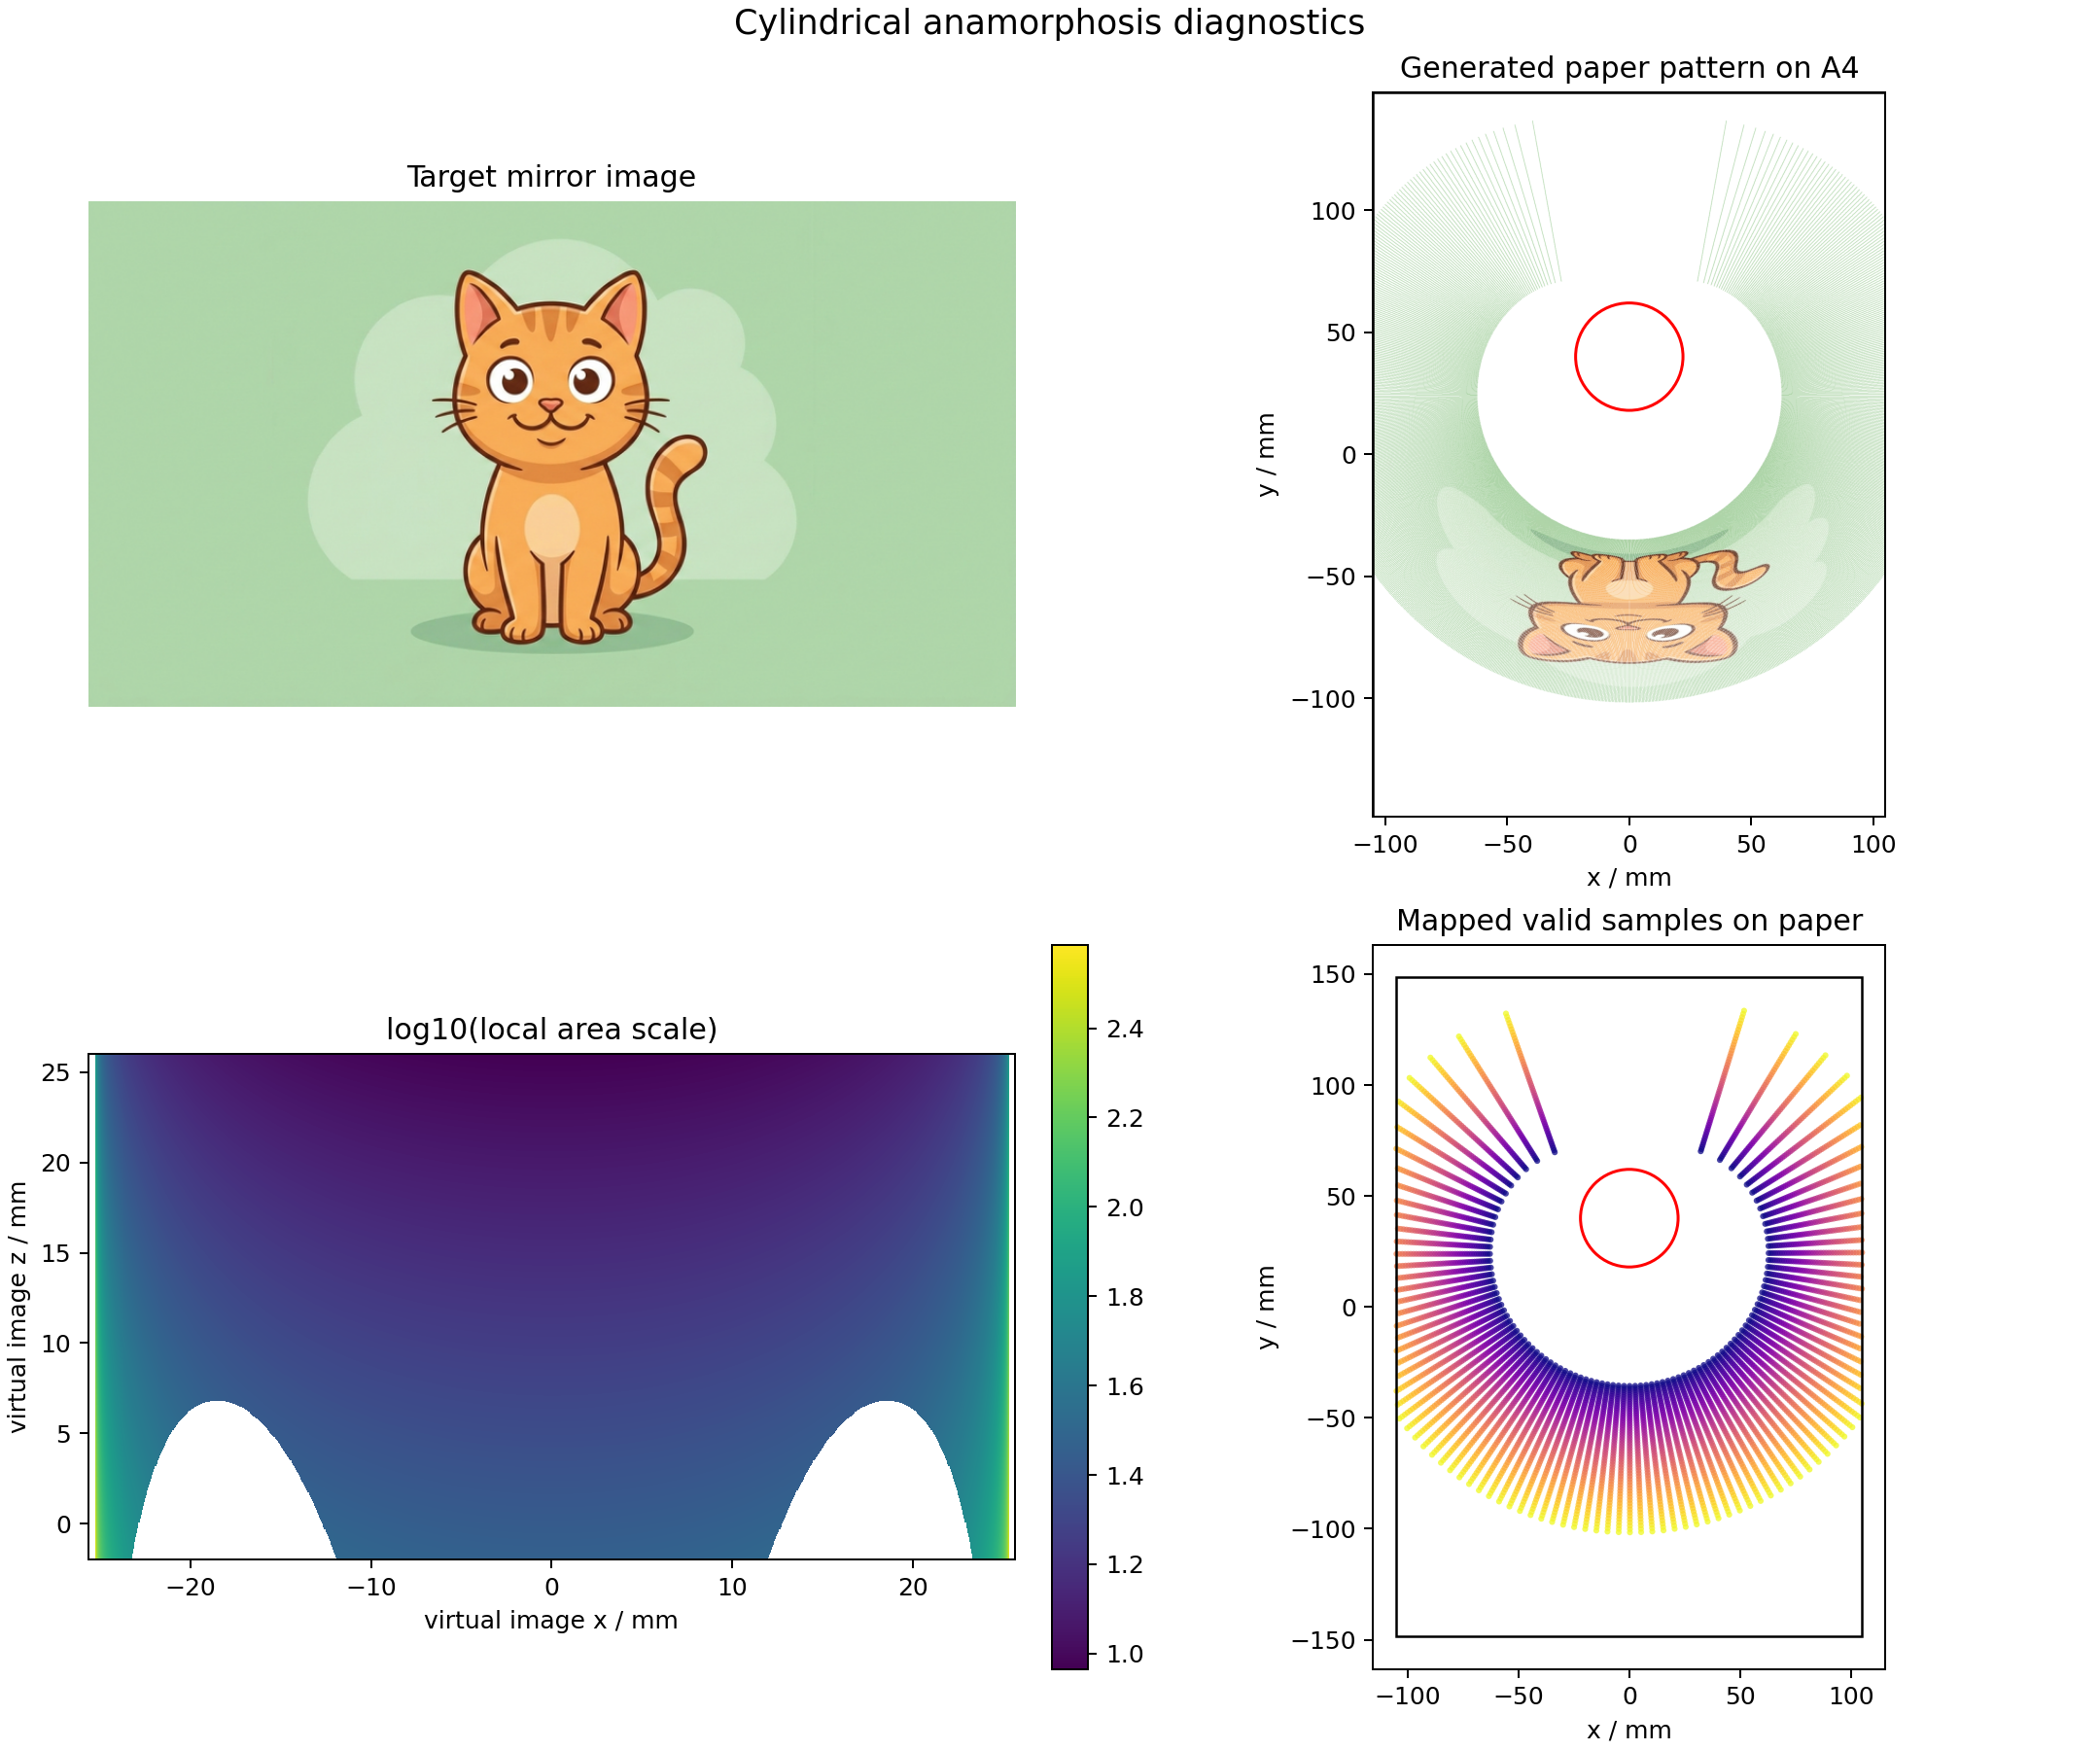
\includegraphics[width=\textwidth]{../outputs/cylindrical_anamorphosis/fig4_diagnostic.png}
\subcaption{图4 几何诊断}
\label{fig:fig4_diag}
\end{minipage}
\caption{几何诊断可视化。每幅诊断图包含四个子图：左上为目标镜面图像，右上为生成的 A4 纸面图案（红色圆圈为圆柱底座位置），左下为局部面积缩放因子 $\log_{10}$ 热力图，右下为有效采样点在纸面上的分布。}
\label{fig:diagnostics}
\end{figure}

\par 图 \ref{fig:diagnostics} 提供了逆反射映射的几何诊断信息。左下的面积缩放热力图显示，图3 的缩放因子分布在 1.0--1.5 之间，变化较为平缓；图4 的缩放因子分布范围更宽（1.0--2.4），反映了其横向构图在柱面反射中产生的更强拉伸。右下的有效采样点分布直观展示了纸面图案的覆盖范围：图3 呈扇形分布，图4 呈环形分布，均与纸面图案的实际形态一致。

\par 几何诊断结果与问题一中的参数优化结论相互印证：图3 由于纵向构图的特点，在柱面反射中产生的畸变较为均匀，缩放因子变化范围窄，有利于保持图像的视觉一致性；图4 由于横向构图导致的更强拉伸，缩放因子变化范围更宽，但仍在可接受范围内。这一发现也解释了为什么图3 的 A4 有效率（99.9\%）高于图4（89.3\%）——更均匀的畸变分布意味着更少的像素被映射到纸张边界之外。

\subsection{候选几何配置权衡分析}

\par 在确定推荐几何配置的过程中，本文对多组候选参数进行了系统性的横向比较。候选参数空间覆盖了圆柱中心位置、半径、观察点坐标、虚拟像平面位置等关键维度的合理取值范围。通过综合评分机制，将覆盖率、畸变水平和双图像通用性三项指标加权融合，筛选出最优的公共几何配置。

\par 候选方案的比较并不是简单地寻找某一个数值指标的最大值，而是要排除三类不适合制作的情形：其一，覆盖率较高但 Jacobian 条件数过大，说明图案虽然能落入纸面，却会出现强烈局部拉伸；其二，畸变较小但有效区域过窄，说明纸面利用不足，目标图像容易被裁切；其三，对图3 表现良好但对图4 明显失效，说明该参数缺乏公共适配性。只有同时避开这三类风险的候选方案，才适合作为最终推荐配置。

\par 因此，本节的候选配置比较主要服务于“为什么选择这一组参数”的解释，而非单纯展示搜索结果。若多个方案在总评分上接近，则优先选择覆盖率更稳定、两幅图像表现更均衡且参数更便于实际摆放的方案，这一原则也与竞赛题目强调的可复现制作要求一致。

\begin{figure}[H]
\centering
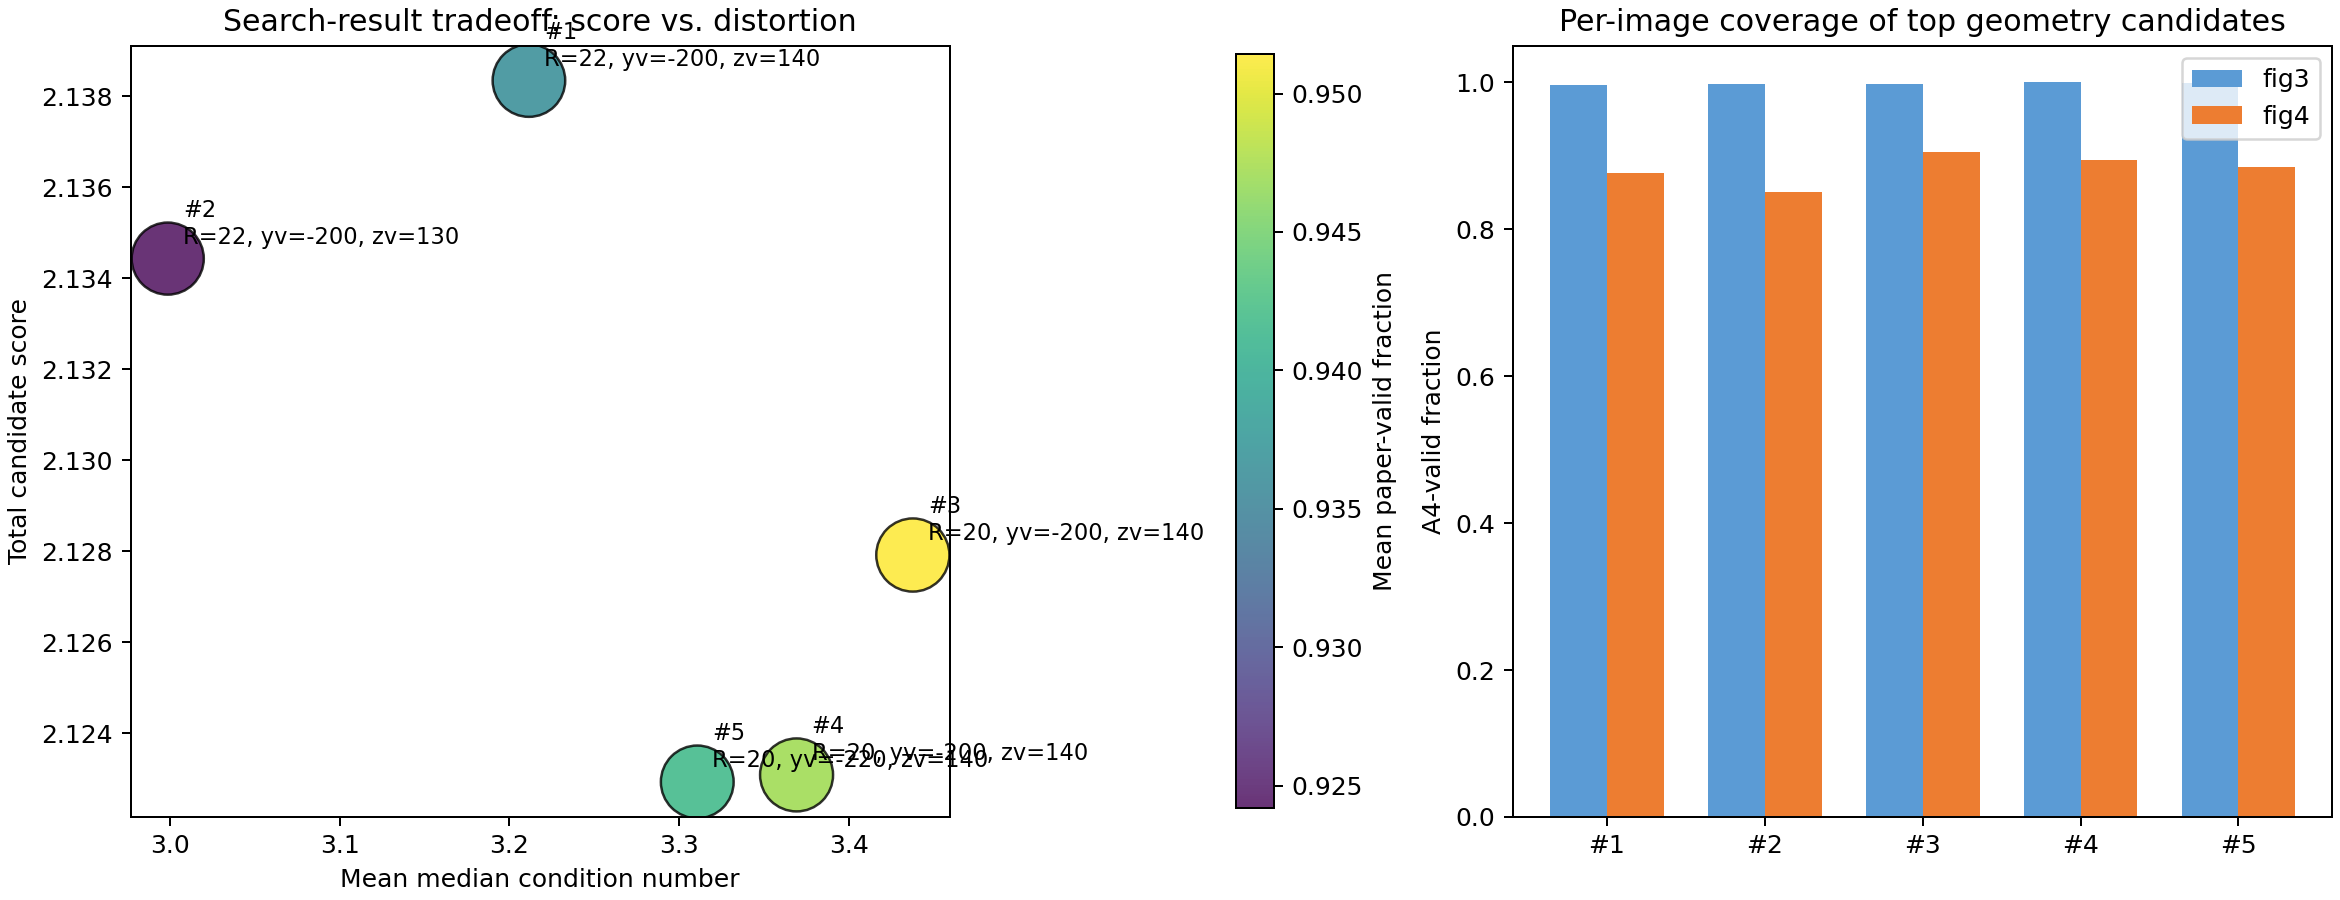
\includegraphics[width=\textwidth]{../outputs/cylindrical_anamorphosis/candidate_tradeoff_comparison.png}
\caption{候选几何配置的权衡分析}
\label{fig:tradeoff}
\end{figure}

\par 图 \ref{fig:tradeoff} 对候选配置的综合评分、畸变水平和覆盖率进行了横向比较。最终选取的公共几何参数并不是单项指标最优，而是在低畸变、高覆盖率和双图像通用性之间取得了较均衡的折中。

\par 从左侧散点图可以进一步看出，不同候选方案并未沿着“条件数越小、总评分越高”的单调规律分布，而是表现出明显的多目标竞争关系。例如，编号靠前的方案虽然在畸变控制上更有优势，但对应的有效覆盖率并不占优；相反，一些覆盖率更高的方案往往伴随更大的局部拉伸和更高的 Jacobian 条件数。也就是说，若只追求图像畸变最小，纸面可用区域会被压缩；若只追求纸张利用率最大，则又可能牺牲镜面成像的稳定性。

\par 右侧柱状图则反映了另一层更贴近赛题要求的信息：同一组几何参数对图3 和图4 的适配程度并不一致。图3 作为纵向构图，在前几组候选参数下都保持了接近满幅的覆盖率；图4 由于横向展开更明显，对参数变化更敏感，是决定公共参数优劣的关键约束项。因此，最终方案虽然不是“某一幅图像”的最佳方案，却是“同时兼顾两幅图像”的最稳妥方案。这样的选择更符合竞赛论文的评价标准，因为评审关注的通常不是单个指标峰值，而是整体方案的平衡性、可解释性与可复现性。

\par 从工程实现角度看，这一结果也说明本文采用的综合评分机制是合理的。它没有把覆盖率、畸变或双图像兼容性中的任意一项绝对化，而是强调在实际制作条件下寻找一个能够稳定工作的参数窗口。对于需要落地展示的反射变形装置而言，这种“稳中求优”的参数选择原则比单纯追求最优数值更有实际意义。

\subsection{单参数灵敏度分析}
\par 为了进一步说明最优参数并非偶然命中，而是处在一个具有可解释结构的局部稳定区间内，本文对圆柱中心位置、圆柱半径、观察点坐标、虚拟像平面位置以及虚拟像中心高度等关键参数进行了单因素扰动分析。分析时每次只改变一个参数，并保持其余参数不变，从而考察综合评分与最小覆盖率如何响应单参数变化。该方法能够直接揭示“哪一个参数更关键”“关键参数应向哪个方向调整”以及“当前最优值是否位于鲁棒区间内”等问题。

\par 与简单给出灵敏度排序相比，这种逐参数扫描更适合本题。原因在于圆柱镜面反射模型的几何含义非常直观：不同参数分别对应圆柱位置、镜柱大小、观察视角和虚拟像面布置，它们对成像的影响路径不同，且往往会以“提升一种指标、牺牲另一种指标”的方式出现。因此，只有把综合评分和覆盖率同时放到同一张图里，才能真正看出参数调整带来的收益与代价。

\par 灵敏度分析的具体实施方法如下：对每个关键参数，在推荐值附近取 11 个等间距采样点（扰动范围为推荐值的 $\pm 20\%$），对每个采样点重新运行完整的逆反射链计算，记录综合评分、最小覆盖率和 Jacobian 条件数分布。这种逐参数扫描虽然计算量较大，但能够清晰揭示每个参数的独立影响，避免多参数耦合带来的解释困难。

\begin{figure}[H]
\centering
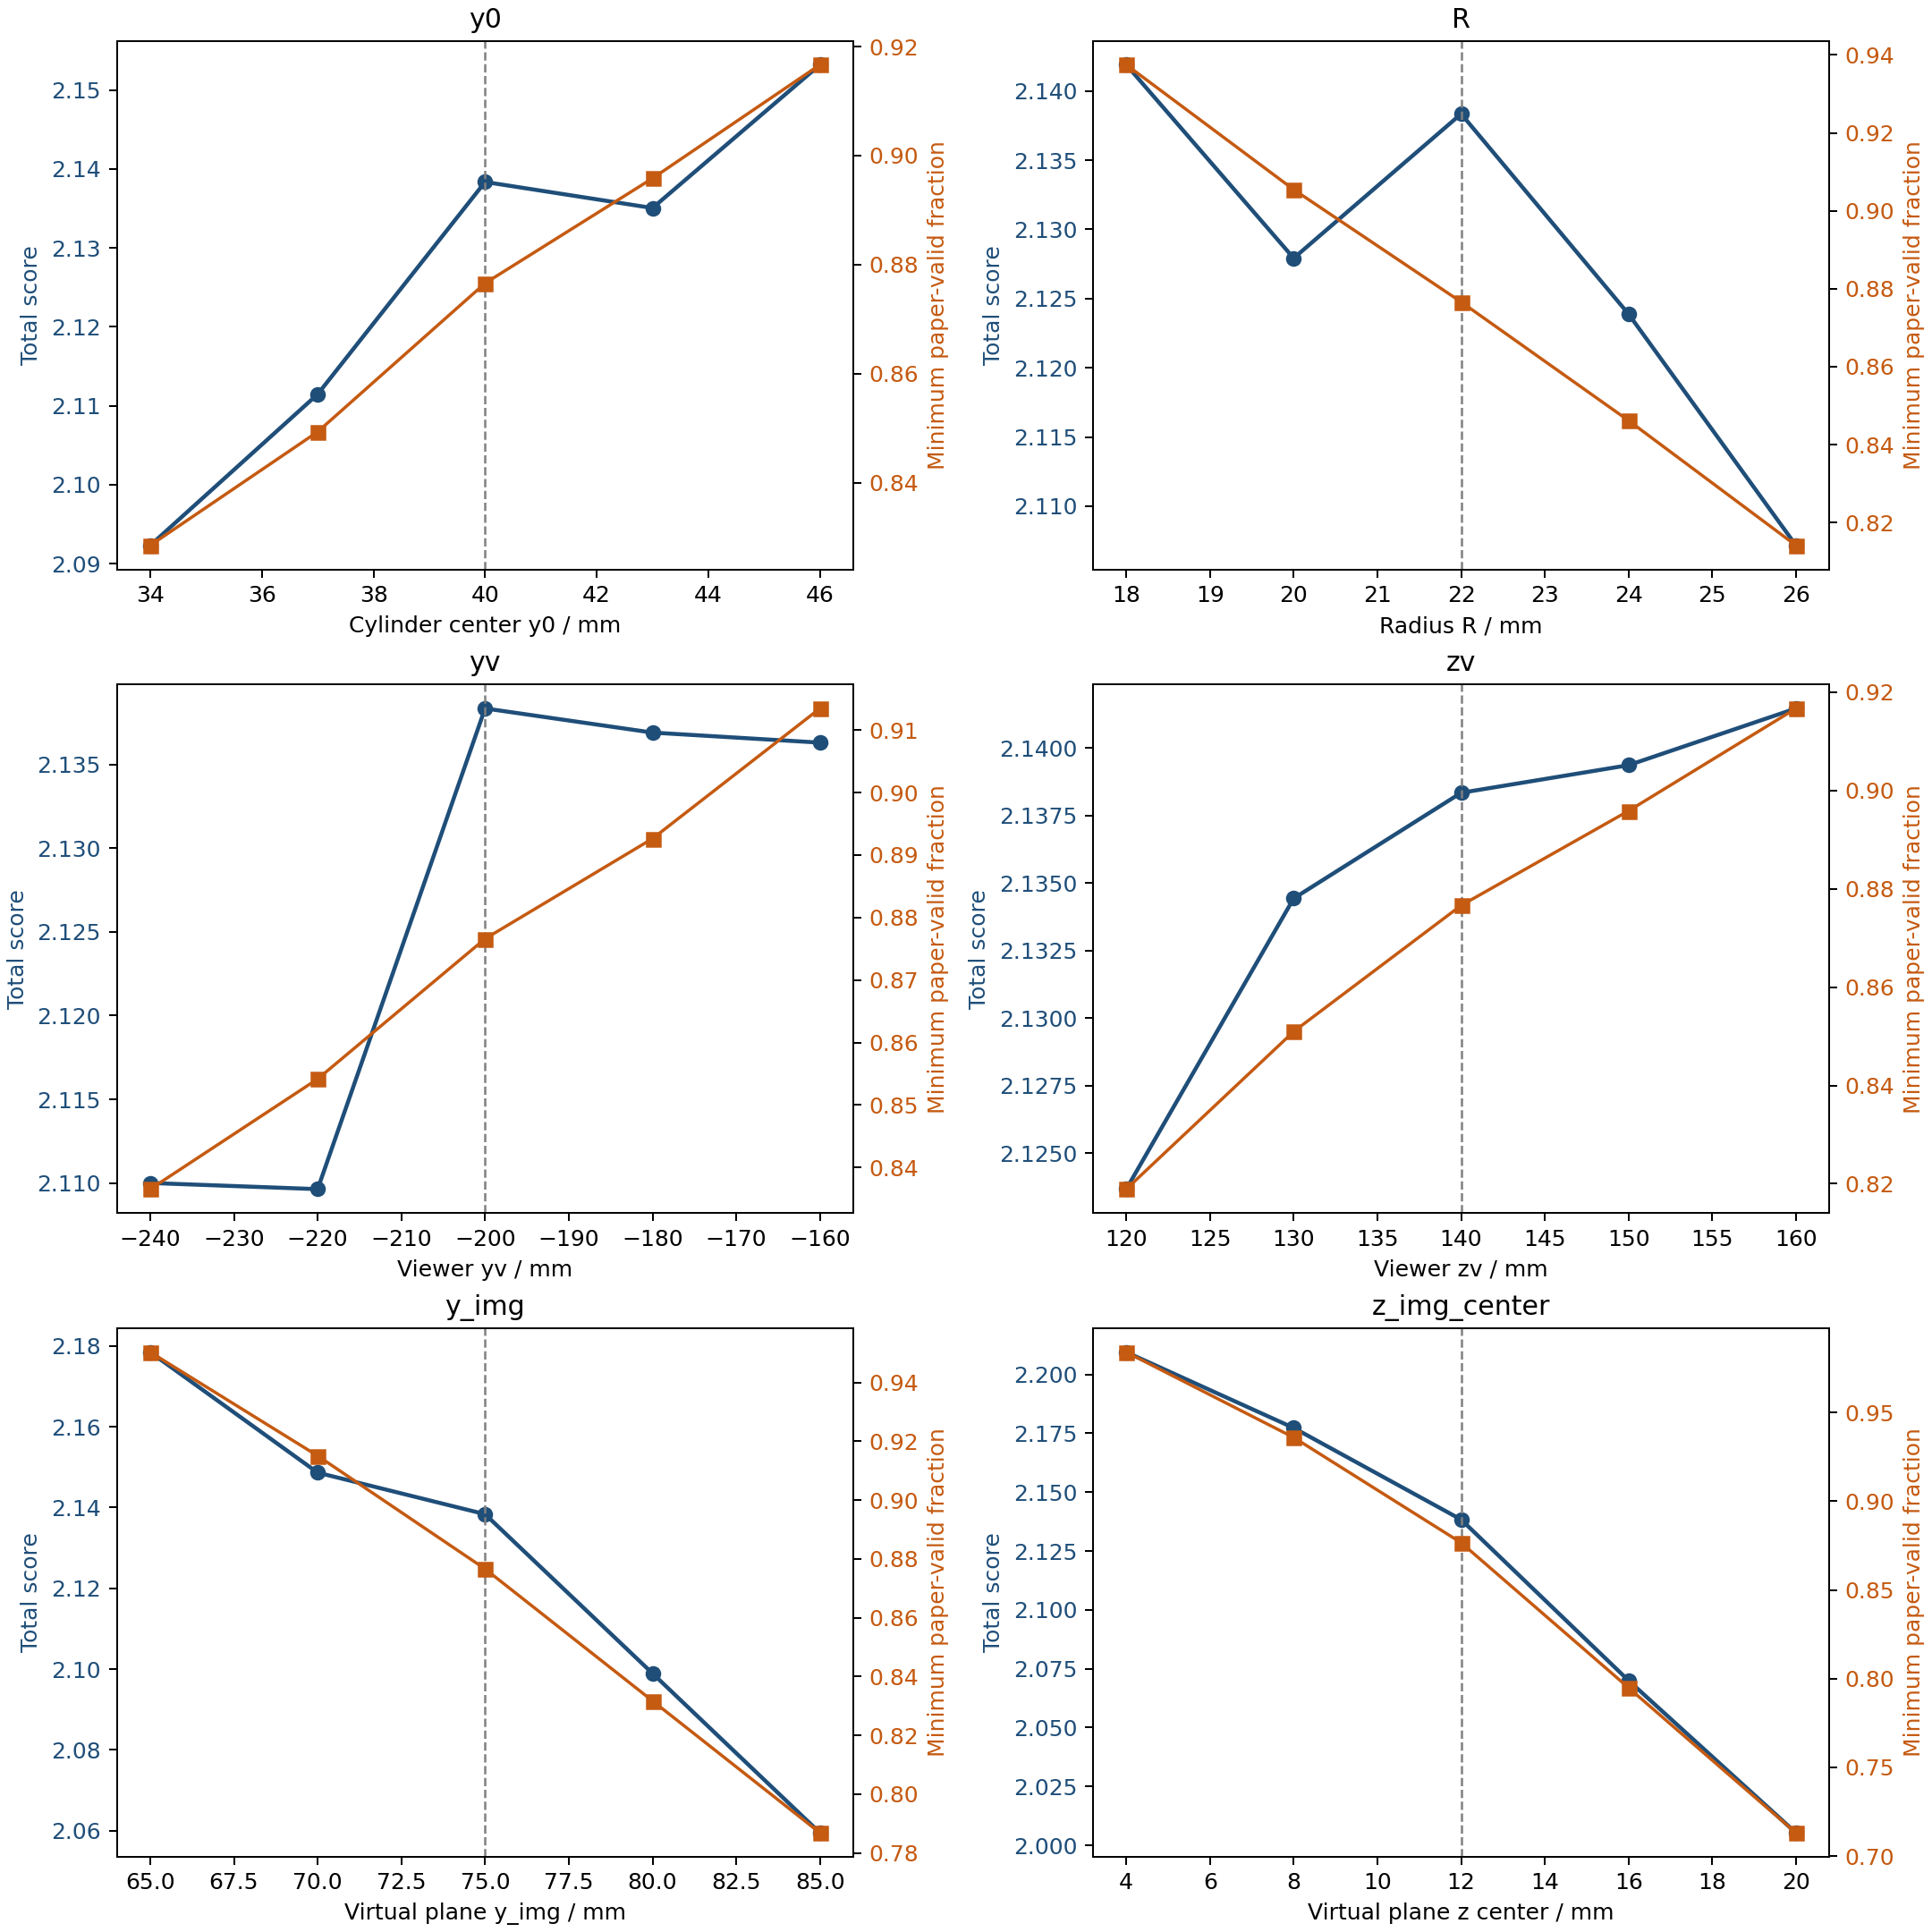
\includegraphics[width=\textwidth]{../outputs/cylindrical_anamorphosis/sensitivity_score_and_coverage.png}
\caption{综合评分与纸张覆盖率的灵敏度分析。横轴为各关键参数的扰动值，纵轴为综合评分（左）和最小覆盖率（右）。红色竖线标记推荐参数值。}
\label{fig:sensitivity_score}
\end{figure}

\par 图 \ref{fig:sensitivity_score} 展示了综合评分和最小覆盖率对各关键参数的响应曲线。从图中可以清晰看出，虚拟像平面位置 $y_{img}$ 和虚拟像中心高度 $z_{center}$ 的曲线斜率最大，说明这两个参数对模型表现的影响最为敏感。观察点高度 $z_v$ 和观察距离 $|y_v|$ 的曲线相对平缓，说明方案在实际搭建时具有一定的容错空间——即使观察者的身高或站立位置与推荐值有小幅偏差，也不会显著影响成像质量。

\begin{figure}[H]
\centering
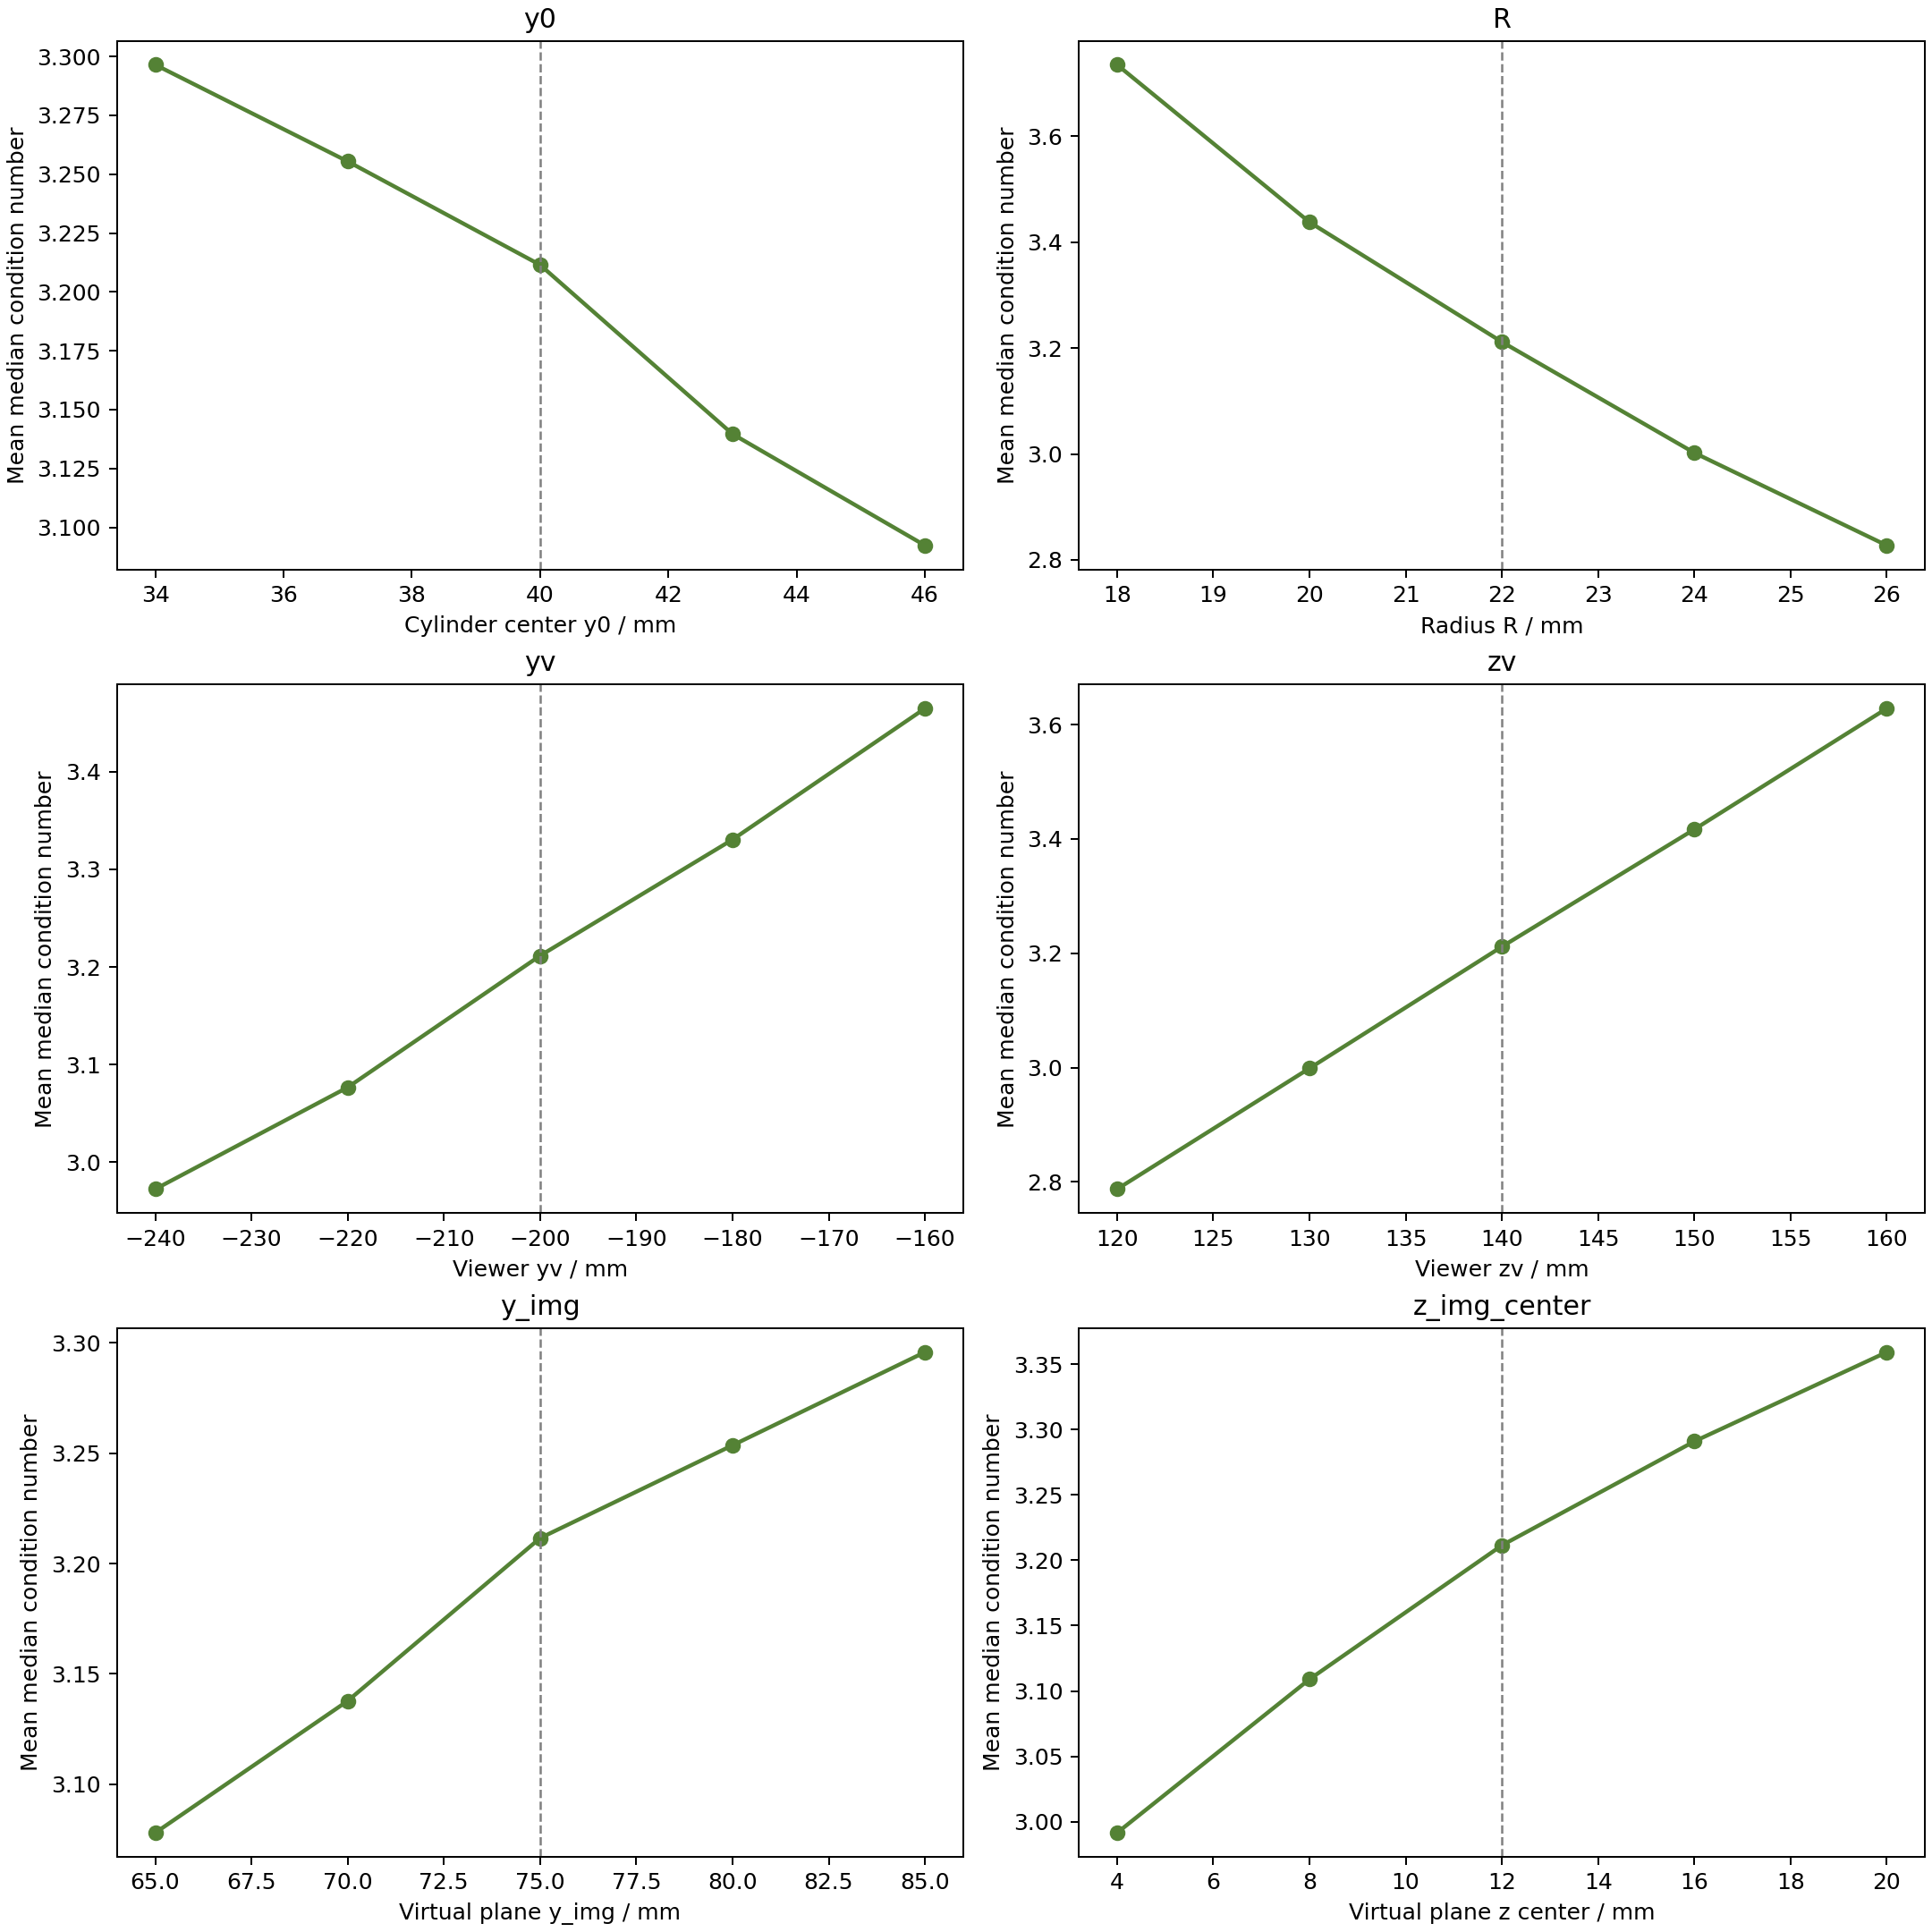
\includegraphics[width=\textwidth]{../outputs/cylindrical_anamorphosis/sensitivity_condition_numbers.png}
\caption{Jacobian 条件数分布的灵敏度分析。箱线图展示了各参数扰动下条件数的分布变化，红色竖线标记推荐参数值。}
\label{fig:sensitivity_cond}
\end{figure}

\par 图 \ref{fig:sensitivity_score} 和图 \ref{fig:sensitivity_cond} 表明，虚拟像平面位置 $y_{img}$ 和虚拟像中心高度 $z_{center}$ 对模型表现影响最明显。当前最优配置附近，适当减小 $y_{img}$ 通常有助于提升覆盖率并降低条件数；观察点高度和观察距离的影响相对平缓，说明方案在实际搭建时具有一定容错性。

\par 图 \ref{fig:sensitivity_cond} 的箱线图进一步揭示了条件数分布的变化规律。对于 $y_{img}$ 和 $z_{center}$ 这两个高灵敏度参数，当它们偏离推荐值时，不仅条件数的中位数上升，分布的离散程度也显著增大——这意味着局部畸变不仅整体变差，而且变得不均匀。相比之下，圆柱半径 $R$ 的条件数分布变化主要体现在中位数的平移，离散程度变化较小，说明半径调整对畸变的影响更为均匀可控。

\par 更细致地看，圆柱中心纵向位置 $y_0$ 与观察点纵向位置 $y_v$ 的变化主要影响纸面图案在 A4 区域内的整体分布位置。当这两个参数共同决定的投影区域向纸张中心靠拢时，最小覆盖率和综合评分通常同步上升；一旦图案整体偏向边缘，就会很快触发可用面积下降。相比之下，圆柱半径 $R$ 更多影响的是局部变形强度和纸面压缩程度。半径过小时，镜面曲率过大，会造成部分区域畸变集中；半径过大时，圆柱自身占据的纸面空间增加，可用于布置图案的区域反而被挤压。

\par 对虚拟像平面参数而言，$y_{img}$ 与 $z_{center}$ 的灵敏度最高，这与问题一中的几何分析是吻合的。$y_{img}$ 决定了目标像面与圆柱之间的距离，相当于控制了“镜面图像恢复的尺度基准”；$z_{center}$ 决定了有效成像区域更多落在圆柱的上部还是中下部，从而直接影响纸面图案在纵向上的展开方式。图中可以看到，当这两个参数偏离推荐值时，综合评分与最小覆盖率都会出现同步下滑，说明它们不仅影响图像质量，也影响方案是否还能完整落入 A4 纸面。

\par 另一方面，图 \ref{fig:sensitivity_cond} 给出的条件数分布也提供了重要补充：有些参数虽然对总评分影响看似有限，但会明显改变局部畸变的离散程度。换言之，平均指标相近并不代表图案视觉效果完全相同。若条件数分布变宽，就意味着某些局部区域会出现更明显的拉伸或压缩，从制作角度看，这类方案往往更依赖打印精度和观察位置的稳定性。因此，本文最终选择的参数不仅在平均意义上较优，也在分布意义上更稳健。

\subsection{灵敏度分析结论}
\par 综合来看，本文模型对关键几何参数的响应是清晰可解释的：虚拟像平面过远会增加畸变不均匀性，圆柱半径过大则会压缩有效纸面区域，而观察点高度在合理范围内波动时对结果影响较小。这说明模型既具有可调性，也具有一定工程鲁棒性。

\section{模型评价与推广}

\subsection{模型优点}
\begin{compactitem}
\item 以几何光学为基础，模型推导路径清晰，物理含义明确；单视点核心模型配合双目稳定性扩展检验，兼顾理论严谨性与实际鲁棒性。
\item 从问题一到问题三形成了由"可生成"到"可兼容"的递进分析链条，逻辑完整；问题三明确区分平面纸张自由度约束与自由曲面显示的本质差异，建模定位清晰。
\item 将 A4 约束、圆柱间隙、Jacobian 畸变和双目一致性纳入统一分析框架，结果具有制作指导意义。
\item 配套给出了几何示意图、流程图、验证图、灵敏度图、双目观察几何图和空间场景合成可视化，支撑材料较为完整。
\end{compactitem}

\subsection{模型局限性}
\begin{compactitem}
\item 采用理想镜面假设，尚未考虑真实镜面加工误差和反射损耗。
\item 核心模型基于单一观察点，双目视觉一致性仅作为稳定性扩展检验，而非临床视觉科学意义上的严格约束。
\item 双指定图案部分主要给出近似兼容性判据和理论思路，尚未做大规模实例穷举验证；自由曲面显示领域的研究仅作为类比支撑，而非直接求解方法。
\item 空间可视化均为合成渲染结果，非真实物理实验场景。
\end{compactitem}

\subsection{模型推广}
\begin{compactitem}
\item 将圆柱面替换为圆锥面、球面或椭圆柱面后，逆反射链思想仍可继续使用。
\item 可用于分析防伪标签、舞台装置、互动展陈等需要"平面编码-镜面解码"的应用场景。
\item 单视点核心模型配合双目稳定性检验的框架可推广至其他几何光学问题，为"核心模型+扩展验证"的两阶段分析提供参考范式。
\item 平面纸张自由度约束下的近似兼容性分析方法，可为其他受限媒介的变形设计问题提供借鉴思路。
\end{compactitem}

\begin{thebibliography}{99}
\bibitem{ref1} 华中杯数学建模竞赛组委会. 反射的艺术[B]. 2025.
\bibitem{ref2} 司守奎. 数学建模算法与程序[M]. 北京: 国防工业出版社, 2015.
\bibitem{ref3} 姜启源, 谢金星, 叶俊. 数学模型[M]. 北京: 高等教育出版社, 2011.
\bibitem{ref4} Hartley R, Zisserman A. Multiple View Geometry in Computer Vision[M]. Cambridge: Cambridge University Press, 2004.
\bibitem{ref5} Szeliski R. Computer Vision: Algorithms and Applications[M]. Springer, 2022.
\bibitem{ref6} Wu J, et al. Computational Mirror Cup and Saucer Art[J]. ACM Transactions on Graphics, 2022, 41(4): 1-15.
\end{thebibliography}

\newpage
\begin{appendices}

\section{核心算法伪代码}

\begin{lstlisting}[language=Python]
def inverse_reflection_chain(P_img, V, cylinder, paper_z=0):
    """
    从虚拟像点反推纸面点的逆反射链
    """
    d_view = P_img - V
    t = intersect_line_cylinder(V, d_view, cylinder)
    P_cyl = V + t * d_view

    n = compute_cylinder_normal(P_cyl, cylinder)
    d_out = normalize(P_img - P_cyl)
    d_in = d_out - 2 * dot(d_out, n) * n

    s = -P_cyl[2] / d_in[2]
    P_paper = P_cyl + s * d_in
    return P_paper


def compute_jacobian(P_img, theta, eps=1e-6):
    """
    用数值微分近似 Jacobian
    """
    J = zeros((2, 2))
    P0 = inverse_reflection_chain(P_img, theta.viewer, theta.cylinder)
    for i in range(2):
        P_shift = P_img.copy()
        P_shift[i] += eps
        P_shift_paper = inverse_reflection_chain(P_shift, theta.viewer, theta.cylinder)
        J[:, i] = (P_shift_paper[:2] - P0[:2]) / eps
    return J
\end{lstlisting}

\section{Python 实现代码}

\subsection{变形图案生成主程序}
\par 该程序包含完整的几何参数搜索模块、逆反射链实现、图案栅格化以及诊断可视化功能。程序入口为 \texttt{generate\_patterns.py}，核心逻辑围绕"虚拟像点→圆柱交点→纸面点"的逆映射展开，支持多组几何候选配置的性能对比与自动筛选。

\subsection{分析与可视化程序}
\par 该程序负责生成全文所有分析图表，包括：目标图像与虚拟像平面配置图、几何参数搜索散点图与柱状图、回采重建对比图、灵敏度分析曲线图、Q2 自由设计画廊、Q2 指定镜面画廊、Q3 兼容性相图与热力图以及代表性案例展示。程序入口为 \texttt{generate\_analysis\_assets.py}，所有输出图像均保存于 \texttt{outputs/cylindrical\_anamorphosis/} 目录。

\section{支撑材料清单}
\par 本文研究过程中的主要支撑材料如下。

\par \textbf{输入图像：}位于 \texttt{附件} 目录中的图3 和图4 原始图片。

\par \textbf{生成结果：}位于 \texttt{outputs/cylindrical\_anamorphosis/} 目录中的纸面图案、诊断图、占用图、几何示意图、流程图、回采验证图以及灵敏度分析图。

\par \textbf{结构化报告：}包括 \texttt{parameter\_report.json} 与 \texttt{validation\_metrics.json}，分别记录几何搜索结果和验证指标。

\par \textbf{源码文件：}
\begin{compactitem}
\item \texttt{anamorphosis/generate\_patterns.py}
\item \texttt{anamorphosis/generate\_analysis\_assets.py}
\end{compactitem}

\end{appendices}

\end{document}
